\documentclass[10pt]{memoir}
\setstocksize{220mm}{155mm} 	        
\settrimmedsize{220mm}{155mm}{*}	
\settypeblocksize{170mm}{116mm}{*}	
\setlrmargins{18mm}{*}{*}
\setulmargins{*}{*}{1.2}
%\setlength{\headheight}{5pt}%
\checkandfixthelayout[lines]
\linespread{1.16}
\flushbottom

%%% Hyphenation settings
\usepackage[htt]{hyphenat}
\hyphenation{he-lio-trope opos-sum}
\tracingparagraphs=1
%Hyphenation in Devanāgarī of the edition still missing? Probably this needs to be modified in babel-iast package? 

%%% babel
\usepackage[english]{babel}
\usepackage{babel-iast/babel-iast}

\babelfont[iast]{rm}[Renderer=Harfbuzz, Scale=1.3]{AdishilaSan}%AdishilaSan}
\babelfont[english]{rm}{Adobe Text Pro}

%%% more functionality
\PassOptionsToPackage{hyphens}{url}
\usepackage{hyperref}
\usepackage{pdflscape}
\usepackage{cleveref}
\usepackage{url}
\usepackage{cleveref}
\usepackage{microtype}
\usepackage{lineno}

%\usepackage{bigfoot}
%%% more functions
\usepackage[dvipsnames]{xcolor}
%\usepackage[para,perpage]{footmisc}

%%%für den Counter von Kapiteln und Sätzen! 
\newcommand{\uproman}[1]{\uppercase\expandafter{\romannumeral#1}}
\newcommand{\lowroman}[1]{\romannumeral#1\relax}

\makeindex
\newfontfamily\sanskritfont[Script=Devanagari,Mapping=RomDev,Scale=1.1]{Sanskrit2003}
\usepackage{pifont,fourier-orns,lettrine,psvectorian,paralist,enumitem,pdfpages,wrapfig,tabulary,lettrine,longtable}
\setlist[enumerate]{itemsep=0mm}
\usepackage[autostyle]{csquotes}
\usepackage[defaultlines=2,all]{nowidow}
\usepackage{ellipsis,adforn,booktabs,longtable,url,tikz}
\lineskiplimit=-3pt          

\makechapterstyle{IeT}{%
  \chapterstyle{default}
  \renewcommand*{\printchapternonum}{\centering}
  \renewcommand*{\clearforchapter}{\cleartorecto} 
  \aliaspagestyle{chapter}{empty}}
\chapterstyle{IeT}
\setsecnumdepth{none}  \openright  \nouppercaseheads
\settocdepth{subsubsection}

%%%% test better pagebreaks
%\def\fussy{%
%  \emergencystretch\z@
%  \tolerance 200%
%  \hfuzz .1\p@
%  \vfuzz\hfuzz}

%\interfootnotelinepenalty=10000\relax

%\usepackage[maxfloats=256]{morefloats}

%\maxdeadcycles=500

%raggedbottomsectiontrue
%%\checkandfixthelayout


%%%%%%%  biblatex
%\newcommand{\noun}[1]{\textsc{#1}}    %  philosophy-verbose
\usepackage[backend=biber, sorting=nyt, style=verbose]{biblatex} %%%%ORIGINAL TiE
\renewcommand*{\mkbibnamefamily}[1]{\textsc{#1}}


\DeclareFieldFormat{url}{%
  \mkbibacro{URL}\addcolon\space
  \href{#1}{\nolinkurl{\thefield{urlraw}}}}

\DeclareFieldFormat{citeurl}{%
  \href{#1}{\nolinkurl{\thefield{urlraw}}}} 


\DeclareFieldFormat{postnote}{#1}
\renewcommand{\postnotedelim}{, }
\addbibresource{bindu.bib}

%%% ekdosis
\usepackage[teiexport=tidy,parnotes=true]{ekdosis}% =tidy cleans up HTML and XML documents by fixing markup errors and upgrading legacy code to modern standards. parnotes=footnotes below or above critical apparatus

\SetLineation{lineation=page, modulo} %lineation=page sets thenumbering to start afresh at the top of each page. =modulo makes every fifth line numbered. {lineation=page} makes every line numbered! 

\renewcommand{\linenumberfont}{\selectlanguage{english}\footnotesize} %sets language of lines to English

\SetTEIxmlExport{autopar=false} %autopar=falseinstructs ekdosis to ignore blank lines in the.tex sourcefile as markers for paragraph boundaries. As a result, each paragraph of the edition must be found within an environment associated with the xml <p> element

\SetHooks{
  lemmastyle=\bfseries,
  %refnumstyle=\selectlanguage{english}\bfseries,
  refnumstyle=\selectlanguage{english}\color{blue}\bfseries,
  appheight=0.8\textheight,
}

\newif\ifinapparatus
\DeclareApparatus{source}[
%bhook=\inapparatustrue,
lang=english,
notelang=english,
% bhook=\selectlanguage{english},
bhook=\selectlanguage{english}\textbf{Sources:},%
%maxentries=4, 
%ehook=.]
%sep={] },
%nosep,
]

\newif\ifinapparatus
\DeclareApparatus{testium}[
%bhook=\inapparatustrue,
lang=english,
notelang=english,
% bhook=\selectlanguage{english},
bhook=\selectlanguage{english}\textbf{Testimonia:},
%maxentries=4, 
%ehook=.]
%nosep, 
]

% Declare \ifinapparatus and set \inapparatustrue at the beginning of
% the apparatus criticus block. Also set the language.  
\newif\ifinapparatus
  \DeclareApparatus{default}[
  %bhook=\inapparatustrue, 
  lang=english,
  %maxentries=33,
  %bhook=\selectlanguage{english},
  sep = {] },
  delim=\hskip 0.75em,
  rule=\rule{0.7in}{0.4pt},
]

\newif\ifinapparatus
\DeclareApparatus{philcomm}[
%bhook=\inapparatustrue,
lang=english,
notelang=english,
bhook=\selectlanguage{english}\textbf{Philological Commentary:},
%bhook=\selectlanguage{english},
sep={: },
]

\ekdsetup{
showpagebreaks,
spbmk = \textcolor{blue}{spb},
hpbmk = \textcolor{red}{hpb}
}

%\usepackage{fnpos}
%\makeFNmid
%\makeFNbottom
\usepackage[bottom]{footmisc}
%%%%%%%%%%%%%%%%%%%%%%%%%%%
\makeatletter
\def\blfootnote{\gdef\@thefnmark{}\@footnotetext}
\makeatother
%%%%%%%%%%%%%%%%%%%%%%%%%


% Macros and Definitions for the Print of Sigla
\def\acpc#1#2#3{{#1}\rlap{\textrm{\textsuperscript{#3}}}\textsubscript{\textrm{#2}}\space}
\def\sigl#1#2{{{#1}}\textsubscript{\textrm{#2}}}
\def\None{{\sigl{N}{1}}} \def\Noneac{\acpc{N}{1}{ac}\,} \def\Nonepc{\acpc{N}{1}{pc}\,}
\def\Ntwo{{\sigl{N}{2}}} \def\Noneac{\acpc{N}{2}{ac}\,} \def\Nonepc{\acpc{N}{2}{pc}\,}
\def\Done{{\sigl{D}{1}}} \def\Doneac{\acpc{D}{1}{ac}\,} \def\Donepc{\acpc{D}{1}{pc}\,}
\def\Dtwo{{\sigl{D}{2}}} \def\Dtwoac{\acpc{D}{2}{ac}\,} \def\Dtwopc{\acpc{D}{2}{pc}\,}
\def\Uone{{\sigl{U}{1}}} \def\Uoneac{\acpc{U}{1}{ac}\,} \def\Uonepc{\acpc{U}{1}{pc}\,}                 
\def\Utwo{{\sigl{U}{2}}} \def\Utwoac{\acpc{U}{2}{ac}\,} \def\Utwopc{\acpc{U}{2}{pc}\,}

%%%%%%%%%%%%%% Tattvabinduyoga - List of Witnesses   %%%%%%%%%%%%%%%%%%%
\DeclareWitness{ceteri}{\selectlanguage{english}cett.}{ceteri}[]   
\DeclareWitness{E}{\selectlanguage{english}E}{Printed Edition}[]    
\DeclareWitness{P}{\selectlanguage{english}P}{Pune BORI 664}[]  
\DeclareWitness{B}{\selectlanguage{english}B}{Bodleian 485}[]       
\DeclareWitness{N1}{\selectlanguage{english}N\textsubscript{1}}{NGMPP 38/31}[]
\DeclareWitness{N2}{\selectlanguage{english}N\textsubscript{2}}{NGMPP B 38/35}[]
\DeclareWitness{L}{\selectlanguage{english}L}{LALCHAND 5876}[]  
\DeclareWitness{D}{\selectlanguage{english}D}{IGNCA 30019}[] 
%\DeclareWitness{D2}{\selectlanguage{english}D\textsubscript{2}}{IGNCA 30020}[]  
\DeclareWitness{U1}{\selectlanguage{english}U\textsubscript{1}}{SORI 1574}[] 
\DeclareWitness{U2}{\selectlanguage{english}U\textsubscript{2}}{SORI 6082}[]
%%%%%%%%%%%%%% Tattvabinduyoga - Groups of Witnesses   %%%%%%%%%%%%%%%%%%%
\DeclareWitness{X}{\selectlanguage{english}\alpha}{Alpha Group: D,N1,N2,U1}[]
\DeclareWitness{Y}{\selectlanguage{english}\beta}{Beta Group: B,E,L,P,U2}[]
%%%%%%%%%%%%% Testimonia
\DeclareWitness{Ysv}{\selectlanguage{english}Ysv}{Yogasvarodaya}[] %%%add infos!  

%%%%%%%%%%%%%%%%%%%%%%%%%%%%%%%%%%%%%%%%%%%
% Macro for Editing Abbrevs.
\def\om{\textrm{\footnotesize \textit{om.}\ }} %prints om. for omitted in apparatus
\def\korr{\textrm{\footnotesize \textit{em.}\ }} %prints em. for emended in apparatus
\def\conj{\textrm{\footnotesize \textit{conj.}\ }} %prints conj. for conjectured in apparatus

% \supplied{text} EDITORIAL ADDITION -> Within \lem oder \rdg
% \surplus{text} EDITORIAL DELETION -> Within \lem oder \rdg
% \sic{text} CRUX
% \gap{text} LACUNAE -> [reason=??, unit=??, quantity=??, extent=??]


%%%%%%%%%%%%%%%%%%%%%%%%%%%%%%%%%%%%%%%%%%% All macros of this list can be used in 
% Macro for Editing Abbrevs.
\def\eyeskip{\textrm{{ab.\,oc. }}}
\def\aberratio{\textrm{{ab.\,oc. }}}
\def\ad{\textrm{{ad}}}
\def\add{\textrm{{add.\ }}}
\def\ann{\textrm{{ann.\ }}}
\def\ante{\textrm{{ante }}} 
\def\post{\textrm{{post }}}
%\def\ceteri{cett.\,}                   
\def\codd{\textrm{{codd.\ }}}

\def\coni{\textrm{{coni.\ }}}
\def\contin{\textrm{{contin.\ }}}
\def\corr{\textrm{{corr.\ }}}
\def\del{\textrm{{del.\ }}}
\def\dub{\textrm{{ dub.\ }}}

\def\expl{\textrm{{explic.\ }}} 
\def\explica t{\textrm{{explic.\ }}}
\def\fol{\textrm{{fol.\ }}}
\def\foll{\textrm{{foll.\ }}}
\def\gloss{\textrm{{glossa ad }}}
\def\ins{\textrm{{ins.\ }}}      
\def\inseruit{\textrm{{ins.\ }}} 
\def\im{{\kern-.7pt\lower-1ex\hbox{\textrm{\tiny{\emph{i.m.}}}\kern0pt}}} %\textrm{\scriptsize{i.m.\ }}}      
\def\inmargine{{\kern-.7pt\lower-.7ex\hbox{\textrm{\tiny{\emph{i.m.}}}\kern0pt}}}%\textrm{\scriptsize{i.m.\ }}}      
\def\intextu{{\kern-.7pt\lower-.95ex\hbox{\textrm{\tiny{\emph{i.t.}}}\kern0pt}}}%\textrm{\scriptsize{i.t.\ }}}           
\def\indist{\textrm{{indis.\ }}}  
\def\indis{\textrm{{indis.\ }}}
\def\iteravit{\textrm{{iter.\ }}} 
\def\iter{\textrm{{iter.\ }}}
\def\lectio{\textrm{{lect.\ }}}   
\def\lec{\textrm{{lect.\ }}}
\def\leginequit{\textrm{{l.n. }}} 
\def\legn{\textrm{{l.n. }}}
\def\illeg{\textrm{{l.n. }}}

\def\primman{\textrm{{pr.m.}}}
\def\prob{\textrm{{prob.}}}
\def\rep{\textrm{{repetitio }}}
\def\secundamanu{\textrm{\scriptsize{s.m.}}}            \def\secm{{\kern-.6pt\lower-.91ex\hbox{\textrm{\tiny{\emph{s.m.}}}\kern0pt}}}%   \textrm{\scriptsize{s.m.}}}
\def\sequentia{\textrm{{seq.\,inv.\ }}}  
\def\seqinv{\textrm{{seq.\,inv.\ }}}
\def\order{\textrm{{seq.\,inv.\ }}}
\def\supralineam{{\kern-.7pt\lower-.91ex\hbox{\textrm{\tiny{\emph{s.l.}}}\kern0pt}}} %\textrm{\scriptsize{s.l.}}}
\def\interlineam{{\kern-.7pt\lower-.91ex\hbox{\textrm{\tiny{\emph{s.l.}}}\kern0pt}}}   %\textrm{\scriptsize{s.l.}}}
\def\vl{\textrm{v.l.}}   \def\varlec{\textrm{v.l.}} \def\varialectio{\textrm{v.l.}}
\def\vide{\textrm{{cf.\ }}}
\def\cf{\textrm{{cf.\ }}} 
\def\videtur{\textrm{{vid.\,ut}}}
\def\crux{\textup{[\ldots]} }
\def\cruxx{\textup{[\ldots]}}
\def\unm{\textit{unm.}}
%%%%%%%%%%%%%%%%%%%%%%%%%%%%%%%%%%%%

% List of Scholars
\DeclareScholar{ego}{ego}[
forename=Nils Jacob,
surname=Liersch]

% Persons:14\DeclareScholar{ego}{ego}[15forename=Robert,16surname=Alessi]17% Useful shorthands:18\DeclareShorthand{codd}{codd.}{V,I,R,H}19\DeclareShorthand{edd}{edd.}{Lit,Erm,Sm}20\DeclareShorthand{egoscr}{\emph{scripsi}}{ego}

%Useful shorthands:
%\DeclareShorthand{codd}{codd.}{V,I,R,H}
%\DeclareShorthand{edd}{edd.}{Lit,Erm,Sm}
\DeclareShorthand{egoscr}{em.}{ego}
\DeclareShorthand{egoscrconj}{conj.}{ego}
\DeclareShorthand{egomute}{\unskip}{ego}

\usepackage{xparse}

\NewDocumentEnvironment{tlg}{O{}O{}}{\setlength{\leftskip}{0pt}\vspace{-1ex}\begin{quotation}}{\hfill #1\ \vspace{-1ex}\end{quotation}\vspace{-1ex}} %verse environment
%\NewDocumentEnvironment{tlg}{O{}O{}}{\begin{verse}}{॥#1\hskip-4pt ॥\\ \end{verse}}
\NewDocumentCommand{\tl}{m}{{\selectlanguage{iast} #1}}

\NewDocumentCommand{\extra}{m}{{\textcolor{gray}{#1}}} %command for additions to U2
\NewDocumentCommand{\crazy}{m}{{\textcolor{red}{#1}}} %totally corrupted passage
\NewDocumentCommand{\coro}{m}{{\textcolor{violet}{#1}}} %colour for sentence counter! 

\NewDocumentEnvironment{prose}{O{}}{\begin{otherlanguage}{iast}}{\end{otherlanguage}}
% \NewDocumentEnvironment{padd}{O{}}{\begin{otherlanguage}{iast}}{\end{otherlanguage}}
\NewDocumentEnvironment{tlate}{O{}}
%\NewDocumentEnvironment{tadd}{O{}}

%Define two commands: \skp ("sanskrit plus"), to be ignored by TeX in
%the edition text, but processed in the TEI output. Conversely, \skm
%("sanskrit minus") is to be processed in the edition text, but
%ignored if found in the apparatus criticus and in the TEI output:

\NewDocumentCommand{\skp}{m}{}
\TeXtoTEIPat{\skp {#1}}{#1}

%\NewDocumentCommand{\skpp}{m}{}
%\TeXtoTEIPat{\skpp {#1}}{#1}

\NewDocumentCommand{\skm}{m}{\unless\ifinapparatus#1-\fi}
\TeXtoTEIPat{\skm {#1}}{}

% \NewDocumentCommand{\dd}{}{/\hskip-4pt/}
\NewDocumentCommand{\dd}{}{\mbox{/\hskip-4pt/}}
\TeXtoTEIPat{\dd {}}{//}


%%% modify environments and commands
%%% TEI mapping
\TeXtoTEIPat{\begin {tlg}}{<lg>} %lg=(Group of verse (s)) contains one or more verses or lines of verse that together form a formal unit (e.g. stanza, chorus).
\TeXtoTEIPat{\end {tlg}}{</lg>}

\TeXtoTEIPat{\begin {prose}}{<p>}
\TeXtoTEIPat{\end {prose}}{</p>}

\TeXtoTEIPat{\begin {tlate}}{<p>}
\TeXtoTEIPat{\end {tlate}}{</p>}

\TeXtoTEIPat{\\}{}
\TeXtoTEIPat{\linebreak}{<br/>}
\TeXtoTEIPat{\noindent}{}
%\TeXtoTEI{tl}{l}
\TeXtoTEI{emph}{hi}
\TeXtoTEI{bigskip}{}
\TeXtoTEI{None}{N1}
\TeXtoTEI{Ntwo}{N2}
\TeXtoTEI{Done}{D1}
\TeXtoTEI{Dtwo}{D2}
\TeXtoTEI{Uone}{U1}
\TeXtoTEI{Utwo}{U2}
%\TeXtoTEIPat{/}{ |}
%\TeXtoTEI{//}{ ||}
\TeXtoTEIPat{\korr}{em. }
\TeXtoTEIPat{\conj}{conj.}
\TeXtoTEIPat{\om}{om.}
\TeXtoTEIPat{english}{}
\TeXtoTEIPat{\hskip}{}
\TeXtoTEIPat{\hskip-4pt}{}
\TeXtoTEIPat{\hskip-2pt}{}
\TeXtoTEIPat{-}{ }
\TeXtoTEIPat{4pt}{}
\TeXtoTEIPat{2pt}{}
\TeXtoTEIPat{\textcolor {#1}{#2}}{<hi rend="#1">#2</hi>} 

% Nullify \selectlanguage in TEI as it has been used in
% \DeclareWitness but should be ignored in TEI.
\TeXtoTEI{selectlanguage}{}



\FormatDiv{1}{\begin{center}\Large}{\end{center}}
\FormatDiv{2}{\begin{center}\small}{\end{center}}
\FormatDiv{3}{\bfseries}{.}
\title{Yogatattvabindu of Rāmacandra\\ A Critical Edition and Annotated Translation}
\date{\today}

\parindent=15pt
\begin{document}

% Zitiermöglichkeiten:
%\footcite[See][p.\,1]{goldstein01:_tibet_englis_diction_moder_tibet}
%\footnote{\cite{goldstein01:_tibet_englis_diction_moder_tibet}.}

\frontmatter
\thispagestyle{empty}
\begin{center}
  {\Large \emph{The Yogatattvabindu}}\\[3mm]
\end{center}



\newpage

\

\thispagestyle{empty}



\normalsize


\newpage


\begin{center}
\thispagestyle{empty}

\

\vskip 2mm

\begin{otherlanguage}{iast}
\LARGE \sanskritfont{Yogatattvabindu}
\end{otherlanguage}

\vskip .4cm

\Huge Yogatattvabindu \\[7mm]
\Large Critical Edition\\
with annotated Translation


\large

\vspace{3cm}

Von

Nils Jacob Liersch
\small
\vfill

\vfill

Indica et Tibetica Verlag \\ % $\cdot$ 
Marburg 2024

\vskip 6mm

\end{center}

\newpage
\newpage \ \thispagestyle{empty}
\small  \

\noindent

\
\vfill


\small
\noindent \textbf{Bibliographische Information Der Deutschen Bibliothek}

\noindent
Die Deutsche Bibliothek verzeichnet diese Publikation in der Deutschen Nationalbibliographie;
detaillierte bibliographische Informationen sind im Internet über http://dnb.ddb.de abrufbar.

\noindent
\textbf{Bibliographic information published by Die Deutschen Bibliothek}

\noindent
Die Deutsche Bibliothek lists this publication in the Deutsche Nationalbibliographie; detailed
bibliographic data is available in the Internet at http://dnb.ddb.de.  


\vskip 1cm

\noindent
\copyright\ Indica et Tibetica Verlag, Marburg 2024

\medskip

\noindent
Alle Rechte vorbehalten / All rights reserved

\medskip

\noindent
Ohne ausdrückliche Genehmigung des Verlages ist es nicht gestattet, das Werk oder einzelne Teile
daraus nachzudrucken, zu vervielfältigen oder auf Datenträger zu speichern.

\smallskip

\noindent
Apart from any fair dealing for the purpose of private study, research, criticism or review, no
part of this book may be reproduced or translated in any form, by print, photo form, microfilm, or
any other means without written permission. Enquiries should be made to the publishers.

\bigskip

\noindent
Satz: \ \ Nils Jacob Liersch \\
Herstellung: \ \ BoD – Books on Demand GmbH, Norderstedt  \\

\bigskip

\noindent
%\ISBN     

\normalsize

\newpage

%\maketitle
\clearpage
\tableofcontents
\addtocounter{page}{-1}
\thispagestyle{empty}
\clearpage


\mainmatter

\chapter{Conventions in the Critical Apparatus}
\section{Sigla in the Critical Apparatus}

\begin{itemize}
\item E : Printed Edition
\item P : Pune BORI 664
\item L : Lalchand Research Library LRL5876
\item B : Bodleian Oxford D 4587
\item \None : NGMPP B 38-31
\item \Ntwo : NGMPP B 38-35 / A 1327-14
\item \Done : IGNCA 30019
\item \Uone : SORI 1574
\item \Utwo: SORI 6082
\end{itemize}

\chapter{Critical Edition \& Annotated Translation}
\cleardoublepage    
\begin{alignment}[
    texts=edition[class="edition"];
    translation[class="translation"],
  ]
\begin{edition}
  \ekddiv{
   head={[\uproman{4}. \textbf{mūlacakram}]},
type=section,
 depth=2,
 n=IV
}
\xmlhead[h04]{[IV. mūlacakram]}
\begin{prose}[p04_01]
  \label{cakra1}
%-----------------------
%\om                                                    \B
%idānīṃ suṣumṇāyāṃ jñānotpattāv---upāyāḥ  kathyante      \E
%idānīṃ suṣumṇāyā  jñānotpattau   upāyāḥ  kathyaṃte      \P
%idānīṃ suṣumnā    jñānotpattau   upāyaḥ  kathyate //    \L
%idānīṃ suṣumnāyāḥ jñanotpanno    'pāyāḥ  kathyaṃte //   \N1
%idānīṃ suṣumnāyāḥ jñanotpanno    upāyāḥ  kathyaṃte //   \N2
%idānīṃ suṣumnāyāḥ jñanotpattau   upāyāḥ  kathyaṃte //   \D
%idānīṃ suṣumnāya--jñanotpattau    upāyāḥ kathyaṃte //   \U1
%idānīṃ suṣumṇāyā  jñānotpattau   upāyā   kathyaṃte //   \U2
%-----------------------
\noindent 
      \note[type=testium, labelb=28, nosep]{ \approx  \textit{Yogasaṃgraha} (IGNCA 30020 folio 1r. l. 6): atas taj jñānotpattāv upāyā ucyaṃte |}
      \note[type=source, labelb=29, labele=_28e, nosep]{cf. YSv (PT p. 832): suṣumnāntaḥ samāśritya navacakraṃ yathā śṛṇu | mūlādhāraṃ catuṣpatraṃ gudorddhe (\textit{gudordhve} YK 1.250) varttate mahat | tanmadhye svarṇapīṭhe tu trikoṇaṃ maṇḍalaṃ (\textit{trikoṇamaṇḍalaṃ} YK 1.251) param | tatra vahniśikhākārā mūrttiḥ sarvatra siddhidā | asyā dhyānaṃ manomadhye vinā pīṭhena (\textit{pāṭhena} YK 1.252) vāṅmayam | sarvaśāstrāṇi saṅkarṣaṃ (\textit{saṃkarṣa} YK 1.252) sadā sphurati yogavit |}
      \note[type=testium, labelb=29a, labele=_28e, nosep]{cf. SSP 2.1 (Ed. p. 29): piṇḍe navacakrāṇi | ādhāre brahmacakraṃ tridhāvartaṃ bhagamaṇḍalākāram | tatra mūlakandaḥ | tatra śaktiṃ pāvakākārāṃ dhyāyet | tatraiva kāmarūpapīṭhaṃ sarvakāmaphalapradaṃ bhavati |}
idānīṃ  
\app{\lem[wit={D,N1,N2}]{suṣumṇāyāḥ}
      \rdg[wit={E}]{suṣumṇāyāṃ}
      \rdg[wit={P,U2}]{suṣumṇāyā}
      \rdg[wit={U1}]{suṣumnāya°}
      \rdg[wit={L}]{suṣumnā°}}
    \app{\lem[wit={E}, alt={jñānotpattāv upāyāḥ}]{jñānotpattāv\skp{-}upāyāḥ}
      \rdg[wit={D,L,P,U1}]{jñānotpattau upāyāḥ}
      \rdg[wit={U2}]{jñānotpattau upāyā}
      \rdg[wit={N1}]{jñānotpanno 'pāyāḥ}
      \rdg[wit={N2}]{jñanotpanno upāyāḥ}}
    \app{\lem[wit={ceteri}]{kathyante}
      \rdg[wit={L}]{kathyate}}/\linelabel{_30b}
%-----------------------
%\om                                            \B
%ādau caturdalaṃ mūlaṃ cakraṃ varttate /        \E
%ādau caturddalaṃ mūlaṃ cakraṃ varttate /       \P
%ādau caturdalamūlacakraṃ varttate //           \L
%ādau caturdalaṃ mūlacakraṃ varttate            \N1
%ādau prathamacaturdalamūlacakraṃ pravarttate// \N2      
%ādau caturdalaṃ mūlacakraṃ varttate            \D
%ādau caturdalaṃ mūlaṃ cakraṃ vartate           \U1
%ādau caturdalaṃ mūlacakraṃ pravarttate //      \U2
%-----------------------
%At the beginning\footnote{Supposedly at the beginning of the central channel.} exists the root-cakra having four petals.     
%-----------------------      
\note[type=testium, labelb=_30b, labele=_30e, nosep]{ \approx  \textit{Yogasaṃgraha} (IGNCA 30020 folio 1r. l. 7): gudamūlacakraṃ caturdalaṃ |}
ādau \app{\lem[wit={D,N1,U2}]{caturdalaṃ mūlacakraṃ}
        \rdg[wit={E,P,U1}]{caturdalaṃ mūlaṃ cakraṃ}
        \rdg[wit={L}]{caturdalamūlacakraṃ}
        \rdg[wit={N2}]{prathamacaturdalamūlacakraṃ}}
      \app{\lem[wit={ceteri}]{vartate}
        \rdg[wit={U2}]{pravartate}}/\linelabel{_30e}
%-----------------------
%
%\om                                       \B
%prathamādhāracakraṃ varttate / gudāsthānaṃ    raktavarṇaṃ    gaṇeśadaivataṃ    siddhibuddhiśaktimuṣakavāhanam       kurmaṛṣiḥ /  ākuṃcamudrā /    apānavāyuḥ                                   caturdaleṣu     rajaḥsattvatamomanāṃsi /  vaṃ śaṃ ṣaṃ saṃ    madhyatrikoṇe triśikhāt    tanmadhye trikoṇākāraṃ kāmapīthaṃ varttate//    \E
%prathamaṃ ādhāracakraṃ         gudāsthānaṃ    raktavarṇaṃ    gaṇeśāṃ daivataṃ  siddhibuddhiśaktir mukhako vāhanam   kurmaṛṣiḥ    ākuṃcanamudrā    apānavāyuś-----------------------------------caturddaleṣu    rajaḥsattvatamomanāṃsi    vaṃ śaṃ ṣaṃ saṃ    madhyatrikoṇe triśikhā     tanmadhye trikoṇākāraṃ kāmapīthaṃ varttate //   \P
%prathamaṃ ādhāracakraṃ         gudāsthānaṃ    raktavarṇaṃ    gaṇeśadaivataṃ    siddhibuddhiśaktimuṣako vāhanaṃ //   kurmaṛṣiḥ    ākuṃcanamudrā    apānavāyuḥ                                   caturddaleṣu    rajaḥsattvatamomanāṃsi // vaṃ śaṃ ṣaṃ saṃ    madhyatrikoṇe triśikhā     tanmadhyatrikoṇākāraṃ kāmapīthaṃ vartate        \L
%---------------------------------------------------------------------------------------------------------------------------------------------------------------------------------------------------------------------------------------------------------------------------------------tanmadhyatrikoṇākāraṃ kāmapiṭhaṃ varttate /     \N1
%---------------------------------------------------------------------------------------------------------------------------------------------------------------------------------------------------------------------------------------------------------------------------------------tanmadhye trikoṇākāraṃ kāmapiṭhaṃ varttate /    \N2
%---------------------------------------------------------------------------------------------------------------------------------------------------------------------------------------------------------------------------------------------------------------------------------------tanmadhye trikoṇākāraṃ kāmapiṭhaṃ varttate /    \D
%---------------------------------------------------------------------------------------------------------------------------------------------------------------------------------------------------------------------------------------------------------------------------------------tanmadhye trikoṇākāraṃ kāmapiṭhaṃ varttate /    \U1
%prathamaṃ ādhāracakraṃ         gudāsthānaṃ // raktavarṇaṃ // gaṇeśadaivataṃ // siddhibuddhiśaktiḥ muṣako vāhanaṃ // kurmaṛṣiḥ // ākuṃcanamudrā // apānavāyu // urmīkalā // ojasvinīdhāraṇā // caturddaleṣu // rajaḥsattvatamomanāṃsi //  vaṃ śaṃ ṣaṃ saṃ // madhyatrikoṇe trirekhā //  tanmadhye trikoṇākāraṃ kāmapīthaṃ varttate //   \U2
%-----------------------
%The first cakra of support (\textit{ādhāra}) is at the anus [and] is red-colored. Gaṇeśa is the deity. He is success, intelligence and power. A rat is the mount. The Ṛṣi is Kūrma. The seal is contraction. The vitalwind is \textit{apāna}. The \textit{kalā} is the wave of consciousness (\textit{urmī}). The concentration is ``she who is powerful'' (\textit{ojasvinī})}. In the four petals [of it resides] \textit{rajas}, \textit{sattva}, \textit{tamas} and the mind-faculties (\textit{manāṃsi}), [symbolized by the syllables or \textit{bīja}s] vaṃ śaṃ ṣaṃ and saṃ. A trident is situated in the middle of the triangle\footnote{This passage is odd since a triagle wasn't mentioned before.}
%-----------------------
\note[type=philcomm, labelb=_30e, labele=_32e, lem={prathamaṃ \ldots triśikhā}]{The section is absent in the \alpha-branch but present in the whole \beta-branch. After the description of the first \textit{cakra} equally detailed passages (\textit{bīja}s, \textit{varṇa}s, etc.) for the remaining \textit{cakra}s occur in \getsiglum{U2} only. This indicates their presence in the early \beta-group transmission. However, the absense in the \alpha-group and in the YSv (PT) suggests their supplementary status. Due to their historical and practical significance, they have been included in the edition in greyscale.}   
         \extra{\app{\lem[wit={P,L,U2}]{prathamaṃ ādhāracakram}
               \rdg[wit={E}]{prathamādhāracakraṃ vartate |}}/
                 gudā sthānam\dd{}
                 \app{\lem[type=emendation, resp=egoscr]{raktaṃ}
                   \rdg[wit={Y}]{rakta°}} varṇam\dd{}
            \app{\lem[type=emendation, resp=egoscr]{gaṇeśaṃ daivatam}
                 \rdg[wit={E,L,U2}]{gaṇeśadaivataṃ}
                 \rdg[wit={P}]{gaṇeśāṃ daivataṃ}}\dd{}
            siddhibuddhi\app{\lem[type=emendation, resp=egoscr, alt={°śaktim || muṣako vāhanaṃ}]{śaktim\dd{} muṣako vāhanam} %Emendation!!!
                 \rdg[wit={E}]{°śaktimuṣakavāhanam}
                 \rdg[wit={P}]{°śaktir mukhako vāhanam}
                 \rdg[wit={L}]{°śaktimuṣako vāhanaṃ}
                 \rdg[wit={U2}]{°śaktiḥ muṣako vāhanaṃ}}\dd{}
            \app{\lem[type=emendation, resp=egoscr]{kūrma} %%sandhi aḥ vor ṛ wird zu a + ṛ 
                 \rdg[wit={E,L,P,U2}]{kurma}}ṛṣiḥ\dd{}
            \app{\lem[type=emendation, resp=egoscr, alt={ākuñcanaṃ}]{ākuñcanaṃ}
                 \rdg[wit={L,P,U2}]{ākuñcana°}
                 \rdg[wit={E}]{ākuṃca°}} mudrā\dd{}
            apāna\app{\lem[wit={E,L},alt={°vāyuḥ}]{vāyuḥ}
                 \rdg[wit={P}]{°vāyuś}
                 \rdg[wit={U2}]{°vāyu}}\dd{}
        \extra{\app{\lem[type=emendation, resp=egoscr]{ūrmī}
                 \rdg[wit={U2}]{urmī}} kalā\dd{}
                 ojasvinī dhāraṇā\dd{}}
                 caturdaleṣu rajaḥsattvatamomanāṃsi\dd{}
                 vaṃ śaṃ ṣaṃ saṃ\dd{}
                 madhyatrikoṇe
            \app{\lem[wit={P,L}]{triśikhā}
                 \rdg[wit={E}]{triśikhāt}
                 \rdg[wit={U2}]{trirekhā}}\dd{}\linelabel{_32e}}
        %%%%%%%%%%%%%%%%%
        %%%%%%%%%%%%%%%%%
        %%%%%%%%%%%%%%%%%
        %%%%%%%%%%%%%%%%%
        %%%%%%%%%%%%%%%%%          
            \app{\lem[wit={ceteri}]{tanmadhye}
              \rdg[wit={L,N1}]{tanmadhya}}
            \note[type=testium, labelb=31, nosep]{ \approx  \textit{Yogasaṃgraha} (IGNCA 30020 folio 1r. l. 7): tanmadhye trikoṇākāraṃ kāmapiṭhaṃ |}
               trikoṇākāraṃ kāmapiṭhaṃ vartate/
%-----------------------
%\om                                                      \B
%tatpīṭhamadhye 'gniśikhākāraikā    mūrtir varttate /        \E
%tatpīṭhamadhye magniśikhākārā ekā  mūrtir varttate /      \P
%tatpīṭhamadhye   jniśikhāka!rāṇakā mūrti varttate //     \L
%tatpīṭhamadhye  agniśikhākārā ekā  mūrttir varttate //    \N1
%tatpīṭhamadhye  agniśikhākārā ekā  mūrttir varttate /     \N2
%tatpīṭhamadhye  agniśikhākārā ekā  mūrttir varttate //    \D
%tatpīṭhamadhye  agniśikhākārā ekā  mūrttir varttate //    \U1
%tatpīṭhamadhye  agniśikhākārā ekā  mūrttir asmi      //    \U2
%-----------------------
%In the middle of this seat (\textit{pīṭha}) exists a single form having the shape of a flame.             
%-----------------------
\note[type=testium, labelb=33, nosep]{ \approx  \textit{Yogasaṃgraha} (IGNCA 30020 folio 1r. l. 7): tatpīṭhamadhye agniśikhākārā gaṇeśamūrttir varttate |}
tatpīṭhamadhye
\app{\lem[wit={E}]{'gniśikhākāraikā}
  \rdg[wit={X,U2}]{agniśikhākārā ekā}
  \rdg[wit={P}]{magniśikhākārā ekā}
  \rdg[wit={L}]{jñiśikhākarāṇakā}}
murti\skp{r-va}\app{\lem[wit={ceteri}, alt={vartate}]{\skm{r-va}rtate}
  \rdg[wit={U2}]{asmi}}/
%-----------------------%
%\om                                       \B
%tasyāḥ mūrtir  dhyānakāraṇāt sakalaśāstrakāvya-nāṭakādi-sakalavāṅmayaṃ vinābhyāsena puruṣasya manomadhye sphurati,     \E
%tasyā  mūrter  dhyānakaraṇāt sakalaśāstrakāvya-nāṭakādi-sakalavāṅmayaṃ vinābhyāsena puruṣasya manomadhye sphurati      \P
%tasyā  mūrtir  dhyānakāraṇāt sakalaśāstrakāvya-nāṭakādi //----vāṅmayaṃ vinābhyāsena puruṣasya manomadhye sphuraṃti!    \L
%tasyāḥ mūrter  dhyānakaraṇāt sakalaśāstrakāvya-nāṭakādi-sakalavāgmayaṃ vinābhyāsena puruṣasya manomadhye sphurati      \N1
%tasyā  mūrtter dhyānakaraṇāt sakalaśāstrakāvya-nāṭakādi-sakavāgmayaṃ   vinābhyāsena puruṣasya manomadhye sphurati//    \N2
%tasyāḥ mūrter  dhyānakaraṇāt sakalaśāstrakāvya-nāṭakādi-sakalavāgmayaṃ vinābhyāsena puruṣasya manomadhye sphurati      \D
%tasyā  mūrtair dhyānakaraṇāt sakalaśāstrakāvya-nāṭakādi-sakalavāgmayaṃ vinābhyāsena puruṣasya manomadhye sphurati      \U1
%tasyā          dhyānakaraṇāt sakalaśāstrakāvya-nāṭakādi-sakalavāṅmayaṃ vinābhyāsena puruṣasya manomadhye sphurati // asya bahir mānaṃdā // yogānaṃdā virānaṃdā // uparamānaṃdā // ajapājapa śat // 600 // ghaṭi 9 palāni 40 // \U2 %
%-----------------------
%Through meditation on this form the whole literature, all \textit{śāstra}s, all poems, dramas etc., everything [related to] elocution, appears in the mind of the person without [prior] learning. \extra{[Assigned to it] is external bliss, yogic bliss, heroic bliss [and] the bliss of coming to rest.}
%-----------------------
\note[type=testium, labelb=34, labele=_34e, nosep]{ \approx  \textit{Yogasaṃgraha} (IGNCA 30020 folio 1r. ll. 8-9): tasyā mūrter dhyānakaraṇāt sakalakāvyanāṭakādisakalavāṅmayaṃ vinābhyāsena puruṣasya manomadhye sphurati |}
\app{\lem[wit={E,N1,D}]{tasyāḥ}
    \rdg[wit={L,P,N2,U1,U2}]{tasyā}}
\app{\lem[wit={ceteri}, alt={mūrter}]{mūrte\skp{r-dhyā}}
    \rdg[wit={E,L}]{mūrtir}
    \rdg[wit={U1}]{mūrtair}
    \rdg[wit={U2}]{\om}
}\skm{r-dhyā}nakaraṇāt-śāstrakāvya\app{\lem[wit={ceteri}, alt={°nāṭakādi°}]{nāṭakādi}
    \rdg[wit={L}]{°nāṭakādi ||}}\app{\lem[wit={ceteri}, alt={°sakala°}]{sakala}
    \rdg[wit={L}]{\om}
    \rdg[wit={N2}]{°saka°}}\app{\lem[wit={E,P,L,U2},alt={°vāṅmayaṃ}]{vāṅmayaṃ}
    \rdg[wit={X}]{°vāgmayaṃ}} vinābhyāsena puruṣasya manomadhye
\app{\lem[wit={ceteri}]{sphurati}
  \rdg[wit={L}]{sphuraṃti}}/\linelabel{_34e}
      \extra{asya
        \app{\lem[type=emendation, resp=egoscr, alt={bahirānandaḥ}]{bahir\skp{-}ānandaḥ}
          \rdg[wit={U2}]{bahir mānandā}}\dd{}
        \app{\lem[type=emendation, resp=egoscr]{yogānandaḥ}
           \rdg[wit={U2}]{yogānandā}}\dd{}
        \app{\lem[type=emendation, resp=egoscr]{vīrānandaḥ}
          \rdg[wit={U2}]{virānandā}}\dd{}
        \app{\lem[type=emendation, resp=egoscr]{uparamānandaḥ}
          \rdg[wit={U2}]{uparamānandā}}\dd{}
        ajapājapaśat\dd{} 600\dd{} ghaṭi 1 palāni 40\dd{}}\linelabel{_28e}
    \end{prose}
   \end{edition}
\begin{translation}
  \ekddiv{
   head={[\uproman{4}. \textbf{Cakra of the Root}]},
type=section,
 depth=2,
 n=IV.1
} 
\xmlhead[h04]{[IV. Cakra of the Root}
    \begin{tlate}[p04_1]
\label{cakra1trans}
      \noindent Now, the means for the genesis of knowledge of the central channel is described. At the beginning [of the central channel] exists the four-petalled root-\textit{cakra}. \extra{The first is the \textit{adhāracakra}.\footnote{This term already occurs in the tenfold \textit{cakra}-system of the 13th c. \citetitle{samgitaratna} 2.120ab.} The location is the anus. The color is red. The deity is Gaṇeśa. The power is success and intelligence. The mount is a rat. The Ṛṣi is Kūrma. The seal is contraction. The vitalwind is Apāna. The digit is \extra{Ūrmi\footnote{Ūrmi is discussed on p.\pageref{starstrans}.}. The concentration is Ojasvinī.} In the four petals [exists] \textit{rajas}, \textit{sattva}, \textit{tamas} and the mind-faculties; [as well as] \textit {vaṃ śaṃ ṣaṃ} and \textit{saṃ}. A trident is [situated] in the internal triangle.} In its middle is \textit{kāmapīṭha}\footnote{This refers to one of the four \textit{pīṭha}s of tantric Buddhism and the Kaula Yoginī-Tantra named Kāmarūpa, specifically the present-day Kāmākhyā Temple in Assam, which is located at different parts of the yogic body in various yoga traditions. For an in-depth discussion of the term, see \citeauthor[2023: 48-58,129]{liersch2023}, \citeauthor[2020: \textit{et passim}]{rosati2020} and \citeauthor[2021: 119, footnote 144]{asiddhi}. The \textit{Śārṅgadharapaddhati}, \textit{Śivayogapradīpikā} and \textit{Siddhasiddhāntapaddhati} (all text which teach a ninefold \textit{cakra-system} place Kāmarūpa at the \textit{brahmacakra}.} in the shape of a triangle. In the middle of this seat (\textit{pīṭha}) exists a single form in the shape of a flame of fire. By meditation on this form, any literature, [such as] \textit{śāstra}s, poetry, drama, etc., appears in the person's mind without learning. \extra{[Assigned to it are] external bliss, yogic bliss, heroic bliss [and] the bliss of coming to rest\footnote{The 11th c. \textit{Amanaska}, the earliest text on Rājayoga, also mentions various blisses such as \textit{ānanda}, \textit{paramānanda}, \textit{sahajānanda}, and \textit{cinmātrānanda} throughout the text (\citeauthor[2013: \textit{et passim}]{birch2013}). The association of four similar blisses (\textit{paramānanda}, \textit{sahajānanda}, \textit{vīrānanda} and \textit{yogānanda}.) with the first \textit{cakra} at the anus is found in the 13th c. \citetitle{samgitaratna} (2.120cd-2.121ab) of Śārṅgadeva. Earlier references to the ``four blisses'' are found in Vajrayāna sexual yoga (cf. \citeauthor[2014: 99]{isaac2014} and \citeauthor[2000: 31-33]{sferra2000}). The \citetitle{hevajra} (1.1.28 \textit{et passim}) lists \textit{ānanda}, \textit{paramānanda}, \textit{sahajānanda}, and \textit{viramānanda}. The latter, known as the "Bliss of Cessation," relates to male pleasure during sexual ritual ejaculation. These concepts were later incorporated into the \citetitle{asiddhi}. However, the \citetitle{asiddhi} contrasts sexual ritual with the celibate yoga of male ascetics, who abstain from sexual intercourse. In 7.4, the text asserts semen (\textit{bindu}) as the source of "the Blisses whose last is Virama," and in 34.3, it claims that accomplished yogins enjoy the three \textit{ānanda}s (likely \textit{ānanda}, \textit{paramānanda}, and \textit{sahajānanda}) without ejaculation, reflecting the taught celibate yoga (cf. \citeauthor[2021: 17]{asiddhi}). Later texts, including the \textit{Amaraughaprabodha}, which cite the \textit{Amṛtasiddhi}, altered or removed Buddhist-specific concepts, such as Vajrayāna sexual yoga terminology (\citeauthor[2019: 21]{birch2019}).}. A hundredfold recitation of the non-recited: 600. 1 \textit{ghaṭi} [and] 40 \textit{pala}s.}\begin{buber}[f04_1]\footnote{Instructions for the duration of the practice of meditation are in most of the additions of U\textsubscript{2} \ldots}\end{buber}
          \end{tlate}
        \end{translation}
      \end{alignment}
      \pagebreak %after pp. 7-8
%%%%%%%%%%%%%%%%%%%%%%%%%%%%%%%%%%%%%%%%%%
%%%%%%%%PAGEBREAK%%%%%%%PAGEBREAK%%%%%%%%%
%%%%%%%%%%%%%%%%%%%%%%%%%%%%%%%%%%%%%%%%%%
%%%%%%%%%%%%%%%%PAGEBREAK%%%%%%%%%%%%%%%%%
%%%%%%%%%%%%%%%%%%%%%%%%%%%%%%%%%%%%%%%%%%
%%%%%%%%PAGEBREAK%%%%%%%PAGEBREAK%%%%%%%%%
%%%%%%%%%%%%%%%%%%%%%%%%%%%%%%%%%%%%%%%%%%
%%%%%%%%%%%%%%%%%%%%%%%%%%%%%%%%%%%%%%%%%%
%%%%%%%%%%%%%%%%%%%%%%%%%%%%%%%%%%%%%%%%%%
%%%%%%%%%%%%%%%%%%%%%%%%%%%%%%%%%%%%%%%%%%
%%%%%%%%PAGEBREAK%%%%%%%PAGEBREAK%%%%%%%%%
%%%%%%%%%%%%%%%%%%%%%%%%%%%%%%%%%%%%%%%%%%
%%%%%%%%%%%%%%%%PAGEBREAK%%%%%%%%%%%%%%%%%
%%%%%%%%%%%%%%%%%%%%%%%%%%%%%%%%%%%%%%%%%%
%%%%%%%%PAGEBREAK%%%%%%%PAGEBREAK%%%%%%%%%
%%%%%%%%%%%%%%%%%%%%%%%%%%%%%%%%%%%%%%%%%%
%%%%%%%%%%%%%%%%%%%%%%%%%%%%%%%%%%%%%%%%%%
%%%%%%%%%%%%%%%%%%%%%%%%%%%%%%%%%%%%%%%%%%
%%%%%%%%%%%%%%%%%%%%%%%%%%%%%%%%%%%%%%%%%%
%%%%%%%%PAGEBREAK%%%%%%%PAGEBREAK%%%%%%%%%
%%%%%%%%%%%%%%%%%%%%%%%%%%%%%%%%%%%%%%%%%%
%%%%%%%%%%%%%%%%PAGEBREAK%%%%%%%%%%%%%%%%%
%%%%%%%%%%%%%%%%%%%%%%%%%%%%%%%%%%%%%%%%%%
%%%%%%%%PAGEBREAK%%%%%%%PAGEBREAK%%%%%%%%%
%%%%%%%%%%%%%%%%%%%%%%%%%%%%%%%%%%%%%%%%%%
%%%%%%%%%%%%%%%%%%%%%%%%%%%%%%%%%%%%%%%%%%
\begin{alignment}[
    texts=edition[class="edition"];
    translation[class="translation"],
  ]
\begin{edition}
    \ekddiv{
   head={[\uproman{5}. \textbf{svādhiṣṭhānacakram}]},
type=section,
 depth=2,
 n=V
} 
\label{cakra2}
\xmlhead[h05]{V. svādhiṣṭhānacakram]}
\begin{prose}[p05_01]
%-----------------------
% \om                                       \oxford
%idānīṃ dvitīyaṃ svādhiṣṭānacakraṃ   ṣaḍdalaṃ upāyanapīṭhasaṃjñakaṃ bhavati //  \E
%idānīṃ dvitīyaṃ svādhiṣṭānacakraṃ   ṣaṭdalaṃ uḍḍīyānapīṭhaṃ saṃjñakaṃ bhavati  \P
%idānīṃ dvitīyaṃ svādhiṣṭānacakraṃ   ṣaṭdalaṃ uḍḍīyān pīṭhaṃ saṃjñakaṃ bhavati  \L
%idānīṃ dvitīyaṃ svādhiṣṭānacakraṃ   ṣaṭdalaṃ uḍyānapīṭhasaṃjñakaṃ bhavati /    \N1
%idānī  dvitīyaṃ svādhinacakraṃ      ṣaḍḍalaṃ uḍyānapīṭhasaṃjñakaṃ bhavati      \N2
%idānīṃ dvitīyaṃ svādhiṣṭānacakraṃ   ṣaṭdalaṃ uḍyāṇāpīṭhasaṃjñikaṃ bhavati //   \D
%idānīṃ dvitīyaṃ svādhiṣṭhānacakraṃ  ṣaṭdalaṃ uḍāganapīṭasaṃjñakaṃ bhavati      \U1
%idānīṃ dvitīye svādhiṣṭānacakraṃ // ṣaṭdalaṃ // uḍḍīyāṇapīṭhasaṃjñakaṃ bhavati // liṃgasthānaṃ // pītavarṇaṃ // pītaprabhā // rajoguṇa // brahmādevatā // vaikharīvāca // sāvitrīśaktiḥ // haṃsavāhanaṃ // vahaṇaṛṣiḥ // kāmāgniprabhā //sthūladehā // jāgradavasthā // ṛgveda // ācāryaliṃgaṃ // braṃhmasalokatā mokṣaḥ // śuddhabhumikātatvaṃ // gaṃdho viṣayaḥ // apānavāyuḥ // aṃtarmātṛkā // vaṃ bhaṃ maṃ yaṃ raṃ laṃ // bahir mātrā // kāmā // kāmākhyā // tejasī // ceṣṭṛikā // alasā // mithunā // ajapājapaḥ sahasra // 6000 //gha 0 96 pa 0 40// \U2
%-----------------------
%Now the second, the six-petalled \textit{Svādhiṣṭānacakra} known as the seat of \textit{uḍḍīyāṇa}\footnote{Discuss the term \textit{uḍḍīyāna}.}. \extra{The gender is the location. The color is yellow. The shine is yellow. \textit{Rajas} is the quality. The deity is Brahmā. The speech is \textit{vaikharī}\footnote{vaikharī f. in Kaśm. Śiv. °the 4. form of appearacne of \textit{parā}, the empirical speech sound, Utpala's Ṭīkā to Śivadṛṣṭi 2, 7. [B.]― Schmidt p. 337. Welches Buch???} (\textit{vaikharīvāca}). The power is Sāvitrī. The mount is the goose. The \textit{Rṣi} is Vahaṇa. The appearance (\textit{prabhā} is the fire of love (\textit{kāmāgni}). The body is gross, The state is that of being awake. [The Veda associated with it is] the Ṛgveda. The spiritual guide is the \textit{liṅga}. The liberation is residing in the world of Brahma. The level is the pure earth (\textit{śuddhabhumikā}). The sphere is smell. The vitalwind is \textit{apāna}. The internal alphabet [is]: vaṃ bhaṃ maṃ yaṃ raṃ laṃ. The outer alphabet?: desire, the Tīrtha of \textit{Kāmākhyā}\footnote{The Kāmākhyā is situated in Kāmarūpa on the Nīlakūṭa mountain in present day Assam. It's strange that it appears here, since Kāmarūpa appears already as the Tīrtha associated with the first \textit{cakra}.}, beauty of both\footnote{Why dual here?}, \textit{ceṣṭṛikā} (what is that?), lazy [and] copulation.}
%-----------------------      
      \noindent
\note[type=testium, labelb=_35b, labele=_35e, nosep]{cf. SSP 2.2 (Ed. p. 28): dvitīyaṃ svādhiṣṭhānacakram | tanmadhye paścimābhimukhaṃ liṅgaṃ pravālāṅkurasadṛśaṃ dhyāyet | tatraivoḍyānapīṭhaṃ jagadākarṣaṇaṃ bhavati |}
\note[type=testium, labelb=_35b, labele=_36e, nosep]{ \approx  \textit{Yogasaṃgraha} (IGNCA 30020 folio 1r. ll. 9-11): liṃgo dvitīyaṃ ṣaṭdalaṃ svādhiṣṭānasaṃjñakaṃ kamalaṃ udyānapīṭhasaṃjñakaṃ vartate | tatra atiraktaṃ \sic{yahbhā} saṃjñakaṃ tejaḥ | tasyā nāt sādhakaḥ atisuṃdarāṃgasan yuvatīnām ativallabhaḥ san pratidinam āyuṣyābhivṛddhimān bhavati | cha |}
\note[type=source, labelb=36, labele=_36e, nosep]{cf. YSv (PT p. 832): liṅgamūle tu pīṭhābhaṃ (\textit{raktābhaṃ} YK 1.253) svādhiṣṭhānan tu ṣaḍdalam | tanmadhye bālasūryābhaṃ mahajjyotiḥ susiddhidam | dhyānāc ca varddhate āyuḥ kandarpasamatāṃ vrajet |}
\app{\lem[wit={ceteri}]{idānīṃ}\linelabel{_35b}
          \rdg[wit={N2}]{idānī}}
        \app{\lem[wit={ceteri}]{dvitīyaṃ}
            \rdg[wit={U2}]{dvitīye}}
        \app{\lem[wit={U1}]{svādhiṣṭhānacakraṃ}
            \rdg[wit={D,E,L,P,N1,U2}]{svādhiṣṭānacakraṃ}
            \rdg[wit={N2}]{svādhinacakraṃ}}
        \app{\lem[wit={ceteri}]{ṣaṭdalaṃ}
            \rdg[wit={E}]{ṣaḍdalaṃ}
            \rdg[wit={N2}]{ṣaḍḍalaṃ}}
        \app{\lem[wit={U2},alt={uḍḍīyāṇapīṭha°}]{uḍḍīyāṇapīṭha}
            \rdg[wit={E}]{upāyanapīṭha°}
            \rdg[wit={L}]{uḍḍīyān pīṭhaṃ}
            \rdg[wit={N1,N2}]{uḍyānapīṭha°}
            \rdg[wit={D}]{uḍyāṇāpīṭha°}
            \rdg[wit={U1}]{uḍāganapīṭa°}}saṃjñakaṃ
bhavati/\linelabel{_35e}         
      %%%%%%%%%%%%%%%%
      %%%%%%%%%%%%%%%
      %%%%%%%%%%%%%%%%
      %%%%%%%%%%%%%%%
      %%%%%%%%%%%%%%%    
      \extra{\app{\lem[type=emendation, resp=egoscr]{liṅgaṃ}
          \rdg[wit={U2}]{liṅga°}} sthānam\dd{}
        \app{\lem[type=emendation, resp=egoscr]{pītaṃ}
          \rdg[wit={U2}]{pīta°}} varṇam\dd{}
        \app{\lem[type=emendation, resp=egoscr]{pītā}
          \rdg[wit={U2}]{pīta°}} prabhā\dd{}
        rajo \app{\lem[type=emendation, resp=egoscr]{guṇaḥ}
          \rdg[wit={U2}]{guṇa}}\dd{}
        brahmā devatā\dd{}
        vaikharī vāca\dd{}
        sāvitrī śaktiḥ\dd{}
        \app{\lem[type=emendation, resp=egoscr]{haṃso}
          \rdg[wit={U2}]{haṃsa°}} vāhanam\dd{}
        vahaṇa ṛṣiḥ\dd{}
        \app{\lem[type=emendation, resp=egoscr, alt={kāmāgnir}]{kāmāgni\skp{r-pra}}
          \rdg[wit={U2}]{kāmāgni°}}\skm{r-pra}bhā\dd{}
        \app{\lem[type=emendation, resp=egoscr]{sthūlo dehaḥ}
          \rdg[wit={U2}]{sthūladehā}}\dd{}
        jāgrad-avasthā\dd{}
        \app{\lem[type=emendation, resp=egoscr]{ṛg vedaḥ}
          \rdg[wit={U2}]{ṛg veda}}\dd{}
        \app{\lem[type=emendation, resp=egoscr]{ācāryaḥ}
          \rdg[wit={U2}]{ācārya°}} liṅgam\dd{}
        brahmasalokatā mokṣaḥ\dd{}
        \app{\lem[type=emendation, resp=egoscr]{śuddhabhūmikā}
          \rdg[wit={U2}]{śuddhabhumikā}} tattvam\dd{}
        gandho viṣayaḥ\dd{}
        \app{\lem[type=emendation, resp=egoscr]{apānaḥ}
          \rdg[wit={U2}]{apāna°}} vāyuḥ\dd{}
        \linelabel{_37xb}
        \app{\lem[type=emendation, resp=egoscr]{antarmātṛkāḥ}
          \rdg[wit={U2}]{antarmātṛkṛā}}\dd{}
\note[type=philcomm, labelb=_37xb, labele=_37xe, lem={antarmātṛkāḥ \ldots bahirmātṛkāḥ}]{In all instances where \getsiglum{U2} provides the inner (\textit{antar°}) syllables and outer (\textit{bahir°}) mother goddesses, I have corrected and standardized all occurrences of \textit{°mātrā} or \textit{°mātrāḥ} to the appropriate word and form, which is \textit{°mātṛkāḥ}. This emended form, \textit{°mātṛkāḥ}, on one hand, conveys a clearer meaning when applied to \textit{syllables} placed on the \textit{cakra}s, while also signifying "mothers" or "mother goddesses," precisely as presented in all cases where \getsiglum{U2} provides \textit{bahirmātṛkā}. In any case \getsiglum{U2} yields a list of goddesses in the nominative singular feminine. Furthermore, this decision is reinforced by evidence from other texts. For example, in Agasthyamuni's \citetitle{rajayoga} (fol. 8-9), nearly identical syllable combinations are placed on the petals of the \textit{cakra}s within its sixfold \textit{cakra} system (\textit{antarmātṛkā nyāsaprakāraḥ - maṃ mūlādhāre caturdalakrameṇa vinyasya - oṃ vaṃ namaḥ | oṃ śaṃ namaḥ | oṃ ṣaṃ namaḥ | oṃ saṃ namaḥ | iti mūlādhāramaṇḍape vinyasya | svādhiṣṭhāne nābhyadhasthapadmeṣu ṣaṭsudaleṣu | oṃ bhaṃ namaḥ | oṃ maṃ namaḥ | oṃ yaṃ namaḥ | oṃ raṃ namaḥ | oṃ laṃ namaḥ | iti ṣaṭsu daleṣu vinyasya |)}.}       
        vaṃ bhaṃ maṃ yaṃ raṃ laṃ\dd{}
       \app{\lem[type=emendation, resp=egoscr]{bahirmātṛkāḥ}
         \rdg[wit={U2}]{bahirmātrā}}\dd{}\linelabel{_37xe} 
        kāmā\dd{}
        kāmākhyā\dd{}
        \app{\lem[type=emendation, resp=egoscr]{tejasvinī}
          \rdg[wit={U2}]{tejasī}}\dd{}
        ceṣṭikā\dd{}
        alasā\dd{}
        mithunā\dd{}
        ajapājapaḥ \app{\lem[type=emendation, resp=egoscr]{sahasraḥ}
          \rdg[wit={U2}]{sahasra}}\dd{} 6000 \dd{} gha. 16 pa. 40\dd{}}
%-----------------------
%
% \om                                        \B
%tanmadhye atiraktavarṇaṃ tejo varttate /    \E
%tanmadhye 'tiraktavarṇaṃ tejo varttate      \P
%tanmadhye  tiraktavarṇaṃ tejo varttate //   \L
%tanmadhye  atiraktavarṇaṃ tejo varttate     \N1
%tanmadhye  atiraktavarṇatejo varttate      \N2
%tanmadhye  atiraktavarṇaṃ tejo varttate     \D
%tanmadhye  atiraktavarṇatejo varttate       \U1
%tanmadhye 'tiraktavarṇaṃ tejo vartate //    \U2
%-----------------------
%In its middle exists extremely red glow. The adept becomes very handsome by meditation on it.       
%-----------------------          
tanmadhye         
        \app{\lem[wit={P,U2}]{'tiraktavarṇaṃ}
            \rdg[wit={X,E}]{atiraktavarṇaṃ}
            \rdg[wit={U1,N2}]{atiraktavarṇa°}}
tejo vartate/
%-----------------------
% \om                                          \B
%tasya dhyānāt sādhako 'tisundaro bhavati /    \E
%tasya dhyānāt sādhako   tisuṃdaro bhavati      \P
%tasya dhyānāt sādhako   tisuṃdaro bhavati //   \L
%tasya dhyānāt sādhakaḥ  atisuṃdaro bhavati // \N1
%tasya dhyānāt sādhakaḥ  atisuṃdaro bhavati/   \N2
%tasya dhyānāt sādhakaḥ  atisuṃdaro bhavati // \D
%tasyā     nāt sādhakaḥ  atisuṃdarāṃgasan  // \D2
%tasya dhyānāt sādhakaḥ  atisuṃdaro bhavati    \U1
%tasya dhyānāt sādhako  'tisundaro bhavati //   \U2
%-----------------------
%The adept becomes very handsome through meditation on it.
%-----------------------       
tasya dhyānā\skp{t-sā}\app{\lem[wit={E,P,L,U2},alt={sādhako}]{\skm{t-sā}dhako}
  \rdg[wit={ceteri}]{sādhakaḥ}}\app{\lem[wit={Y}]{'tisundaro}
  \rdg[wit={X}]{atisuṃdaro}}
bhavati/ 
%-----------------------
% \om                                  \B
%                                pratidinam-āyur vardhate /             \E
%                                pratidinam-āyur vardhate               \P
%                                pratidinam-āyur vardhate //2//         \L
%                                dinaṃ dinaṃ prati āyurvarddhate // //  \N1
%yuvatīnāṃ ativallabho? bhavati dinadinaṃ prati āyur varddhate//        \N2  %%%3verso
%                                dinaṃ prati āyurvarddhate //2//        \D
%                                dinaṃ dinaṃ prati āyurvarddhate        \U1
%                                pratidinaṃ āyur varddhate //          \U2
%-----------------------
%\extra{He becomes one who is very desired by virgins.} The vital force increases from day to day. \end{tlate}
%-----------------------
\linelabel{_40b}
\label{virgin1}
\extra{\app{\lem[wit={N2}]{yuvatīnāṃ ativallabho bhavati}
    \rdg[wit={ceteri}]{\om}}/}
\note[type=philcomm, labelb=_40b, labele=_36e, lem={yuvatīnāṃ \ldots bhavati}]{This additional sentence occurs in \getsiglum{N2} and the \textit{Yogasaṃgraha} only.}
\app{\lem[wit={Y}, alt={pratidinam}]{pratidina\skp{m-ā}}
  \rdg[wit={N1,U1}]{dinaṃ dinaṃ prati}
  \rdg[wit={N2}]{dinadinaṃ prati}
  \rdg[wit={D}]{dinaṃ prati}
}\skm{m-ā}yur-vardhate\dd{}\linelabel{_36e}
\end{prose}
\end{edition}
\begin{translation}
    \ekddiv{
   head={[\uproman{5}. \textbf{Svādhiṣṭānacakra}]},
type=section,
 depth=2,
 n=V.1
}
\xmlhead[h05]{[V. Svādhiṣṭānacakra]}
  \label{cakra2trans}
    \begin{tlate}[p05_01]
      \noindent
      \begin{euber}[f04_1]\blfootnote{\hspace{-2.2em}for each \textit{cakra}, except the seventh \textit{cakra} at the palate and the ninth \textit{cakra} named \textit{mahāśūnyacakra}. 600 \textit{ajapājapa} refers to the duration of the voiceless uttering of the ``natural'' \textit{mantra} of the breath: \textit{so 'haṃ} (``he is I'') - \textit{haṃ sa} (``I am him''). As in many other yoga texts, the total amount of \textit{ajapājapa} per day is declared to be 21600 (cf. section \uproman{11}. on p.\pageref{cakra8}, l.7). If 21600 \textit{ajapājapa} equals 24 hours, then 600 \textit{ajapājapa} would equal 40 minutes. In the additions of U\textsubscript{2}, one finds the same numbers of \textit{ajapājapa} as in the instructions for meditation onto the seven \textit{cakra}-system of Jayatarāma (cf. \citeauthor[2006: 163]{jogpradipyaka} and \citetitle{jogpradipyaka} 889-912.). The redactor of the text as found in U\textsubscript{2} applied the system of the durations for seven \textit{cakra}s to the ninefold \textit{cakra} system of Rāmacandra. The following instruction of ``\textit{ghaṭi} 1 \textit{palāni} 40'' is another way of expressing the duration for meditation like \textit{ajapājapa} 600. One \textit{ghaṭi} equals 1/60 of a day (cf. \citeauthor[1966: 114]{sircar1966}), which is 24 minutes. One \textit{pala} equals 1/60 of a \textit{ghaṭi}, which is 24 seconds (cf. \citeauthor[1858: 4]{petersburger4}). The \textit{Amanaska} in 1.35 (cf. \citeauthor[2013: 231]{birch2013}) uses the same concept. For a more detailed tracing of the usage of the system in yogic and tantric literature, see \citeauthor[2013: 265, endnote 46]{birch2013}. In our case, the 24 minutes of the one \textit{ghaṭi} plus the 16 minutes (40x24 seconds) of 40 \textit{pala}s once more sums up to 40 minutes for the instructed duration of meditation onto the first \textit{cakra}. Other systems are less specific. \citetitle{kumbhaka} 208, i.e. states that ``Six winkings are one \textit{prāṇa}, six \textit{prāṇa}s make up one \textit{pala}. Sixty \textit{pala}s equal the time-period of a \textit{ghaṭikā}.'' (\textit{ṣaṇṇimeṣo bhavat prāṇaḥ ṣaḍbhiḥ prāṇaiḥ palaṃ smṛtaṃ | palaiḥ ṣaṣṭibhir eva syād ghaṭikākālasammitā} || 208 ||).}\end{euber} Now, the second is the six-petalled Svādhiṣṭhānacakra known as the seat of \textit{Uḍḍīyāṇa}\begin{buber}[f04_2]\footnote{The term \textit{uḍḍīyāṇa} originally refers to one of the four \textit{pīṭha}s of tantric Buddhism and the Kaula Yoginī-Tantra, see \citeauthor[1996: 260]{white1996}. According to \citeauthor{kowski1988} (1988), \citeauthor{sandersonshaivaexe} (2007) and \citeauthor{urban2010}, \ldots}\end{buber}. \extra{The location is the penis. The colour is yellow. The shine is yellow. The quality is Rajas. The deity is Brahmā. The speech is Vaikharī. The power is Sāvitrī. The mount is a goose. The Ṛṣi is Vahaṇa. The appearance is Kāmāgni. The body is gross. The state is waking. Ṛg is the Veda. The object of veneration (\textit{liṅga}) is the teacher. The liberation is Brahmasalokatā (``Residing in the world of Brahmā''). The principle is pure earth. The sense object is smell. The vitalwind is Apāna. The internal syllables [are]: \textit{vaṃ bhaṃ maṃ yaṃ raṃ laṃ}. The external mother goddesses [are]: Kāmā, Kāmākhyā, Tejasvinī, Ceṣṭikā, Alasā [and] Mithunā. A thousandfold recitation of the non-recited; 6000; 16 \textit{ghaṭi}s [and] 40 \textit{pala}s.} In its middle exists an extremely red light. The adept becomes very handsome through meditation on it. \extra{He becomes one whom young women desire.} His lifespan increases every day.
\flushpage
\end{tlate}
\end{translation}
\end{alignment}
\pagebreak % after pp. 9-10
%%%%%%%%%%%%%%%%%%%%%%%%%%%%%%%%%%%%%%%%%%
%%%%%%%%%%%%%%%%%%%%%%%%%%%%%%%%%%%%%%%%%%
%%%%%%%%PAGEBREAK%%%%%%%PAGEBREAK%%%%%%%%%
%%%%%%%%%%%%%%%%%%%%%%%%%%%%%%%%%%%%%%%%%%
%%%%%%%%%%%%%%%%PAGEBREAK%%%%%%%%%%%%%%%%%
%%%%%%%%%%%%%%%%%%%%%%%%%%%%%%%%%%%%%%%%%%
%%%%%%%%PAGEBREAK%%%%%%%PAGEBREAK%%%%%%%%%
%%%%%%%%%%%%%%%%%%%%%%%%%%%%%%%%%%%%%%%%%%
%%%%%%%%%%%%%%%%%%%%%%%%%%%%%%%%%%%%%%%%%%
%%%%%%%%%%%%%%%%%%%%%%%%%%%%%%%%%%%%%%%%%%
%%%%%%%%%%%%%%%%%%%%%%%%%%%%%%%%%%%%%%%%%%
%%%%%%%%PAGEBREAK%%%%%%%PAGEBREAK%%%%%%%%%
%%%%%%%%%%%%%%%%%%%%%%%%%%%%%%%%%%%%%%%%%%
%%%%%%%%%%%%%%%%PAGEBREAK%%%%%%%%%%%%%%%%%
%%%%%%%%%%%%%%%%%%%%%%%%%%%%%%%%%%%%%%%%%%
%%%%%%%%PAGEBREAK%%%%%%%PAGEBREAK%%%%%%%%%
%%%%%%%%%%%%%%%%%%%%%%%%%%%%%%%%%%%%%%%%%%
%%%%%%%%%%%%%%%%%%%%%%%%%%%%%%%%%%%%%%%%%%
%%%%%%%%%%%%%%%%%%%%%%%%%%%%%%%%%%%%%%%%%%
%%%%%%%%%%%%%%%%%%%%%%%%%%%%%%%%%%%%%%%%%%
%%%%%%%%PAGEBREAK%%%%%%%PAGEBREAK%%%%%%%%%
%%%%%%%%%%%%%%%%%%%%%%%%%%%%%%%%%%%%%%%%%%
%%%%%%%%%%%%%%%%PAGEBREAK%%%%%%%%%%%%%%%%%
%%%%%%%%%%%%%%%%%%%%%%%%%%%%%%%%%%%%%%%%%%
%%%%%%%%PAGEBREAK%%%%%%%PAGEBREAK%%%%%%%%%
%%%%%%%%%%%%%%%%%%%%%%%%%%%%%%%%%%%%%%%%%%
%%%%%%%%%%%%%%%%%%%%%%%%%%%%%%%%%%%%%%%%%%
\begin{alignment}[
    texts=edition[class="edition"];
    translation[class="translation"],
  ]
\begin{edition}
    \ekddiv{
   head={[\uproman{6}. \textbf{nābhisthāne padmam}]},
type=section,
 depth=2,
 n=VI
}
\xmlhead[h06]{[VI. nābhisthāne padmam]}
 \label{cakra3}
    \begin{prose}[p06_01]
      \noindent
      \note[type=source, labelb=40, labele=_40e, nosep]{cf. YSv (PT p. 832): tṛtīyaṃ nābhideśe tu digdalaṃ paramādbhutam | mahāmeghaprabhaṃ tat tu koṭividyutsamanvitam | kalpāntāgnisamaṃ (\textit{kalpānto 'gni°} YK 1.255) jyotis tanmadhye saṃsthitaṃ svayam | tasya (\textit{asya} YK 1.256) dhyānāc cirāyuḥ syād arogo (\textit{arogī} YK 1.256) jagatāṃ varaḥ (\textit{jagatāmvaraḥ} YK 1.256) | sarvapāpavinirmukto jagatkṣobhakaro (\textit{jaganmokṣakaro} YK 1.256) mahān |}
      \note[type=testium, labelb=40b, labele=_40e, nosep]{cf. SSP 2.3 (Ed. p. 30): tṛtīyaṃ nābhicakraṃ pañcāvartaṃ sarpavat kuṇḍalākāram | tanmadhye kuṇḍalinīṃ śaktiṃ bālārkakoṭisannibhāṃ dhyāyet | sā madhyā śaktiḥ sarvasiddhidā bhavati |}
%-----------------------
% \om                                                 \B
%tṛtīye                      nābhisthāne    daśadalaṃ padmaṃ vartate      \E
%tṛtīyaṃ                     nābhisthāne    daśadalaṃ padmaṃ vartate      \P
%tṛtīyaṃ                     nābhisthāne // daśadalapadme vartate         \L
%tṛtīyaṃ                     nābhisthāne    daśadalaṃ padma varttate //   \N1
%tṛtīyacakraṃ                nābhisthāne    daśadalaṃ padma varttate /    \N2
%tṛtīyaṃ                     nābhisthāne    daśadalaṃ padma varttate //   \D
%tṛtīyaṃ                     nābhisthāne    daśadalakaṃ padmaṃ varttate   \U1
%atha tṛtīyaṃ maṇipūracakraṃ nābhisthāne // kapilavarṇaṃ // viṣṇudevatā // lakṣmīśaktiḥ // vāyuṛṣiḥ // samānavāyuḥ // garuḍavāhanaṃ // sūkṣmaliṃgadevatāha // svapnāvasthā // madhyamāvāk // yajurvedaḥ // dakṣināgniḥ // samipatāmokṣaḥ // guruliṃgaviṣṇuḥ // āpastatvaṃ // rajoviṣayaḥ daśadalāni // daśamātrāḥ // aṃtarmātrā // ḍaṃ ṭaṃ ṇaṃ taṃ thaṃ daṃ dhaṃ naṃ paṃ phaṃ // bahirmātrāḥ // śāṃtiḥ // kṣamā // medhā // tanyā // medhāvinī // puṣkarā // ahaṃsagamanā // lakṣyā //tanmayā // amṛtā // ajapājapa // 6000 gha 016 pa 040 //    \U2
%-----------------------
%\extra{The colour is red (\textit{kapila}). Viṣṇu is the deity. Lakṣmī is the power. Vāyu is the Rṣi. Samāna is the vitalwind. The mount is Garuḍa. The deity is the suble body\footnote{Why another deity is given here?}. The state is sleep. The speech is the inaudible speech (\textit{madhyamāvāg})\footnote{<Śā, Ling>name of the speech which is inaudible and which is of the type of a thought without any definite presence of words making up the expression. Vkp I.143.<Abhyankar 1986: 300>}. The Veda is the Yajurveda. The [fire is the] southern fire. The liberation is ``proximity'' (\textit{samīpatā}).\footnote{What is this exactly?}. Viṣṇu is the characteristic of the teacher (\textit{guruliṅga}). The principle is water. The sphere is athmosphere (\textit{rajo viṣaya}). There are ten petals [and] ten matrices. [The] inner matrix: \textit{ḍaṃ ṭaṃ ṇaṃ taṃ thaṃ daṃ dhaṃ naṃ paṃ phaṃ}. The external matrix : peace, patience, insight, the ``daughter''\textit{tanayā}, the ``learned teacher'', the ``lotus'', \textit{haṃsagamanā}, the ``fixation object'', absorption and immortality.} 
%-----------------------
\note[type=testium, labelb=41, lem={\textbf{Ci}}]{\textit{Yogasaṃgraha} IGNCA 30020 folio 1r. ll. 11: nābhistnāne daśadalaṃ cakraṃ |}
\app{\lem[wit={ceteri}]{tṛtīyaṃ}
      \rdg[wit={E}]{tṛtīye}
      \rdg[wit={U2}]{atha tṛtīyaṃ maṇipūracakraṃ}
      \rdg[wit={N2}]{tṛtīyacakraṃ}}
    nābhisthāne
    \app{\lem[wit={ceteri}]{daśadalaṃ}
      \rdg[wit={L}]{daśadala°}
      \rdg[wit={U1}]{daśadalakaṃ}
      \rdg[wit={U2}]{\om}}
    \app{\lem[wit={E,P,U1}]{padmaṃ}
      \rdg[wit={L}]{°padme}
      \rdg[wit={D,N1,N2}]{padma}
      \rdg[wit={U2}]{\om}}
    \app{\lem[wit={ceteri}]{vartate}
      \rdg[wit={U2}]{\om}}/
    \extra{\app{\lem[type=emendation, resp=egoscr]{kapilaṃ}
        \rdg[wit={U2}]{kapila°}} varṇam\dd{}
      \app{\lem[type=emendation, resp=egoscr,alt={viṣṇur}]{viṣṇu\skp{r-de}}
        \rdg[wit={U2}]{viṣṇu}}\skm{r-de}vatā\dd{}
      lakṣmī śaktiḥ\dd{}
     \begin{otherlanguage}{english}\textbf{\Large{\sic*{}}}\end{otherlanguage}
     \app{\lem[type=emendation, resp=egoscr, alt={āyu}]{āyu}
      \rdg[wit={U2}]{vayu}}\begin{otherlanguage}{english}\textbf{\Large{\sic*{}}}\end{otherlanguage}ṛṣiḥ\dd{}
      \note[type=philcomm, labelb=_41bx, labele=_41ex, lem={āyu}]{The name \textit{vayu} for a \textit{ṛṣi} is probably a mistake. Since immediately afterwards the associated \textit{vāyu} is given this should be an \textit{eyeskip}. My best guess is \textit{āyu}, the name of a sage mentioned in \citetitle{rigveda} 2,14,7 and \citeauthor{rigvedaglossar}, p. 24.}\linelabel{_41ex}
    \app{\lem[type=emendation, resp=egoscr]{samāno}
        \rdg[wit={U2}]{samāna°}} vāyuḥ\dd{}
      \app{\lem[type=emendation, resp=egoscr]{garuḍo}
        \rdg[wit={U2}]{garuḍa°}} vāhanam\dd{}
      \app{\lem[type=emendation, resp=egoscr]{sūkṣmaliṅgaṃ dehaḥ}
        \rdg[wit={U2}]{sūkṣmaliṅgadevatāha}}\dd{}
      \note[type=philcomm, labelb=_41xb, lem={dehaḥ}]{I corrected \textit{devatāha} to \textit{dehaḥ} since a deity was mentioned before, \textit{sūkṣmaliṅgaṃ} most likely refers to a \textit{deha} and, as in the second \textit{cakra} the \textit{deha} is followed by an \textit{avasthā}.}\linelabel{_41xb}
      svapnāvasthā\dd{}
      madhyamā vāk\dd{}
      yajur-vedaḥ\dd{}
      \app{\lem[type=emendation, resp=egoscr]{dakṣiṇo 'gniḥ}
        \rdg[wit={U2}]{dakṣināgniḥ}}\dd{}
      \app{\lem[type=emendation, resp=egoscr]{samīpatā}
        \rdg[wit={U2}]{samipatā}} mokṣaḥ\dd{}
      \app{\lem[type=emendation, resp=egoscr]{guruliṅgo}
        \rdg[wit={U2}]{guruliṅga°}} viṣṇuḥ\dd{}
      āpas-tattvam\dd{}
      \app{\lem[type=emendation, resp=egoscr]{raso}
        \rdg[wit={U2}]{rajo}} viṣayaḥ\dd{}\linelabel{_41xyb}
      \note[type=philcomm, labelb=_41xyb, lem={raso}]{I emended \textit{rajo} to \textit{raso} since the association of water with \textit{taste} is well known.}
      daśadalāni\dd{}
      \app{\lem[type=emendation, resp=egoscr]{daśamātṛkāḥ}
        \rdg[wit={U2}]{daśamātrāḥ}}
\app{\lem[type=emendation, resp=egoscr]{antarmātṛkāḥ}
  \rdg[wit={U2}]{antarmātrā}}\dd{} 
ḍaṃ ḍhaṃ ṇaṃ taṃ thaṃ daṃ dhaṃ naṃ paṃ phaṃ\dd{}
\app{\lem[type=emendation, resp=egoscr]{bahirmātṛkāḥ}
  \rdg[wit={U2}]{bahirmātrā}}\dd{} 
      śāntiḥ\dd{}
      kṣamā\dd{}
      medhā\dd{}
      tanayā\dd{}
      medhāvinī\dd{}
      puṣkarā\dd{}
      \app{\lem[type=emendation, resp=egoscr]{haṃsagamanā}
        \rdg[wit={U2}]{ahaṃsagamanā}}\dd{}
      lakṣyā\dd{}
      tanmayā\dd{}
      amṛtā\dd{}
      ajapājapaḥ \app{\lem[type=emendation, resp=egoscr]{sahasraḥ}
        \rdg[wit={U2}]{sahasra}}\dd{} 6000\dd{} gha. 16 pa. 40\dd{}}
%-----------------------
% \om                                       \B
%tanmadhye paṃcakoṇaṃ cakraṃ varttate//    \E
%tanmadhye paṃcakoṇaṃ cakraṃ varttate       \P
% \om  \L
%tanmadhye paṃcakoṇaṃ cakraṃ varttate//    \N1
%tanmadhye paṃcakoṇaṃ cakraṃ varttate/    \N2
%tanmadhye paṃcakoṇaṃ cakraṃ varttate//    \D
%tanmadhye paṃcakoṇaṃ cakraṃ varttate       \U1
%tanmadhye paṃcakoṇaṃ cakraṃ vartate//     \U2
%-----------------------
% In its middle exists a \textit{cakra} with five angles.
%-----------------------
\note[type=testium, labelb=61, nosep]{ \approx  \textit{Yogasaṃgraha} (IGNCA 30020 folio 1r. ll. 11 - 2v. ll. 1): tanmadhye paṃcakoṇaṃ pīṭhe lakṣmīnāparvatī saṃjñakaṃ \sic{guṇā} sahitā śiva saṃjñakā rāmaṇaṃ rūpā}
tanmadhye pancakoṇaṃ cakraṃ vartate/ \note[type=philcomm, labelb=62, lem={tanmadhye \ldots cakraṃ vartate}]{This sentence is omitted in \getsiglum{L}.}
%-----------------------
% \om                                  \B
%tanmadhye ekā mūrtir vartate/         \E
%tanmadhye ekā mūrtir vartate          \P
%\om                                   \L
%tanmadhye ekā mūrttir varttate //     \N1
%tanmadhye ekā mūrttir varttate/       \N2
%tanmadhye ekā mūrttir varttate//      \D
%tanmadhye ekā mūrtir vartate          \U1
%tanmadhye ekā mūrtir asmi//           \U2
%-----------------------
%In its middle is a single (divine) form. 
%-----------------------
\app{\lem[wit={ceteri}]{tanmadhye}
  \rdg[wit={L}]{\om}}
\app{\lem[wit={ceteri}]{ekā}
  \rdg[wit={L}]{\om}}
\app{\lem[wit={ceteri}]{mūrti\skp{r-va}}
  \rdg[wit={L}]{\om}}\app{\lem[wit={ceteri}, alt={vartate}]{\skm{r-va}rtate}
  \rdg[wit={U2}]{asmi}}/
%-----------------------
% \om                                           \B
%tasyās tejo jihvayā kathayituṃ na śakyate /    \E
%tasyās tejo jihvayā kathayituṃ na śakyate      \P
%tasyās tejo jihvayā kathyituṃ  na śakyate       \L
%tasyā  tejo jihvayā kathayituṃ  na śakyate //    \N1
%tasyā  tejo jihvayā kathayituṃ  na śakyate/      \N2
%tasyā  tejo jihvayā kathayituṃ  na śakyate //    \D
%tasyās tejo jihvayā kathatuṃ   na śakyate        \U1
%tasyās tejo jihvayā vaktuṃ     na śakyate //       \U2
%-----------------------
%It's not possible to describe her shine with speech (lit. with the tongue).
%-----------------------
\note[type=testium, labelb=63, nosep]{ \approx  \textit{Yogasaṃgraha} (IGNCA 30020 folio 2v. ll.1-2): yasyās tejo jihvayā kathituṃ na śakyate tasā dhyānakaraṇāt sādhakasya śarīraṃ sthiraṃ bhavati |cha|}
\app{\lem[wit={Y,U1}, alt={tasyās}]{tasyā\skp{s-te}}
   \rdg[wit={D,N1,N2}]{tasyā}}\skm{s-te}jo jihvayā
 \app{\lem[wit={ceteri}]{kathayituṃ}
    \rdg[wit={L}]{kathyituṃ}
    \rdg[wit={U1}]{kathatuṃ}
    \rdg[wit={U2}]{vaktuṃ}}
  na śakyate/
%-----------------------
% \om                                                                    \B
%tasyāḥ mūrter dhyānakāraṇāt    puruṣasya śarīraṃ sthiraṃ bhavati //     \E
%tasyā  mūrter dhyānakaraṇāt    -------------------------------------    \P
%tasyā  mūrtir dhyānakaraṇāt // puruṣasya śarīraṃ sthiram bhavati //     \L
%tasyāḥ mūrter dhyānakaraṇāt    puruṣasya śarīraṃ sthiraṃ bhavati /      \N1
%tasyāḥ mūrter dhyānakaraṇāt    puruṣasya śarīraṃ sthiraṃ bhavati//      \N2
%tasyāḥ mūrter dhyānakaraṇāt    puruṣasya śarīraṃ sthiraṃ bhavati /      \D
%tasā          dhyānakaraṇāt    sādhakasya śarīraṃ sthiraṃ bhavati /cha/ \D2
%tasyāḥ mūrter dhyānakaraṇāt    puruṣasya śarīraṃ sthiraṃ bhavati vā     \U1
%tasyāḥ        dhyānakaraṇāt    puruṣasya śarīraṃ sthiraṃ bhavati //     \U2
%-----------------------
%Through the execution of meditation on this (divine) form the body of the person is going to be strong.   
%-----------------------
  \app{\lem[wit={X,E,U2}]{tasyāḥ}
  \rdg[wit={P,L}]{tasyā}}
  \app{\lem[wit={ceteri}, alt={mūrter}]{mūrte\skp{r-dhyā}}
      \rdg[wit={L}]{mūrtir}
      \rdg[wit={U2}]{\om}}\skm{r-dhyā}na\app{\lem[wit={ceteri}, alt={°karaṇāt}]{karaṇā\skp{t-pu}}
      \rdg[wit={L}]{karaṇāt ||}
      \rdg[wit={E}]{°kāraṇāt}
}\app{\lem[wit={ceteri},alt={puruṣasya}]{\skm{t-pu}puruṣasya}
  \rdg[wit={P}]{\om}}
\app{\lem[wit={ceteri}]{śarīraṃ}
  \rdg[wit={P}]{\om}}
\app{\lem[wit={ceteri}]{sthiraṃ}
  \rdg[wit={P}]{\om}}    
  \app{\lem[wit={ceteri}]{bhavati}
    \rdg[wit={U1}]{bhavati vā}
    \rdg[wit={P}]{\om}}\dd{}\linelabel{_40e}
\end{prose}
\end{edition}
\begin{translation}
    \ekddiv{
   head={[\uproman{6}. \textbf{Lotus within the Place of the Navel}]},
type=section,
 depth=2,
 n=VI.1
} 
\xmlhead[h06]{[VI. Lotus within the Place of the Navel]}
\label{cakra3trans}
    \begin{tlate}[p06_01]
      \noindent
      \begin{euber}[f04_2]\blfootnote{\hspace{-2.2em}Uḍḍiyāna is probably situated in the Swat Valley in modern Pakistan. See \citeauthor[2007:265-269]{sandersonshaivaexe} for a detailed term discussion. Throughout the text corpus of Haṭhayoga, the \textit{pīṭha}s are repeatedly located differently in the yogic body. Additionally, the term refers to a certain yogic technique classified as \textit{mudrā} and termed \textit{uḍḍiyānabandha} which usually involves a specific type of muscular contraction around the location of the navel. For a detailled discussion of practice see \citeauthor[2017: pp. 228-258]{rootsofyoga2017}. Depending on the text and tradition, there are different models of how and in which context and with what kind of result practitioners perform the practice.}\end{euber} The third ten-petalled lotus exists at the location of the navel. \extra{The color is red. The deity is Viṣṇu. The power is Lakṣmī. The seer is \begin{otherlanguage}{english}\textbf{\Large{\sic*{}}}\end{otherlanguage}Āyu\begin{otherlanguage}{english}\textbf{\Large{\sic*{}}}\end{otherlanguage}. The vitalwind is Samāna. The mount is Garuḍa. The body is the subtle body. The state is sleep. The speech is Madhyamā. The Veda is Yajur. The fire is the southern [fire]. The liberation is Samīpatā. The \textit{guruliṅga}\footnote{For the phallus of Śiva, considered as one’s teacher or guide, cf. \citetitle{shivapura} 1.18.31.} is Viṣṇu. The principle is Water. The sense object is taste. There are ten petals [and] ten \textit{mātṛka}s. [The] internal syllables [are]: \textit{ḍaṃ ṭaṃ ṇaṃ taṃ thaṃ daṃ dhaṃ naṃ paṃ phaṃ}. The external mother goddesses [are]: Śānti, Kṣamā, Medhā, Tanayā, Medhavinī, Puṣkarā, Haṃsagamanā, Lakṣyā, Tanmayā and Amṛtā. A thousandfold recitation of the non-recited; 6000; 16 \textit{ghaṭi}s [and] 40 \textit{pala}s\footnote{Thus, the prescribed duration for meditation on this \textit{cakra} is six hours and fourty minutes.}.} In its middle exists a \textit{cakra} with five angles. In the middle of it is a single form. It is not possible to describe the splendour of it with speech. Through the execution of meditation on this form, the body of the person becomes durable\footnote{The source text specifies this bodily durability as a long lifespan (\textit{cirāyuḥ}) and freedom from diseases (\textit{aroga}).}.\footnote{In comparison to the previous \textit{svādhiṣṭhānacakraṃ} this \textit{cakra} at the navel is not associated with a \textit{guṇa}, a \textit{dhāraṇā}, a \textit{prabhā} and a \textit{mudrā}.}  
\flushpage 
\end{tlate}
  \end{translation}
\end{alignment}
\pagebreak %after pp. 11-12
%%%%%%%%%%%%%%%%%%%%%%%%%%%%%%%%%%%%%%%%%%
%%%%%%%%%%%%%%%%%%%%%%%%%%%%%%%%%%%%%%%%%%
%%%%%%%%PAGEBREAK%%%%%%%PAGEBREAK%%%%%%%%%
%%%%%%%%%%%%%%%%%%%%%%%%%%%%%%%%%%%%%%%%%%
%%%%%%%%%%%%%%%%PAGEBREAK%%%%%%%%%%%%%%%%%
%%%%%%%%%%%%%%%%%%%%%%%%%%%%%%%%%%%%%%%%%%
%%%%%%%%PAGEBREAK%%%%%%%PAGEBREAK%%%%%%%%%
%%%%%%%%%%%%%%%%%%%%%%%%%%%%%%%%%%%%%%%%%%
%%%%%%%%%%%%%%%%%%%%%%%%%%%%%%%%%%%%%%%%%%
%%%%%%%%%%%%%%%%%%%%%%%%%%%%%%%%%%%%%%%%%%
%%%%%%%%%%%%%%%%%%%%%%%%%%%%%%%%%%%%%%%%%%
%%%%%%%%PAGEBREAK%%%%%%%PAGEBREAK%%%%%%%%%
%%%%%%%%%%%%%%%%%%%%%%%%%%%%%%%%%%%%%%%%%%
%%%%%%%%%%%%%%%%PAGEBREAK%%%%%%%%%%%%%%%%%
%%%%%%%%%%%%%%%%%%%%%%%%%%%%%%%%%%%%%%%%%%
%%%%%%%%PAGEBREAK%%%%%%%PAGEBREAK%%%%%%%%%
%%%%%%%%%%%%%%%%%%%%%%%%%%%%%%%%%%%%%%%%%%
%%%%%%%%%%%%%%%%%%%%%%%%%%%%%%%%%%%%%%%%%%
%%%%%%%%%%%%%%%%%%%%%%%%%%%%%%%%%%%%%%%%%%
%%%%%%%%%%%%%%%%%%%%%%%%%%%%%%%%%%%%%%%%%%
%%%%%%%%PAGEBREAK%%%%%%%PAGEBREAK%%%%%%%%%
%%%%%%%%%%%%%%%%%%%%%%%%%%%%%%%%%%%%%%%%%%
%%%%%%%%%%%%%%%%PAGEBREAK%%%%%%%%%%%%%%%%%
%%%%%%%%%%%%%%%%%%%%%%%%%%%%%%%%%%%%%%%%%%
%%%%%%%%PAGEBREAK%%%%%%%PAGEBREAK%%%%%%%%%
%%%%%%%%%%%%%%%%%%%%%%%%%%%%%%%%%%%%%%%%%%
%%%%%%%%%%%%%%%%%%%%%%%%%%%%%%%%%%%%%%%%%%
\begin{alignment}[
    texts=edition[class="edition"];
    translation[class="translation"],
  ]
\begin{edition}
      \ekddiv{
   head={[\uproman{7}. \textbf{hṛdayamadhye kamalam}]},
type=section,
 depth=2,
 n=VII
}
\xmlhead[h07]{[VII. hṛdayamadhye kamalam]}
 \label{cakra4}
    \begin{prose}[p07_01]
    \noindent
\note[type=source, labelb=65, labele=_66e, nosep]{cf. YSv (PT p. 832): anāhatam aṣṭapīṭhaṃ (\textit{mahāpīṭhaṃ} YK 1.257) caturthakamalaṃ hṛdi | sūryapatraṃ mahājyotir mahāsūkṣman tu cākṣuṣam | sūryapatraṃ dvādaśadalam (sentence \om in YK) | tanmadhye'ṣṭadalaṃ padmam ūrddhavaktraṃ mahāprabham |}
%-----------------------
% \om                                                   \B
%caturthaṃ hṛdayamadhye dvādaśadalaṃ kamalaṃ vartate/   \E
%caturthaṃ hṛdayamadhye dvadaśadalaṃ kamalaṃ varttate/  \P
%caturthaṃ hṛdayamadhye dvadaśadalaṃ kamalaṃ varttate/  \L
%caturthaṃ hṛdayamadhye dvadaśadalaṃ kamalaṃ varttate/  \N1
%caturthacakrakamalaṃ hṛdayamadhye dvadaśadalaṃ bhavati \N2    
%caturthaṃ hṛdayamadhye dvadaśadalaṃ kamalaṃ varttate   \D
%caturthaṃ hṛdayamadhye dvadaśadalaṃ kamalaṃ varttate/  \U1   
%caturthaṃ hṛdayamadhye dvadaśadalaṃ kamalam asti/      \U2
%
% anāhatacakraṃ hṛdayasthānaṃ // śvetavarṇaṃ tamoguṇaḥ // rudrodevatā // umāśaktiḥ // hiraṇyagarbhaṛṣiḥ // naṃdivāhanaṃ // prāṇavāyuḥ // jyotiḥ kalākāraṇaṃ dehe // suṣuptir avasthā // paśyaṃtivācā // sāmavedaḥ // gārhasyatyogniḥ? // śivaliṇgaṃ // prāptibhūmikā // sarūpatāmuktiḥ // dvādaśādalāni //dvādaśamātrā // kaṃ khaṃ gaṃ ghaṃ ṇaṃ caṃ chaṃ jaṃ jhaṃ yaṃ taṃ thaṃ // bahirmātrā // rudrāṇī // tejasā // tāpinī // sukhadā // caitanyā // śivadā // śānti // umā // gaurī // mātara // jvālā // prajvālinī // ajapājapasahasra // 6000 gha. 96 pa. 40 // U2
%-----------------------
%The fourth lotus having twelve-petals exists in the middle at the heart. \extra{[The] Anāhatacakras place is within the heart\footnote{This seems to be redundant.}. The color is white. The quality is \textit{tamas}. The deity is Rudra. The power is Umā. The Ṛṣi is Hiraṇyagarbha. The mount is Nandi. The vitalwind is Prāṇa. In the body it is the light that causes parts (\textit{kalākaraṇa})\footnote{What is this?!}. The state is deep sleep. The speech is \textit{Paśyantī}\footnote{Add footnote of entry in \textit{Tāntrikābhidhānakośa}.}.The [Veda] is Sāmaveda. The fire is Gārhapatya\footnote{Add explanation.}. The Liṅgam is Śivaliṅga. The ability to attain everything on the earth [and] the uniform liberation [are attributed to this \textit{cakra}]. [There are] twelve petals, [and] twelve measures: kaṃ khaṃ gaṃ ghaṃ ṇaṃ caṃ chaṃ jaṃ jhaṃ yaṃ taṃ [and] thaṃ. The external measure: Rudra's wife, light (\textit{tejasā?}), glow, \textit{sphakadā}?, consciousness (\textit{caitanyā}), bestower of grace, peace, Umā, Gaurī, Mātara, the flame [and] Prajvālinī.}
%-----------------------
\note[type=testium, labelb=66, nosep]{ \approx  \textit{Yogasaṃgraha} (IGNCA 30020 folio 2v. ll. 2): hṛdayamadhye dvadaśadalaṃ}
\note[type=testium, labelb=66a, nosep]{cf. SSP 2.4 (Ed. p. 30): caturthaṃ hṛdayacakram aṣṭadalakamalam adhomukhaṃ tanmadhye karṇikāyāṃ liṅgākārāṃ jyotīrūpām dhyāyet | saiva haṃsakalā sarvendriyavaśyā bhavati |}
\app{\lem[wit={ceteri}]{caturthaṃ}
      \rdg[wit={N2}]{caturthacakrakamalaṃ}} hṛdayamadhye dvādaśadalaṃ
    \app{\lem[wit={ceteri}]{kamalaṃ}
       \rdg[wit={N2}]{\om}} 
    \app{\lem[wit={ceteri}]{vartate}
       \rdg[wit={U2}]{asti}
       \rdg[wit={N2}]{bhavati}}/
       %%%%%%%%%%%%%%%%%
       %%%%%%%%%%%%%%%%
       %%%%%%%%%%%%%%%%%%
       %%%%%%%%%%%%%%%%%
       %%%%%%%%%%%%%%%%
      \extra{anāhatacakraṃ hṛdayasthānam\dd{}
        \app{\lem[type=emendation, resp=egoscr]{śvetaṃ}
          \rdg[wit={U2}]{śveta°}} varṇam\dd{}
        tamo guṇaḥ\dd{}
        rudro devatā\dd{}
        umā śaktiḥ\dd{}
        hiraṇyagarbha ṛṣiḥ\dd{}
\app{\lem[type=emendation, resp=egoscr]{nandī}
  \rdg[wit={U2}]{nandi}} vāhanam\dd{}
        \app{\lem[type=emendation, resp=egoscr]{prāṇo}
          \rdg[wit={U2}]{prāṇa°}} vāyuḥ\dd{}
        \app{\lem[type=emendation, resp=egoscr]{jyotiskalākāraṇaṃ deham}
          \rdg[wit={U2}]{jyotiḥ kalākāraṇaṃ dehe}}\dd{}
        suṣuptir-avasthā\dd{}
        \app{\lem[type=emendation, resp=egoscr]{paśyantī}
          \rdg[wit={U2}]{paśyaṃti}}
       \app{\lem[type=emendation, resp=egoscr]{vāk}
       \rdg[wit={U2}]{vācā}}\dd{}
        sāmavedaḥ\dd{}
        \app{\lem[type=emendation, resp=egoscr]{gārhapatyo'gniḥ}
          \rdg[wit={U2}]{gārhasyatyo gniḥ}}\dd{}
        \app{\lem[type=emendation, resp=egoscr]{śivo}
          \rdg[wit={U2}]{śiva°}} liṅgam\dd{}
        \app{\lem[type=emendation, resp=egoscr]{prāptiḥ}
          \rdg[wit={U2}]{prāpti°}} bhūmikā\dd{}
        sarūpatā muktiḥ\dd{}
        dvādaśadalāni\dd{}
        \app{\lem[type=emendation, resp=egoscr, alt={antaramātṛkāḥ}]{dvādaśamātṛkāḥ}
         \rdg[wit={U2}]{dvādaśamātrā}}\dd{} 
        kaṃ khaṃ gaṃ ghaṃ ṅaṃ caṃ chaṃ jaṃ jhaṃ \app{\lem[type=emendation, resp=egoscr]{ñaṃ}
          \rdg[wit={U2}]{yaṃ}} ṭaṃ ṭhaṃ\dd{}
        \app{\lem[type=emendation, resp=egoscr]{bahirmātṛkāḥ}
          \rdg[wit={U2}]{bahir mātrā}}\dd{} 
        rudrāṇī\dd{}
        tejasā\dd{}
        tāpinī\dd{}
        sukhadā\dd{}
        caitanyā\dd{}
        śivadā\dd{}
        \app{\lem[type=emendation, resp=egoscr]{śāntiḥ}
          \rdg[wit={U2}]{śānti}}\dd{}
        umā\dd{}
        gaurī\dd{}
        \app{\lem[type=emendation, resp=egoscr]{mātarā} %%%?????
          \rdg[wit={U2}]{mātara}}\dd{}
        jvālā\dd{}
        prajvālinī\dd{}
        \app{\lem[type=emendation, resp=egoscr]{ajapājapaḥ}
          \rdg[wit={U2}]{ajapājapa°}} \app{\lem[type=emendation, resp=egoscr]{sahasraḥ}
          \rdg[wit={U2}]{°sahasra}}\dd{} 6000\dd{} gha. 16 pa. 40\dd{}}
 %%%%%%%%%%%%%
 %%%%%%%%%%%%%
 %%%%%%%%%%%%%
 %%%%%%%%%%%%%%
%-----------------------
% \om                                        \B
%atitejomayatvād   dṛṣṭigocaraṃ na bhavati   \E  
%atitejomayatvāt   dṛṣṭigocaraṃ na bhavati   \P
%atitejomayatvād   dṛṣṭigocaraṃ na bhavati// \L
%atitejomayatvāt / dṛṣṭigocaraṃ na bhavati/ \N1
%atitejomayatvāt   dṛṣṭigocaraṃ na bhavati/ \N2
%atitejomayatvāt / dṛṣṭigocaraṃ na bhavati/ \D
%atitejomayatvāt / dṛṣṭigocaraṃ na bhavati/ \U1
%atitejomayatvād   dṛṣṭigocaratāṃ na yāti// \U2 
%-----------------------
%Due to being made of [such an] intense light [the fourth lotus] is not in the range of sight.
%-----------------------
\note[type=testium, labelb=67, nosep]{ \approx  \textit{Yogasaṃgraha} (IGNCA 30020 folio 2v. ll. 2): tejomayatvāt | dṛṣṭigocaraṃ na bhavaty etādṛśaṃ vartate |}
    atitejomayatvād-dṛṣṭi\app{\lem[wit={ceteri}, alt={°gocaraṃ}]{gocaraṃ}  %SANDHI einbauen?! 
       \rdg[wit={U2}]{gocaratāṃ}}
na
\app{\lem[wit={ceteri}]{bhavati}
  \rdg[wit={U2}]{yāti}}/
%-----------------------
% \om                                               \B
%tanmadhye 'ṣṭadalam adhomukhaṃ kamalaṃ varttate // \E  
%tanmadhye 'ṣṭadale  mukhaṃ kamalaṃ varttate //     \P
%tanmadhye ṣṭadalaṃ  adhomukha--kamalaṃ vartate //  \L
%tanmadhye aṣṭadalaṃ adhomukhaṃ kamalaṃ vartate //  \N1
%tanmadhye aṣṭadalaṃ adhomukhaṃ kamalaṃ varttate//  \N2
%tanmadhye aṣṭadalaṃ adhomukhaṃ kamalaṃ vartate //  \D
%tanmadhye aṣṭadalaṃ adhomukhaṃ kamalaṃ vartate /   \U1
%tanmadhye 'ṣṭadalaṃ adhomukhaṃ kamalaṃ asti / manaś-cakre// manodevatā// bahiśaktiḥ// ātmaṛṣih// nābhimadhye sthitaṃ padmaṃ nālaṃ tasya daśāgulaṃ/ komalaṃ tasya tan nālaṃ nirmalaṃ cāpy adhomukhaṃ/ kadalīpuṣpasaṃkāśaṃ tanmadhye ca pratiṣṭhitaṃ/ mana unnaty-asaṃkalpa/ vikalpātmakam-eva ca/ pūrvadale svetavarṇe yadā viśrāmate manaḥ// dharmakīrtividyādi sadbuddhir-bhavati/ agnikoṇe āraktavarṇe nidrā ālasyamāyāmandamatir-bhavati/ dakṣiṇe kṛṣṇavarṇeti tadā krodhotpattir bhavati/ naiṛtye nīlavarṇe mamatāmatir bhavati/ paścime kapilavarṇe/ krīḍāhāsotsavotsāhamatir bhavati/ vāyav ye śāmavarṇe cintodvegamatir bhavati/ uttare pītavarṇe bhogaśṛṇgāramahodayamatir bhavati/ īśāne gauravarṇe jñānasaṃdhāne matir bhavati/} \U2
%-----------------------
\note[type=testium, labelb=68, nosep]{ \approx  \textit{Yogasaṃgraha} (IGNCA 30020 folio 2v. ll. 3): tanmadhye 'ṣṭadalaṃ adhomukhaṃ kamalaṃ ||}
    tanmadhye\app{\lem[wit={E,U2},alt={'ṣṭadalam}]{'ṣṭadala\skp{m-a}}
      \rdg[wit={P}]{'ṣṭadale}
      \rdg[wit={L}]{ṣṭadalaṃ}
      \rdg[wit={X}]{aṣṭadalaṃ}}\app{\lem[wit={ceteri},alt={adhomukhaṃ kamalaṃ}]{\skp{m-a}dhomukhaṃ kamalaṃ}
        \rdg[wit={L}]{adhomukhakamalaṃ}
        \rdg[wit={P}]{mukhaṃ kamalaṃ}}
      \app{\lem[wit={ceteri}]{vartate}
        \rdg[wit={U2}]{asti}}/\linelabel{_66e}
%%%%%%%%%%%%%%%%
%%%%%%%%%%%%%%%
%%%%%%%%%%%%%%%
%%%%%%%%%%%%%%
%%%%%%%%%%%%%%%
  \extra{manaś-cakre\dd{}
    mano devatā\dd{}
        \app{\lem[type=conjecture, resp=egoscrconj, alt={bahiś śaktiḥ}]{bahiś\skp{-}śaktiḥ}
          \rdg[wit={U2}]{bahiśaktiḥ}}\dd{}
        \note[type=philcomm, labelb=68a, lem={bahiśśaktiḥ}]{The conjecture is based on the the usage in \citetitle{kriyakrama} (Ed. p. 96). It can also be found in \citetitle{sakalagama} quoted with reference \textit{siddhāntaśekhare} (Ed. p. 80).}
        \app{\lem[type=emendation, resp=egoscr]{ātmā}
          \rdg[wit={U2}]{ātma°}} ṛṣiḥ\dd{}
\app{\lem[type=emendation, resp=egoscrconj, alt={hṛdayamadhye}]{hṛdayamadhye}
  \rdg[wit={U2}]{nābhimadhye}}}\linelabel{_68bx}\\
\note[type=philcomm, labelb=_68bx, lem={hṛdayamadhye}]{I conjectured \textit{nābhi°} to \textit{hṛdaya°} since the context is an eight-petalled lotus whose eight petals are discussed in \getsiglum{U2}.}
\extra{sthitaṃ padmaṃ nālaṃ tasya
        \app{\lem[type=emendation, resp=egoscr]{daśāṅgulaṃ}
          \rdg[wit={U2}]{daśāgulaṃ}}/ %In the middle of the navel is a lotus whose stalk is 10 fingers long.   
        komalaṃ tasya tan-nālaṃ/ nirmalaṃ cāpy-adhomukhaṃ/ kadalīpuṣpasaṃkāśaṃ tanmadhye\\ ca pratiṣṭhitaṃ/ % It's stalk is soft. Pure [and] facing downwards within it there is [something] resembling a banana-flower.
        mana
        \app{\lem[type=emendation, resp=egoscr]{unnatiḥ}
          \rdg[wit={U2}]{unnaty}} 
        \app{\lem[type=emendation, resp=egoscr,alt={asaṃkalpaṃ}]{saṃkalpaṃ}
          \rdg[wit={U2}]{asaṃkalpa}}
        vikalpātmakam-eva ca/}
%%%%%%%%%%
%%%%%%%%%%
%%%%%%%%%%%%
%%%%%%%%%%%%%%
%%%%%%%%%%%%%%%
        \extra{
          pūrvadale \app{\lem[type=emendation, resp=egoscr, alt={°śveta}]{śveta}
            \rdg[wit={U2}]{sveta°}}varṇe yadā \app{\lem[type=emendation, resp=egoscr]{viśramate}
            \rdg[wit={U2}]{viśrāmate}} manaḥ dharmakīrti:\\vidyādisadbuddhir-bhavati/ %While the mind rests on the eastern petal which is white in colour a clear intellect [endowed with] the fame of \textit{dharma}, knowledge etc. arises. 
        %%%%%
        agnikoṇe āraktavarṇe \app{\lem[type=emendation, resp=egoscr, alt={nidrālasya}]{nidrālasya}
          \rdg[wit={U2}]{nidrā ālasya°}}māyāmandamatir-bhavati/  %While the south-east, which is reddish in color a mind endowed with weakness, illusion, sleepiness and laziness arises.
        %%%%
        dakṣiṇe kṛṣṇavarṇeti tadā kro:\\dhotpattir-bhavati/ %While in the right south, [which is] black in color the generation of anger arises.
        %%%
        \app{\lem[type=emendation, resp=egoscr]{nairṛtye}
          \rdg[wit={U2}]{naiṛtye}} nīlavarṇe mamatāmatir-bhavati/ %While in the southwest, [which is] blue in color a mind of selfishness arises.
        %%%
        paścime kapilavarṇe krīḍāhāsotsavotsāhamatir bhavati/ % While in the west, [which is] brown in color a mind [intend upon] play, laughter and excitement arises.
        %%%
        vāyavye \app{\lem[type=emendation, resp=egoscr, alt={°śyāma}]{śyāma}
          \rdg[wit={U2}]{śāma}}varṇe cintodvegamatir-bhavati/ %While in the northwest, [which is] dark in color a mind [endowed with] worry and anxiety arises.
        %%%
        uttare pītavarṇe bhogaśṛṅgāramahodayamatir-bhavati/ %While in the north, [which is] yellow in color a mind [occupied with] enjoyment, sexual passion, and prosperity arises. 
        īśāne gauravarṇe
        \app{\lem[type=emendation, resp=egoscr, alt={jñānasaṃdhāna°}]{jñānasaṃdhāna}
          \rdg[wit={U2}]{jñānasaṃdhāne}}matir-bhavati/}%While in the north-east, [which is] whitish in color a mind united with gnosis arises.
\end{prose}
\end{edition}
\begin{translation}
      \ekddiv{
   head={[\uproman{7}. \textbf{Lotus within the Heart}]},
type=section,
 depth=2,
 n=VII.1
}
\xmlhead[h07]{[VII. Lotus within the Heart]}
    \label{cakra4trans}
       \begin{tlate}[p07_01]
         \noindent
         The fourth lotus is twelve-petalled [and] exists within the heart. \extra{The place of the Anāhatacakra is at the heart. The colour is white. The quality is Tamas. The deity is Rudra. The power is Umā. The Ṛṣi is Hiraṇyagarbha.The mount is Nandī. The vitalwind is Prāṇa. The body is the instrument of the digit of light. The state is deep sleep. The speech is Paśyantī. The Veda is Sāma[veda]. The fire is the fire of the householder. The object of veneration is Śiva. The level is attaining\footnote{Cf. \citetitle{yogasutra} 3.45: ``Attaining is that by which one can touch the moon with the fingertips.'' (\textit{prāptir aṅgulyagreṇāpi spṛśati candramasam}).}. The liberation is taking the same form [as the deity]. [There are] twelve petals. [The] twelve [internal] syllables [are]: \textit{kaṃ khaṃ gaṃ ghaṃ ṇaṃ caṃ chaṃ jaṃ jhaṃ ñaṃ ṭaṃ ṭhaṃ}. The external mother goddesses [are]: Rudrāṇī, Tejasā, Tāpinī, Sukhadā, Caitanyā, Śivadā, Śānti, Umā, Gaurī, Mātarā, Jvalā [and] Prajvālinī. A thousandfold recitation of the non-recited; 6000; 16 \textit{ghaṭi}s [and] 40 \textit{pala}s.} Due to being made of [such an] intense light, [the fourth lotus] is not in the range of sight. In its middle exists an eight-petalled lotus facing downwards\footnote{Rāmacandra presents a more detailed description of the eight-petalled lotus within the twelve-petalled lotus of the heart in section \uproman{47} on p.\pageref{heartlotus}.}. \extra{The mind resides in the \textit{cakra}. The deity is Manas. The power is Bahi.\footnote{The term \textit{bahiśśaktiḥ} designates the external energy that permeates the external space. \citetitle{sakalagama} quoted with reference \textit{siddhāntaśekhare} (Ed. p. 80): (\textit{caraṇāṅguṣṭhayor yugmāt sañcintya suṣirāntanau} | \textit{suṣirāntabahiśśaktiṃ vyāpinīṃ cintayet tataḥ} ||).} The Ṛṣi is the self. In the middle of the heart is a lotus whose stalk is ten fingers long. Its stalk is soft. [The lotus] is pure [and] facing downwards. There is [something] resembling a banana flower established within it. The mind wants advancement, but its essence is indecision. While the mind rests on the eastern petal, which is white, a clear intellect endowed with the fame of \textit{dharma}, knowledge, etc., arises. While in the southeast, which is reddish, a mind endowed with weakness, illusion, sleepiness, and laziness arises. While in the right south, being black, the production of anger arises. While in the southwest, which is blue, a mind of selfishness arises. While in the west, which is brown, a mind [focussed on] play, laughter, and excitement arise. While in the northwest, which is dark in colour, a mind endowed with worry and anxiety arises. While in the north, which is yellow, a mind occupied with enjoyment, sexual passion, and prosperity arises. While in the northeast, which is whitish, a mind united with gnosis arises.}
%\flushpage
\end{tlate}
\end{translation}
\end{alignment}
\pagebreak % after pp. 13-14
%%%%%%%%%%%%%%%%%%%%%%%%%%%%%%%%%%%%%%%%%%
%%%%%%%%%%%%%%%%%%%%%%%%%%%%%%%%%%%%%%%%%%
%%%%%%%%PAGEBREAK%%%%%%%PAGEBREAK%%%%%%%%%
%%%%%%%%%%%%%%%%%%%%%%%%%%%%%%%%%%%%%%%%%%
%%%%%%%%%%%%%%%%PAGEBREAK%%%%%%%%%%%%%%%%%
%%%%%%%%%%%%%%%%%%%%%%%%%%%%%%%%%%%%%%%%%%
%%%%%%%%PAGEBREAK%%%%%%%PAGEBREAK%%%%%%%%%
%%%%%%%%%%%%%%%%%%%%%%%%%%%%%%%%%%%%%%%%%%
%%%%%%%%%%%%%%%%%%%%%%%%%%%%%%%%%%%%%%%%%%
%%%%%%%%%%%%%%%%%%%%%%%%%%%%%%%%%%%%%%%%%%
%%%%%%%%%%%%%%%%%%%%%%%%%%%%%%%%%%%%%%%%%%
%%%%%%%%PAGEBREAK%%%%%%%PAGEBREAK%%%%%%%%%
%%%%%%%%%%%%%%%%%%%%%%%%%%%%%%%%%%%%%%%%%%
%%%%%%%%%%%%%%%%PAGEBREAK%%%%%%%%%%%%%%%%%
%%%%%%%%%%%%%%%%%%%%%%%%%%%%%%%%%%%%%%%%%%
%%%%%%%%PAGEBREAK%%%%%%%PAGEBREAK%%%%%%%%%
%%%%%%%%%%%%%%%%%%%%%%%%%%%%%%%%%%%%%%%%%%
%%%%%%%%%%%%%%%%%%%%%%%%%%%%%%%%%%%%%%%%%%
%%%%%%%%%%%%%%%%%%%%%%%%%%%%%%%%%%%%%%%%%%
%%%%%%%%%%%%%%%%%%%%%%%%%%%%%%%%%%%%%%%%%%
%%%%%%%%PAGEBREAK%%%%%%%PAGEBREAK%%%%%%%%%
%%%%%%%%%%%%%%%%%%%%%%%%%%%%%%%%%%%%%%%%%%
%%%%%%%%%%%%%%%%PAGEBREAK%%%%%%%%%%%%%%%%%
%%%%%%%%%%%%%%%%%%%%%%%%%%%%%%%%%%%%%%%%%%
%%%%%%%%PAGEBREAK%%%%%%%PAGEBREAK%%%%%%%%%
%%%%%%%%%%%%%%%%%%%%%%%%%%%%%%%%%%%%%%%%%%
%%%%%%%%%%%%%%%%%%%%%%%%%%%%%%%%%%%%%%%%%%
\begin{alignment}[
   texts=edition[class="edition"];
    translation[class="translation"],
  ]
\begin{edition}
 \begin{prose}[p07_01]
\noindent
%-----------------------
% \om                                                     \B      
%tanmadhye prāṇavāyoḥ sthānam    aṣṭadalakamalamadhye liṃgākārā karṇikā  kathyate/  \E 
%tanmadhye prāṇavāyoḥ sthānam    aṣṭadalakamalamadhye liṃgākārā karṇikā  kathyate/  \P
%tanmadhye prāṇavāyoḥ sthānam    aṣṭadalakamalamadhye liṃgākārā karṇikā  kathyate// \L
%tanmadhye prāṇavāyoḥ sthānam    aṣṭadalakamalamadhye liṃgākārā karṇikā  kathyate// \N1
%tanmadhye prāṇavāyoḥ sthānam/   aṣṭadalakamalamadhye liṃgākārā karṇikā  kathyate// \N2
%tanmadhye prāṇavāyoḥ sthānam // aṣṭadalakamalamadhye liṃgākārā karṇi    kathyate// \D
%ta ca     prāṇavāyoḥ sthānam /  aṣṭadalakamalamadhye liṃgākārā karṇikā              \D2      
%tanmadhye prāṇavāyo  sthānam    aṣṭadalakamalamadhye liṃgākārā karṇikā  kathyate    \U1
%tanmadhye prāṇavāyo  sthānam // aṣṭadalakamalamadhye liṃgākārā karṇikā  kathyate    \U2
%-----------------------
%It is said that in its middle is the place of the \textit{prāṇa}-vitalwind [and] in the middle [of] the eight-petalled lotus is a pericarp (\textit{karṇikā}) in the form of a \textit{liṅga}.
%-----------------------
   \note[type=testium, labelb=69, nosep]{= \textit{Yogasaṃgraha} (IGNCA 30020 folio 2v. ll. 3-4): ta ca prāṇavāyoḥ sthānam | aṣṭadalakamalamadhye liṃgākārā karṇikā}
   \note[type=source, labelb=70, nosep]{cf. YSv (PT p. 832): prāṇavāyoḥ sthalañcāsya liṅgākāran tu karṇikā | kālikākhyā karṇikeyaṃ asyā madhye tu kuṇḍalī |}
tanmadhye prāṇa\app{\lem[wit={ceteri},alt={°vāyoḥ}]{vāyoḥ}
       \rdg[wit={U1,U2}]{°vāyo}} sthānam-aṣṭadalakamalamadhye liṃgākārā
        \app{\lem[wit={ceteri}]{karṇikā}
          \rdg[wit={U2}]{karṇi}}
kathyate/   
%-----------------------
% \om                                                     \B
%tasyāḥ karṇiketi saṃjñā tatkarṇikāmadhye    padmarāgasamānavarṇāṃ-----------guṣṭhapramāṇaikā     puttalikā varttate //  \E  
%tasyāḥ kaliketi saṃjñā tatkalikāmadhye      padmarāgaratnasamānavarṇāṃ    aṃguṣṭhapramāṇā    ekā puttalikā varttate     \P
%tasyāḥ kalikeli                 madhye      padma    ratnasamānavarṇā //  aṃguṣṭhapramāṇā // ekā puttalikā varttate //  \L
%tasyāḥ kaliketi saṃjñā tatkalikāmadhye      padmarāgaratnasamānavarṇāṃ    aṃguṣṭhapramāṇā    ekā puttalikā varttate     \N1
%tasyāḥ kaliketi saṃjñā/tataḥ kalikāmadhye   padmarāgaratnasamānavarṇa     aṃguṣṭhapramāṇā    ekā putalikā  varttate/    \N2 %%%p4recto
%tasyāḥ kaliketi saṃjñā tatkalikāmadhye      padmarāgaratnasamānavarṇā     aṃguṣṭhapramāṇāt   ekā puttalikā varttate /   \D
%tasyāḥ kaliketi saṃjñā tatkalikāmadhye      padmarāgaratnasamānavarṇā     aṃguṣṭhapramāṇāt   ekā puttalikā varttate /   \U1
%tasyāḥ kaliketi saṃjñā tatkalikāmadhye      padmarāgaratnasamānavarṇā  // aṃguṣṭhapramāṇā    ekā puttalikā varttate /   \U2
%-----------------------
%The technical designation of her is kalikā. In the middle of this kalikā exists a single thumbsized (divine) figurine (puttalikā) being similiar to a ruby-gem in color.
%-----------------------        
\note[type=testium, labelb=71, nosep]{= \textit{Yogasaṃgraha} (IGNCA 30020 folio 2v. ll. 4): kaliketi saṃjñikāsti tanmadhye padmarāgaratnasamānavarṇā aṃguṣṭhapramāṇā ekā puttalikā}
\note[type=source, labelb=72, labele=_72e, nosep]{cf. YSv (PT p. 832): padmavatyāḥ (\textit{padmāvatyāḥ} YK 1.259) prabhāṅguṣṭhapramāṇā (°\textit{prāmāṇa}° YK 1.259) ratnasannibhā | tasyā saṅgī (\textit{tasya saṅgī} YK 1.260) jīva iti ananto balarūpataḥ | asya dhyānaṃ (\textit{dhyānād} YK 1.260) jagadvaśyaṃ khecarīsarvago bhavet | bhavanti vaśyā devādyāś cintākarttur na (\textit{citta°} YK 1.260) cānyathā | iṣṭāniṣṭo (\textit{iṣṭāniṣṭa} YK 1.261) bhaved vaśyaḥ (\textit{vaśyaṃ} YK 1.261) satyaṃ satyaṃ na saṃśayaḥ | iṣṭasiddhir bhavet tasya sarvajñādiguṇodayaḥ |}
tasyāḥ
\app{\lem[wit={ceteri}]{kaliketi}
  \rdg[wit={L}]{kalikeli}
  \rdg[wit={E}]{karṇiketi}}
\app{\lem[wit={ceteri}]{saṃjñā}
  \rdg[wit={L}]{\om}}/
\app{\lem[wit={ceteri},alt={tatkalikāmadhye}]{tatka:\\likāmadhye}
  \rdg[wit={N2}]{tataḥ}
  \rdg[wit={L}]{\om}}
padma\app{\lem[type=emendation, resp=egoscr,alt={°rāgaratnasamānavarṇāṅguṣṭhapramāṇaikā}]{rāgaratnasamānavarṇāṅguṣṭhapramāṇaikā}
  \rdg[wit={E}]{°rāgasamānavarṇāṃguṣṭhapramāṇaikā}
  \rdg[wit={L}]{°ratnasamānavarṇā aṃguṣṭhapramāṇā ekā}
  \rdg[wit={P,N1}]{°rāgaratnasamānavarṇāṃ || aṃguṣṭhapramāṇā || ekā}
  \rdg[wit={N2}]{°rāgaratnasamānavarṇa aṃguṣṭhapramāṇā ekā}
  \rdg[wit={D,U1}]{°rāgaratnasamānavarṇā aṃguṣṭhapramāṇāt ekā}} puttalikā
vartate/
%-----------------------
%
%tasyā  jīvasaṃjñā          tasyā  balamadhyasvarūpaṃ        koṭijihvābhir  vaktuṃ naiva śakyate // \E
%tasyā  jīvasaṃjñā          tasyā  balam atha svarūpaṃ       koṭijihvābhir  vaktuṃ naiva śakyate // \P 
%tasya                             bala sappa svarūpaṃ       koṭijihvāyābhi vaktuṃ na    śakyate // \L 
%tasyāḥ jīveti saṃjñāḥ      tasyāḥ balaṃ atha ca svarūpaṃ    koṭijihvābhir  vaktuṃ na    śakyate // \N1
%tasyāḥ jīveti saṃjñaḥ//    tasyā  balaṃ atha ca svarūpaṃ    koṭijihvābhir  vaktuṃ na    śakyate // \N2
%tasyāḥ jīveti saṃjña/      tasyāḥ balaṃ atha ca svarūpaṃ    koṭijihvābhir  vaktuṃ na    śakyate // \D
%       jīveti saṃjñikāsti/ tasyāḥ balaṃ         svarūpaṃ ca koṭijihvābhir  vaktuṃ na    śakyaṃ  //  D2
%tasyāḥ jīveti saṃjñā       tasyāḥ balaṃ atha ca svarūpaṃ    koṭijihvābhir  vaktuṃ na    śakyate // \U1
%tasyā  jīvasaṃjñā//        tasya  balaṃ tasya atha svarūpaṃ koṭijihvābhir  vaktuṃ na    śakyate // \U2
%-----------------------  
%Her technical designation is embodied soul. Not even with a thousand tongues it is possible to talk about her nature and her power.
%-----------------------
\note[type=testium, labelb=73, nosep]{ \approx  \textit{Yogasaṃgraha} (IGNCA 30020 folio 2v. ll. 5): jīveti saṃjñikāsti | tasyāḥ balaṃ svarūpaṃ ca koṭijihvābhir vaktuṃ na śakyaṃ ||}
\app{\lem[wit={E,P}]{tasyā}
     \rdg[wit={X}]{tasyāḥ}
     \rdg[wit={L,U2}]{tasya}}
\app{\lem[wit={N1}]{jīveti saṃjñā}
     \rdg[wit={N2}]{jīveti saṃjñaḥ ||}
     \rdg[wit={D}]{jīveti saṃjña |}
     \rdg[wit={Y}]{jīvasaṃjñā ||}
     \rdg[wit={L}]{\om}}/
\app{\lem[wit={E,N2,P}]{tasyā}
     \rdg[wit={D,N1,U1}]{tasyāḥ}
     \rdg[wit={U2}]{tasya}}
   \app{\lem[wit={ceteri}]{balaṃ atha ca svarūpaṃ}
     \rdg[wit={E}]{balamadhyasvarūpaṃ}
     \rdg[wit={L}]{bala sappa svarūpaṃ}
     \rdg[wit={P}]{balam atha svarūpaṃ}
     \rdg[wit={U2}]{balaṃ tasya atha svarūpaṃ}}
\app{\lem[wit={ceteri}, alt={koṭijihvābhir}]{koṭijihvābhi\skp{r-va}}
    \rdg[wit={L}]{koṭijihvāyābhi}}\skm{r-va}ktuṃ
\app{\lem[wit={ceteri}]{na}
    \rdg[wit={E,P}]{naiva}}
śakyate/
%-----------------------
% \om \B
%asyā  mūrter   dhyānakāraṇāt           svarga-pātāl--ākaśamanuṣyagandharvakinnaraguhyakavidyādharalokasambandhinyaḥ strīyo 'pi--------------------       vaśyā bhavanti / \E
%asyā  mūrter   dhyānakaraṇāt           svarga-pātāl--ākāśamanuṣyagandharvakiṃnaraguhyakavidyādharalokasaṃbaṃdhinyaḥ strīyo 'pi--------------------       vaśyā bhavanti / \P
%asyā  mūrtir   dhyānāt                 svarga-pātāl--ākāśamanuṣyagaṃdharvakinnaraguhyakavidyādharalokasambandhinyaḥ strīyo 'pi--------------------       vaśyā bhavanti /L
%asyāḥ mūrter  dhyānakaraṇāt            svarga-pātāla ākāśamanuṣyagaṃdharvakinnaraguhyakavidyādharalokasaṃbaṃdhinyaḥ strīyaḥ sādhakasya puruṣasya         vaśyā bhavanti // \N1
%asyā  mūrttir dhyānakaraṇāt/           svarga-pātāla ākāśamanuṣya/ gaṃdharvakinnara/ guhyaka/vidyādhara/lokasaṃbaṃdhinyaḥ strīyaḥ sādhakasya puruṣasya   vaśyo bhavati/ \N2
%asyāḥ mūrter  dhyānakaraṇāt            svarga-pātāla ākāśamanuṣyagaṃdharvakiṃnaraguhyakavidyādharalokasaṃbaṃdhinyaḥ strīyaḥ sādhakasya puruṣasya         vaśyā bhavanti // \D
%asyāḥ mūrter  dhyānakaraṇāt            svarga-pātāla ākāśamanuṣyagaṃdharvakiṃnaraguhyakavidyādharalokasaṃbaṃdhinyaḥ strīyaḥ sādhakasya puruṣasya         vaśyā bhavanti // \U1
%tasyāḥ mūrter dhyānaṃ karaṇāt //       svarga-pātāl--ākāśamanuṣyagandharvakinnaraguhyakavidyādharalokasaṃbadhinya---striyo  pi---------------------------vaśyā bhavaṃti // \U2
%-----------------------
%“Because of the exercise of meditation on this form the inhabitants of the universe (which are) Humans, Gandharvas, Kinnaras, Guhyakas, Vidyādharas and (their) females, in the heavenly world, underworld and open space are obedient to the will of the practicing person.”, is what is said here.  
%-----------------------
\note[type=testium, labelb=74, nosep]{ \approx  \textit{Yogasaṃgraha} (IGNCA 30020 folio 2v. ll. 5-6): asyā mūrtter dhyānakaraṇāt sādhakasya svargapātāla ākāśagaṃdharvakiṃnaraguhyakavidyādharastrīyo vaśā bhavati |}
\app{\lem[wit={ceteri}]{asyā}
    \rdg[wit={N1,D,U1}]{asyāḥ}
    \rdg[wit={U2}]{tasyāḥ}}
 \app{\lem[wit={ceteri}, alt={mūrter}]{mūrte\skp{r-dhyā}}
    \rdg[wit={L,N2}]{mūrtir}}\app{\lem[wit={ceteri}, alt={dhyānakāraṇāt}]{\skm{r-dhyā}nakāraṇā\skp{t-sva}}
    \rdg[wit={U2}]{dhyānaṃ karaṇāt ||}
    \rdg[wit={L}]{dhyānāt}
  }\skm{t-sva}rga\app{\lem[wit={Y},alt={°pātālākāśa°}]{pātālākāśa}
    \rdg[wit={X}]{°pātāla ākāśa°}}manuṣyagandharvakinnaraguhyaka:\\vidyādharaloka\app{\lem[type=emendation, resp=egoscr, alt={°saṃbandhinyāḥ}]{saṃbandhinyāḥ}
    \rdg[wit={E,L,P,X}]{°saṃbandhinyāḥ}
    \rdg[wit={U2}]{saṃdadhinya}}
 \app{\lem[wit={X}]{strīyaḥ sādhakasya puruṣasya}
    \rdg[wit={E,P,L}]{strīyo 'pi}
    \rdg[wit={U2}]{striyo pi}}
 \app{\lem[wit={ceteri}]{vaśyā bhavanti}
   \rdg[wit={N2}]{vaśyo bhavati}}/\label{women}
\note[type=testium, labelb=75, nosep]{ \approx  \textit{Yogasaṃgraha} (IGNCA 30020 folio 2v. ll. 6-7): pṛthvī loke manuṣyādi striṇāṃ kākathā cha |}% tanmadhye koṭicaṃdrasamaprabhaḥ ekaḥ puruṣo varttate  \N1bhavanti/\note[type=philcomm, labelb=s16, lem={bhavanti}]{\getsiglum{U1} adds a flawed phrase hereafter: \textit{pṛtvī lokasaṃbaṃdhanyo pi striyaḥ vaśyā bhavaṃti/}. I refrained to include it in the apparatus due to its redundance.}\label{women}
%-----------------------
% \om \B 
%ityatra kathyate// /E
%ityatra kathyate// \P
%ityatra kathyate// \L
%ityatra kiṃ kathyate // \N1
%ityatra kiṃ kathyate// \N2
%ityaṃtra kiṃ kathyate // \D
%ityatra kiṃ kathyate vā \U1
%ityatra kathyate // \U2
%-----------------------
%is what is said here.  
%-----------------------  
ity-atra  
\app{\lem[wit={X}]{kiṃ}
  \rdg[wit={Y}]{\om}}
\app{\lem[wit={ceteri}]{kathyate}
  \rdg[wit={U1}]{kathyate vā}}\dd{}\linelabel{_72e}
\end{prose}
  \ekddiv{
   head={[\uproman{8}. \textbf{kaṇṭhasthāne kamalam}]},
type=section,
 depth=2,
 n=VIII
}
\xmlhead[h08]{[VIII. kaṇṭhasthāne kamalam]}
\label{cakra5}
%-----------------------      
%-------------pañcamaṃ kaṇṭhasthāne ṣoḍaśadalaṃ kamalaṃ                         vartate //  \E
%-------------paṃcamaṃ kaṃṭhasthāne ṣoḍaśadalaṃ kamalaṃ                         vartate     \P
%-------------paṃcamaṃ kaṃṭhasthāne ṣoḍaśadalaṃ kamalaṃ                         vartate     \L
%idānīṃ       paṃcamaṃ kamalaṃ      ṣodaśadalaṃ                   kaṃṭhasthāne varttate // \N1
%idānīṃ       paṃcamaṃ kamalaṣodaśadalaṃ                          kaṃṭhasthāne varttate // \N2
%idānīṃ       paṃcamaṃ kamalaṃ      ṣodaśadalaṃ                   kaṃṭhasthāne  varttate // \D --------> Was in diesem Falle machen?
%idānīṃ       paṃcamaṃ kamalaṃ      ṣodaśadalaṃ                   kaṃṭhasthāne        varttate // \U1
%-------------paṃcamaṃ                          viśuddhacakraṃ    kaṃṭhastāne              \U2     
%-----------------------
%Now (follows the description of) the fifth lotus having sixteen petals (which) exists at the location of the throat.
%-----------------------
%U2 continues: dhūmra?varṇe jīvodevatā// avidyāśaktiḥ// virāṭrṣiḥ// vāyurvāhanaṃ// udānavāyuḥ// jvālākalā jālaṃdharobaṃdhaḥ mahākāraṇadeha// tūryāvasthā// parāvācā// atharvaṇavedaḥ// jaṃgamaliṅgaṃ jīvaprāptābhūmikā// sāyujyatāmokṣaḥ// ṣoḍaśadalāni// ṣoḍaśamātrāḥ// atarmātrār-carāḥ// aṃ āṃ iṃ īṃ u ūṃ ṛṃ ṝṃ ḷṃ ḹṃ eṃ aiṃ oṃ auṃ aṃ aṃḥ// bahirmātrā vidyā// avidyā// ichā// śakti// jñānaśaktiḥ// śatalā// mahāvidyā// mahāmāyā// buddhiḥ// tamasī// maitrā?// kumārī// maitrāyaṇī// rudrā// puṣṭa// siṃhanī// ajapājapasahasra/ 1000 gha. 2 pa. 46 akṣara 40//
%-----------------------     
%The colour is smoke-colour. The deity is the embodied soul (\textit{jīva}). The power is ignorance (\textit{avidyā}). The Ṛṣi is Virāṭ\footnote{Who is this?}. The mount is the vitalwind (\textit{vāyu}). The vitalwind is \textit{udāna}. Its Kalā is the flame. The \textit{bandha} is Jālandhara. The body supra-causal (\textit{mahākāraṇa}). The state is the fourth state (\textit{tūrya}). The speech is Parā\footnote{Im Kaśm. Śiv. °das ewige Wort, in welchem potentiell alle Begriffe und Worte ruhen; vgl. das śabdabrahma des Vyākaraṇa. [B.]― Schmidt S. 246}. The [Veda is] Atharvaṇa Veda. The \textit{liṅga} is the living. The level is Jīvaprāptā\footnote{What is this?}. The liberation is absorption into the divine essence (\textit{sāyujyatā}). [There are] sixteen petals [and] sixteen matrices. The internal matrix: aṃ āṃ iṃ īṃ u ūṃ ṛṃ ṝṃ ḷṃ ḹṃ eṃ aiṃ oṃ auṃ aṃ aṃḥ. The external matrix: Vidyā ``she who is knowledge'', Avidyā ``she who is ignorance'', Icchā ``she who is desire'', Śakti ``she who is power'', Jñānaśakti ``she who is the power of knowledge'', Śatalā ``she who is manifold'', Mahāvidyā ``she who is great knowledge'', Mahāmayā ``she who is great illusion'', Buddhi ``she who is intellect'', Tamasī ``she who is darkness'', Maitrā ``she who is love'', Kumārī ``she who is a young girl'', Maitrāyaṇī ``she who is???'', Rudrā ``she who is howling'', Puṣṭā ``she who is abundance'', Siṃhanī ``she who is a lioness''. A thousandfold recitation of the non-recited; 1000 [repetitions for]; 2 \textit{ghaṭi}s, 46 \textit{palā}s. and 40 \textit{akṣara}s.
%-----------------------  
\noindent 
\begin{prose}[p08_01]
\note[type=testium, labelb=_76b, labele=_76e, nosep]{ \approx  \textit{Yogasaṃgraha} (IGNCA 30020 folio 2v. ll. 7): kaṃṭhasthāne paṃcamaṃ ṣodaśadalaṃ viśudhhasaṃjñakaṃ cakraṃ varttate ||}
\note[type=source, labelb=_76b, labele=_76e, nosep]{cf. YSv (PT p. 832) = YK 1.262: kalāpatraṃ pañcaman tu viśuddhaṃ kaṇṭhadeśataḥ |}
%\linelabel{_76b}
\app{\lem[wit={X}]{idānīṃ}
        \rdg[wit={Y}]{\om}}
pañcamaṃ
\app{\lem[wit={D,N1,U1}]{kamalaṃ ṣodaśadalaṃ kaṇṭhasthāne}
  \rdg[wit={N2}]{kamalaṣodaśadalaṃ kaṇṭhasthāne}
  \rdg[wit={E,P,L}]{kaṇṭhasthāne ṣoḍaśadalaṃ kamalaṃ}
  \rdg[wit={U2}]{viśuddhacakraṃ kaṃṭhastāne}}
vartate/ \extra{\app{\lem[type=emendation, resp=egoscr]{dhūmraṃ varṇam}
          \rdg[wit={U2}]{dhūmravarṇe}}\dd{}
        jīvo devatā\dd{}
        avidyā śaktiḥ\dd{}
        \app{\lem[type=emendation, resp=egoscr,alt={virāṭ}]{virā\skp{ṭ-ṛ}}
          \rdg[wit={U2}]{virāṭha}}\skm{ṭ-ṛ}ṣiḥ\dd{}
        \crazy{vāyur-vāhanam\dd{}}
        \app{\lem[type=emendation, resp=egoscr]{udāno}
          \rdg[wit={U2}]{udāna°}} vāyuḥ\dd{}
        jvālā kalā\dd{}
        jālandharo bandhaḥ\dd{}
        \app{\lem[type=emendation, resp=egoscr]{mahākāraṇaḥ dehaḥ}
          \rdg[wit={U2}]{mahākāraṇadeha}}\dd{}
        \app{\lem[type=emendation, resp=egoscr]{tūrya āvasthā}
          \rdg[wit={U2}]{tūryāvasthā}}\dd{}}\linelabel{_76e}
\end{prose}
\end{edition}
\begin{translation}
    \begin{tlate}[p07_02]
      \noindent
   It is said that in its middle is the place of the \textit{prāṇa}-vitalwind [and] in the middle [of] the eight-petalled lotus is a central receptacle (\textit{karṇikā})\footnote{Regarding the translating \textit{karṇikā} as ``central receptacle'' instead the most common translation ``pericarp'', see \citeauthor[2012:442]{reigle2012}.} in the form of a \textit{liṅga}. The technical designation of it is bud (\textit{kalikā}).\footnote{A similar concept, including the usage of the term \textit{kalikā}, is found in the chapter on creation (\textit{sargakāṇḍa}) of the \citetitle[1898: 54]{ramatosana}. In a quotation attributed to a text called \textit{Śāktānanda}, the \textit{jīva} is described as having the shape of a bud of light (\textit{pradīpakalikākāro jīvo}) and always resides in the heart. (\textit{ādau sañjāyate bījaṃ brahmāṇḍaṃ sahasāṅkuraḥ} | \textit{tasya madhye sumeruś ca kaṅkāladaṇḍarūpadhṛk} | \textit{carācarāṇāṃ sarveṣāṃ devādīnāṃ viśeṣataḥ} | \textit{ālayaḥ savabhūtānāṃ meror abhyantare 'pi ca} | \textit{pradīpakalikākāro jīvo hṛdi sadā sthitaḥ} |).} In the middle of this bud exists a single thumb-sized [divine] figurine (\textit{puttalikā})\footnote{The concept of a \textit{puttalikā} in the heart can be traced back to the Kaula Tantras, e.g., the \citetitle{saradaavalon} 22.126-128: (\textit{puttalikāyā hṛdayaṃ spṛśan prāṇā iha prāṇā jīva iha sthita iti indriyāṇi spṛśan sarvendriyāṇi vāṅmanaścakṣuḥśrotraghrāṇeti sarvāṅgaṃ spṛśan prāṇā ihāyāntu sukhaṃ ciraṃ tiṣṭhan tu iti śiraḥ spṛśan svāheti japet} | \textit{mantranyāsam iti} |).} being similar to a ruby-gem in color. Her technical designation is Jīva.\footnote{The idea of the thumb-sized soul residing in the heart is already present in the oldest strata of yogic literature. See \citetitle{kathaup} 6.17 (\textit{aṅguṣṭhamātraḥ puruṣo 'ntarātmā sadā janānāṃ hṛdaye saṃniviṣṭaḥ | taṃ svāc charīrāt pravṛhen muñjād iveṣīkāṃ dhairyeṇa | taṃ vidyāc chukram amṛtaṃ taṃ vidyāc chukram amṛtam iti} ||17||). Also cf. \citetitle{hauschild1927} 3.13.}
   Not even with ten million tongues is it possible to talk about her nature and her power. Because of the exercise of meditation on this form the women of the inhabitants of the world [which are] Humans, Gandharvas, Kinnaras, Guhyakas, Vidyādharas, in the heavenly world, underworld, and open space become obedient to the will of the practicing person. [This] is what is said here.
\end{tlate}
      \ekddiv{
   head={[\uproman{8}. \textbf{Lotus within the Location of the Throat}]},
 type=section,
 depth=2, 
 n=VIII.1
}
\xmlhead[h08]{[VIII. Lotus within the Location of the Throat]}
\label{cakra5trans}
\begin{tlate}[p08_01]
  \indent Now, the fifth sixteen-petalled lotus exists at the location of the throat. \extra{The color is grey. The deity is Jīva. The power is ignorance. The Ṛṣi is Virāṭa. The mount is the vitalwind. The vitalwind is Udāna. The digit is the flame. The lock is Jālandhara. The body is the primordial cause (\textit{mahākāraṇa}). The state is the fourth state (\textit{tūrya}).}
 \flushpage
    \end{tlate}
  \end{translation}
\end{alignment}
\pagebreak % after pp. 15-16
%%%%%%%%%%%%%%%%%%%%%%%%%%%%%%%%%%%%%%%%%%
%%%%%%%%%%%%%%%%%%%%%%%%%%%%%%%%%%%%%%%%%%
%%%%%%%%PAGEBREAK%%%%%%%PAGEBREAK%%%%%%%%%
%%%%%%%%%%%%%%%%%%%%%%%%%%%%%%%%%%%%%%%%%%
%%%%%%%%%%%%%%%%PAGEBREAK%%%%%%%%%%%%%%%%%
%%%%%%%%%%%%%%%%%%%%%%%%%%%%%%%%%%%%%%%%%%
%%%%%%%%PAGEBREAK%%%%%%%PAGEBREAK%%%%%%%%%
%%%%%%%%%%%%%%%%%%%%%%%%%%%%%%%%%%%%%%%%%%
%%%%%%%%%%%%%%%%%%%%%%%%%%%%%%%%%%%%%%%%%%
%%%%%%%%%%%%%%%%%%%%%%%%%%%%%%%%%%%%%%%%%%
%%%%%%%%%%%%%%%%%%%%%%%%%%%%%%%%%%%%%%%%%%
%%%%%%%%PAGEBREAK%%%%%%%PAGEBREAK%%%%%%%%%
%%%%%%%%%%%%%%%%%%%%%%%%%%%%%%%%%%%%%%%%%%
%%%%%%%%%%%%%%%%PAGEBREAK%%%%%%%%%%%%%%%%%
%%%%%%%%%%%%%%%%%%%%%%%%%%%%%%%%%%%%%%%%%%
%%%%%%%%PAGEBREAK%%%%%%%PAGEBREAK%%%%%%%%%
%%%%%%%%%%%%%%%%%%%%%%%%%%%%%%%%%%%%%%%%%%
%%%%%%%%%%%%%%%%%%%%%%%%%%%%%%%%%%%%%%%%%%
%%%%%%%%%%%%%%%%%%%%%%%%%%%%%%%%%%%%%%%%%%
%%%%%%%%%%%%%%%%%%%%%%%%%%%%%%%%%%%%%%%%%%
%%%%%%%%PAGEBREAK%%%%%%%PAGEBREAK%%%%%%%%%
%%%%%%%%%%%%%%%%%%%%%%%%%%%%%%%%%%%%%%%%%%
%%%%%%%%%%%%%%%%PAGEBREAK%%%%%%%%%%%%%%%%%
%%%%%%%%%%%%%%%%%%%%%%%%%%%%%%%%%%%%%%%%%%
%%%%%%%%PAGEBREAK%%%%%%%PAGEBREAK%%%%%%%%%
%%%%%%%%%%%%%%%%%%%%%%%%%%%%%%%%%%%%%%%%%%
%%%%%%%%%%%%%%%%%%%%%%%%%%%%%%%%%%%%%%%%%%
\begin{alignment}[
    texts=edition[class="edition"];
    translation[class="translation"],
]
  \begin{edition}
    \begin{prose}[p08_02]
      \noindent
\note[type=testium, labelb=76b, labele=_76e, nosep]{cf. SSP 2.5 (Ed. pp. 30-31): pañcamaṃ kaṇṭhacakraṃ caturaṅgulam | tatra vāma iḍā candranāḍī | dakṣiṇe piṅgalā sūryanāḍī | tanmadhye suṣumnāṃ dhyāyet | saiva anāhatakalā anāhatasiddhidā bhavati |}
\extra{parā
\app{\lem[type=emendation, resp=egoscr]{vāk}
  \rdg[wit={U2}]{vācā}}\dd{}
        \app{\lem[type=emendation, resp=egoscr]{atharvaṇo}
          \rdg[wit={U2}]{atharvaṇa}} vedaḥ\dd{}
        \app{\lem[type=emendation, resp=egoscr]{jaṅgamaṃ}
          \rdg[wit={U2}]{jaṃgama°}} liṅgam\dd{}
        jīvaprāptā bhūmikā\dd{}
        sāyujyatā mokṣaḥ\dd{}
        ṣoḍaśadalāni\dd{}
        ṣoḍaśa\dd{}
        \app{\lem[type=emendation, resp=egoscr, alt={°mātṛkāḥ}]{mātṛkāḥ}
          \rdg[wit={U2}]{°mātrāḥ}} 
        \app{\lem[type=emendation, resp=egoscr]{antarmātṛkāḥ}
          \rdg[wit={U2}]{antarmātrār carāḥ}}\dd{}  %%%what does carā here mean? I emend to the formulation found for the U2 additions in the previous cakra 
        aṃ āṃ iṃ īṃ \app{\lem[type=emendation, resp=egoscr]{uṃ}
  \rdg[wit={U2}]{u}} ūṃ ṛṃ ṝṃ ḷṃ ḹṃ eṃ aiṃ oṃ auṃ aṃ aṃḥ\dd{}
       \app{\lem[type=emendation, resp=egoscr]{bahirmātṛkāḥ}
           \rdg[wit={U2}]{bahirmātrā}}\dd{}
        vidyā\dd{}
        avidyā\dd{}
        \app{\lem[type=emendation, resp=egoscr]{icchā}
          \rdg[wit={U2}]{ichā}}\dd{}
        \app{\lem[type=emendation, resp=egoscr]{śaktiḥ}
          \rdg[wit={U2}]{śakti}}\dd{}
        jñānaśaktiḥ\dd{}
        śatalā\dd{}
        mahāvidyā\dd{}
        mahāmāyā\dd{}
        buddhiḥ\dd{}
        \app{\lem[type=emendation, resp=egoscr]{tāmasī}
          \rdg[wit={U2}]{tamasī}}\dd{} %%%She who is darkness????
        maitrā\dd{}
        kumārī\dd{}
        maitrāyaṇī\dd{} %%%what's this??? 
        rudrā\dd{}
        \app{\lem[type=emendation, resp=egoscr]{puṣṭā}
          \rdg[wit={U2}]{puṣṭa°}}\dd{}
        siṃhanī\dd{}
        \app{\lem[type=emendation, resp=egoscr]{ajapājapaḥ sahasraḥ}
          \rdg[wit={U2}]{ajapājapasahasra}}\dd{} 1000\dd{} gha. 2 pa. 46 akṣara 40\dd{}}
 %%%%%%%%%%%
 %%%%%%%%%%%
 %%%%%%%%%%%
 %%%%%%%%%%%
 %%%%%%%%%%%
%----------------------- 
%tanmadhye koṭisūryasamāna       ekaḥ puruṣo vartate / \E
%tanmadhye koṭicaṃdrasamaprabhaḥ ekaḥ puruṣo vartate   \P
%tanmadhye koṭicaṃdrasamaprabhā  ekaḥ puruṣo vartate   \L
%tanmadhye koṭicaṃdrasamaprabhaḥ ekaḥ puruṣo varttate  \N1
%tanmadhye koṭicaṃdrasamaprabhaḥ ekaḥ puruṣo varttate  \N2
%tanmadhye koṭicaṃdrasamaprabhā  eka--puruṣo varttate  \D
%tanmadhye koṭicaṃdrasamaprabhaḥ ekaḥ puruṣo varttate  \U1
%tanmadhye koṭicaṃdrasamaprabhaḥ // eka pumān varttate // \U2
%----------------------- 
%In its  middle exists a single person which shines like a thousand moons.
%----------------------- 
\note[type=testium, labelb=78, nosep]{ \approx  \textit{Yogasaṃgraha} (IGNCA 30020 folio 2v. ll. 7-8): tatra koṭicaṃdraprabha ekaḥ puruṣo sti}
 tanmadhye
koṭicandra\app{\lem[wit={ceteri}, alt={°samaprabhaḥ}]{samaprabhaḥ}
  \rdg[wit={U2}]{°samaprabhaḥ ||}
  \rdg[wit={L,D}]{°samaprabhā}
  \rdg[wit={E}]{°sūryasamāna}}
\app{\lem[wit={ceteri}]{ekaḥ puruṣo}
  \rdg[wit=D]{ekapuruṣo}
  \rdg[wit={U2}]{eka pumān}}
vartate/
%----------------------- 
%tasya puruṣasya dhyānakāraṇād--- asādhyarogā naśyanti // \E
%tasya puruṣasya dhyānakāraṇād--- asādhyarogā naśyanti // \L
%tasya puruṣasya dhyānakāraṇād--- asādhyarogā naśyaṃti // \P
%tasya puruṣasya dhyānakaraṇāt--  asādhyarogā naśyaṃti // \N1
%tasya puruṣasya dhyānakaraṇāt    asādhyarogā naśyaṃti    \N2
%tasya puruṣasya dhyānakaraṇāt /  asādhyarogā naśyaṃti // \D
%tasya puruṣasya dhyānakaraṇāt /  asādhyarogā naśyaṃti    \U1
%tasya puṃsaḥ    dhyānakaraṇāt // asādhyarogā naśyaṃti // \U2
%----------------------- 
%Because of the exercise of meditation on this person all diseases which are (otherwise) not possible to be controlled vanish.
%-----------------------
\note[type=source, labelb=78a, nosep]{cf. YSv (PT p. 832) = YK 1.262: asya madhye pumān ekaḥ koṭicandrasamaprabhaḥ | naśyantya sādhyarogā hi sahasrāyuś ca cintanāt |}
\note[type=testium, labelb=79, nosep]{= \textit{Yogasaṃgraha} (IGNCA 30020 folio 2v. l. 8): tasya puruṣasya dhyānakaraṇād asādhyarogā naśyaṃti ||}
tasya
\app{\lem[wit={ceteri}]{puruṣasya}
  \rdg[wit={U2}]{puṃsaḥ}}
\app{\lem[wit={ceteri}, alt={dhyānakāraṇād}]{dhyānakaraṇā\skp{d-a}}
  \rdg[wit={N1,N2}]{dhyānakaraṇāt}
  \rdg[wit={D,U1,U2}]{dhyānakaraṇāt |}}\skm{d-a}sādhyarogā naśyanti/
%----------------------- 
%ekasahasravarṣaparyaṃtaṃ sa puruṣo jīvatīdānīṃ     \E
%ekasahasravarṣaparyaṃtaṃ sa puruṣo jīvati          \P
%ekasahasravarṣa             puruṣo jīvati //       \L
%ekasahasravarṣaparyaṃtaṃ    puruṣo jīvati /        \N1
%ekasahasravarṣaparyaṃta     puruṣo jīvati /        \N2
%ekasahasravarṣaparyaṃtaṃ    puruṣo jīvati /        \D
%ekasahasravarṣaparyaṃtaṃ    puruṣo jīvati / cha    \U1
%ekasahasravarṣaparyaṃtaṃ    puruṣo jīvati //       \U2
%----------------------- 
%The person lives up to 1001 years.
%----------------------- 
\note[type=testium, labelb=80, nosep]{ \approx  \textit{Yogasaṃgraha} (IGNCA 30020 folio 2v. l. 8): sahasravarṣaṃ jīvati |}
ekasahasravarṣa\app{\lem[wit={ceteri},alt={°paryantaṃ}]{paryantaṃ}
  \rdg[wit={N2}]{°paryaṃta}
  \rdg[wit={L}]{\om}}
\app{\lem[wit={ceteri}]{puruṣo}
  \rdg[wit={E,P}]{sa puruṣo}}
  \app{\lem[wit={ceteri}]{jīvati}
    \rdg[wit={U1}]{jīvati |cha|}
    \rdg[wit={E}]{jīvatīdānīṃ}}\dd{}\linelabel{_76e}
\end{prose}
               \ekddiv{
                 head={[\uproman{9}. \textbf{ājñācakram}]},
                 type=section,
                 depth=2, 
                 n=IV
               }
               \label{cakra6}
              \xmlhead[h03]{[IX. ājñācakram]}
    \linenumbers
%----------------------- 
%īdānīṃ ṣaṣṭhaṃ bhrūmadhye ājñācakraṃ                vartate//   \E
%īdānīṃ ṣaṣṭhaṃ bhrūmadhye ājñācakraṃ                vartate//   \P
%īdānīṃ ṣaṣṭhaḥ bhrūmadhye ājñācakraṃ                vartate//   \L
%idānīṃ ṣaṣṭhacakraṃ       ajñānāmakaṃ               varttate // \N1
%idānīṃ ṣaṣṭhacakraṃ       ajñānāmaka                varttate    \N2
%idānīṃ ṣaṣṭhacakraṃ       ajñānāmakaṃ               varttate // \D
%idānīṃ ṣaṣṭhacakraṃ       ājñānāmakaṃ               vartate     \U1
%idānīṃ ṣaṣṭa   bhrūmadhye ājñācakraṃ raktavarṇaṃ //             \U2
%-----------------------
%āgnirdevatā suṣumṇāśaktiḥ// hiṃsaṛṣiḥ// caitanyavāhanaṃ// jñānadehī// vijñānāvathā// anupamavācā// sāmadevaḥ// pramādaliṃgaṃ// ardhamātrā// ākāśātatvaṃ// jīvahiṃsa// caitanyalīlraṃbhaḥ// dvemātrā// hiṃkṣaṃ// aṃtarmātrā// bahirmātrā//sthiti//prabhā?// ajapājapasahasra// 1000 gha. 2 pa. 46 akṣara 40// \U2
%-----------------------
%The deity is fire. The power is the godess of the centre (\textit{suṣumṇā}). The Ṛṣi is ``the violent'' (\textit{hiṃsa}). The mount is consciousness (\textit{caitanya}. The body is knowledge. The state is understanding. The speech is the ``incomparable'' (\textit{anupama}). The [Veda] is Sāmaveda.The \textit{liṅgaṃ} is intoxication (\textit{pramāda}). The half-measure: the reality of ether, ``the violence of living'' (\textit{jīvahiṃsa}) [and] the origin of the play of Conciousness. Two measures: haṃ kṣam. The inner measure is external measure: maintenance of life (\textit{sthiti}) [and] splendour (\textit{prabhā}).
%-----------------------
\begin{prose}[p09_01]
\noindent
\note[type=source, labelb=81, nosep]{cf. YSv (PT p. 832): ājñākhyaṃ ṣaṣṭhakaṃ (\textit{ṣaṭkaṃ} YK 1.264) cakraṃ bhruvor madhye dvipatrakam | agnijvālānibhaṃ jyotiḥ puṃsaḥ strīto (\textit{pūṃsastrīto} YK 1.264) vivarjitam | dhyānāc cāsya sarvasiddhirajarāmaratāṃ vrajet |}
\note[type=testium, labelb=82, nosep]{\textit{Yogasaṃgraha} (IGNCA 30020 folio 2v. ll. 8-9): bhrūvor madhye dvidalaṃ ājñācakraṃ ṣaṣṭhaṃ |}
\note[type=testium, labelb=82a, nosep]{cf. SSP 2.7 (Ed. p. 31): saptamaṃ bhrūcakraṃ madhyamāṅguṣṭhamatram | tatra jñānanetraṃ dīpaśikhākāraṃ dhyāyet | tatra vāksiddhir bhavati |}
idānīṃ
    \app{\lem[wit={X}]{ṣaṣṭhacakraṃ}
       \rdg[wit={E,P}]{ṣaṣṭhaṃ bhrūmadhye}
       \rdg[wit={L}]{ṣaṣṭhaḥ bhrūmadhye}
       \rdg[wit={U2}]{ṣaṣṭa bhrūmadhye}}
     \app{\lem[wit={ceteri}]{ājñā}
      \rdg[wit={D,N1,N2}]{ajñā}
    }\app{\lem[wit={D,N1,U1}]{nāmakaṃ}
       \rdg[wit={N2}]{nāmaka}
       \rdg[wit={E,P,L}]{cakraṃ}
       \rdg[wit={U2}]{cakraṃ raktavarṇaṃ}}
 \app{\lem[wit={ceteri}]{vartate}
   \rdg[wit={U2}]{\om}}/  
  %%%%%%%%%%%%%%%
  %%%%%%%%%%%%%%
  %%%%%%%%%%%%%%
  %%%%%%%%%%%%%%
  %%%%%%%%%%%%%%
     \extra{\app{\lem[type=emendation, resp=egoscr, alt={agnir}]{agni\skp{r-de}}
         \rdg[wit={U2}]{āgnir}
       }\skm{r-de}vatā\dd{}
       suṣumṇā śaktiḥ\dd{}
       haṃsa ṛṣiḥ\dd{}
       \app{\lem[type=emendation, resp=egoscr]{caitanyaṃ}
         \rdg[wit={U2}]{caitanya°}} vāhanaṃ\dd{}
       \app{\lem[type=emendation, resp=egoscr]{jñāno dehaḥ}
         \rdg[wit={U2}]{jñānadehī}}\dd{}
       vijñānāvasthā\dd{}
       \app{\lem[type=emendation, resp=egoscr]{anupamā}
         \rdg[wit={U2}]{anupama°}}
       \app{\lem[type=emendation, resp=egoscr]{vāk}
         \rdg[wit={U2}]{vācā}}\dd{}
       sāmavedaḥ\dd{}
       \crazy{\app{\lem[type=emendation, resp=egoscr]{pramādaḥ}
           \rdg[wit={U2}]{pramāda°}} liṅgaṃ\dd{}} %prasādaḥ?
        \begin{otherlanguage}{english}\textbf{\Large{\sic*{}}}\end{otherlanguage}
      ardhamātrā\dd{}
        \begin{otherlanguage}{english}\textbf{\Large{\sic*{}}}\end{otherlanguage}
       \app{\lem[type=emendation, resp=egoscr]{ākāśaṃ}
         \rdg[wit={U2}]{ākāśā}}tattvam\dd{}
       \crazy{\app{\lem[type=emendation, resp=egoscr]{jīvo haṃsaḥ}
         \rdg[wit={U2}]{jīvahiṃsa}}\dd{}}
       caitanya\app{\lem[type=emendation, resp=egoscr, alt={°līlā}]{līlā āraṃbhaḥ}
         \rdg[wit={U2}]{°līlāraṃbhaḥ}}\dd{}
       dve \app{\lem[type=emendation, resp=egoscr]{mātṛke}
         \rdg[wit={U2}]{mātrā}}\dd{}
       haṃ kṣaṃ\dd{}
\app{\lem[type=emendation, resp=egoscr]{antar\skp{-}mātṛke}
  \rdg[wit={U2}]{antar mātrā}} 
    \app{\lem[type=emendation, resp=egoscr]{bahir\skp{-}mātṛke}
      \rdg[wit={U2}]{bahirmātrā}} 
       \app{\lem[type=emendation, resp=egoscr]{sthitiḥ}
         \rdg[wit={U2}]{sthiti}}\dd{}
       prabhā\dd{}
       \app{\lem[type=emendation, resp=egoscr]{ajapājapaḥ sahasraḥ}
         \rdg[wit={U2}]{ajapājapasahasra}}\dd{} 1000\dd{} gha. 2 pa. 46 akṣara 40\dd{}}
 \end{prose}
    \end{edition}
  \begin{translation}
    \begin{tlate}[p08_02]
      \noindent
      \extra{The speech is Parā. The Veda is Atharvaṇa[veda]. The object of veneration is the movable. The level is Jīvaprāptā. The liberation is the union with the deity (\textit{sāyujyatā}). [Associated with it are] sixteen petals [and] sixteen \textit{mātṛka}s. The internal syllables [are]: aṃ āṃ iṃ īṃ u ūṃ ṛṃ ṝṃ ḷṃ ḹṃ eṃ aiṃ oṃ auṃ aṃ aṃḥ. The external mother goddesses [are]: Vidyā, Avidyā, Icchā, Śakti, Jñānaśakti, Śatalā, Mahāvidyā, Mahāmayā, Buddhi, Tāmasī, Maitrā, Kumārī, Maitrāyaṇī, Rudrā, Puṣṭā, Siṃhanī. A thousandfold recitation of the non-recited; 1000; 2 \textit{ghaṭi}s, 46 \textit{pala}s. 40 \textit{akṣara}s\footnote{According to \citeauthor{birch2013} (2013) the time unit \textit{akṣara} appears in Bhāskara's \citetitle{siddharoma} (17cd − 18ab of the \textit{Kālamānādhyāya} in the \textit{Madhyamādhikāra}): (\textit{gurvakṣaraiḥ khendumitair asus taiḥ | ṣaḍbhiḥ palaṃ tair ghaṭikā khaṣaḍbhiḥ || syād vā ghaṭīṣaṣṭir ahaḥ kharāmair māso dinaistair dvikubhiś ca varṣam |}) Translation by \citeauthor[2013:265, n. 46]{birch2013}: ``A breath is ten long syllables, and a Pala is six breaths, sixty Palas is one Ghaṭikā, sixty Ghaṭikās is a day, thirty days is a month, and twelve months is a year.'' If one assumes an \textit{akṣara} to be 1/10 of a breath and 21600 breaths per day, one hour would have 900 breaths, one minute would equal 16 breaths, one breath would equal 4 seconds, and one \textit{akṣara} would be 0,4 seconds or 400 milliseconds. Thus, the fourty \textit{akṣara}s given here would equal 16 seconds. 1000 \textit{ajapājapa}s (1 \textit{ajapājapa} = 4 seconds) are 1 hour, 6 minutes and 40 seconds. 2 \textit{ghaṭi}s are 48 minutes, plus 46 \textit{pala}s being 18 minutes and 24 seconds, plus 40 \textit{akṣara}s being 16 seconds are 1 hour, 6 minutes and 40 seconds, too.}.} In its middle exists the one consciousness shining like a thousand moons. Because of the exercise of meditation on this consciousness, incurable diseases vanish. The person lives up to 1001 years.\end{tlate}
                       \ekddiv{
                         head={[\uproman{9}. \textbf{Ājñācakra}]},
                         type=section,
                         depth=2, 
                         n=IX.1
                       }
                       \label{cakra6trans}
                       \xmlhead[h09]{[IX. Ājñācakra]}
                       \begin{tlate}[p09_01]
    Now, a sixth \textit{cakra} named Ājñā exists. \extra{The deity is fire. The power is the central channel. The Ṛṣi is Haṃsa. The mount is consciousness. The body is knowledge. The state is insight. The speech is the incomparable (\textit{anupama}). The Veda is Sāma[veda]. The object of veneration is intoxication.  \begin{otherlanguage}{english}\textbf{\Large{\sic*{}}}\end{otherlanguage} [It is consisting of] half a measure.\begin{otherlanguage}{english}\textbf{\Large{\sic*{}}}\end{otherlanguage}\footnote{It is hard to make sense of \textit{ardhamātrā}. My best hunch is that an \textit{ardha} divides something into two. It might be meant as a synonym hinting at to the two \textit{mātṛka}s that follow.} The principle is space. The gander is the living soul. The origin is the activity of consciousness. There are two \textit{māṭrka}s. The inner syllables [are]: haṃ [and] kṣam. The external mother goddesses [are]: Sthiti [and] Prabhā. A thousandfold recitation of the non-recited; 1000; 2 \textit{ghaṭi}s, 46 \textit{pala}s, and 40 \textit{akṣara}s.}
    \flushpage
    \end{tlate}
  \end{translation}
\end{alignment}
\pagebreak %after pp. 17-18
%%%%%%%%%%%%%%%%%%%%%%%%%%%%%%%%%%%%%%%%%%
%%%%%%%%%%%%%%%%%%%%%%%%%%%%%%%%%%%%%%%%%%
%%%%%%%%PAGEBREAK%%%%%%%PAGEBREAK%%%%%%%%%
%%%%%%%%%%%%%%%%%%%%%%%%%%%%%%%%%%%%%%%%%%
%%%%%%%%%%%%%%%%PAGEBREAK%%%%%%%%%%%%%%%%%
%%%%%%%%%%%%%%%%%%%%%%%%%%%%%%%%%%%%%%%%%%
%%%%%%%%PAGEBREAK%%%%%%%PAGEBREAK%%%%%%%%%
%%%%%%%%%%%%%%%%%%%%%%%%%%%%%%%%%%%%%%%%%%
%%%%%%%%%%%%%%%%%%%%%%%%%%%%%%%%%%%%%%%%%%
%%%%%%%%%%%%%%%%%%%%%%%%%%%%%%%%%%%%%%%%%%
%%%%%%%%%%%%%%%%%%%%%%%%%%%%%%%%%%%%%%%%%%
%%%%%%%%PAGEBREAK%%%%%%%PAGEBREAK%%%%%%%%%
%%%%%%%%%%%%%%%%%%%%%%%%%%%%%%%%%%%%%%%%%%
%%%%%%%%%%%%%%%%PAGEBREAK%%%%%%%%%%%%%%%%%
%%%%%%%%%%%%%%%%%%%%%%%%%%%%%%%%%%%%%%%%%%
%%%%%%%%PAGEBREAK%%%%%%%PAGEBREAK%%%%%%%%%
%%%%%%%%%%%%%%%%%%%%%%%%%%%%%%%%%%%%%%%%%%
%%%%%%%%%%%%%%%%%%%%%%%%%%%%%%%%%%%%%%%%%%
%%%%%%%%%%%%%%%%%%%%%%%%%%%%%%%%%%%%%%%%%%
%%%%%%%%%%%%%%%%%%%%%%%%%%%%%%%%%%%%%%%%%%
%%%%%%%%PAGEBREAK%%%%%%%PAGEBREAK%%%%%%%%%
%%%%%%%%%%%%%%%%%%%%%%%%%%%%%%%%%%%%%%%%%%
%%%%%%%%%%%%%%%%PAGEBREAK%%%%%%%%%%%%%%%%%
%%%%%%%%%%%%%%%%%%%%%%%%%%%%%%%%%%%%%%%%%%
%%%%%%%%PAGEBREAK%%%%%%%PAGEBREAK%%%%%%%%%
%%%%%%%%%%%%%%%%%%%%%%%%%%%%%%%%%%%%%%%%%%
%%%%%%%%%%%%%%%%%%%%%%%%%%%%%%%%%%%%%%%%%%
\begin{alignment}[
    texts=edition[class="edition"];
    translation[class="translation"],
 ]
\begin{edition}
 \begin{prose}[p09_02]
%----------------------- 
                                       %dvidalaṃ tanmadhye  'gnijvālākārakamalaṃ     kiṃcid vastu vartate/    \E
                                       %dvidalaṃ tanmadhye  agnijvālākārakamalaṃ     kiṃcid vastu vartate/    \P
                                       %dvidalaṃ tanmadhye  agnijvālākārakamalaṃ     kiṃcid vastu vartate/    \L
%                                                           agnijvālākārakamalaṃ     kiṃcid vastu vartate/    \B
%tac cakraṃ bhruvor madhye dvidalakaṃ sthitaṃ // tanmadhye  agnijvālākāraṃ akalaṃ    kiṃcid vastu varttate/   \N1
%tac-cakraṃ bhruvor-madhye dvidalakaṃ sthitaṃ /  tanmadhye  agnijvālākāraṃ akalaṃ    kiṃcid vastu vartate/    \N2
%tac cakraṃ bhruvor madhye dvidalakaṃ sthitaṃ // tanmadhye  agnijvālākāraṃ akalaṃ    kiṃcid vastu varttate/   \D
%tac-cakraṃ bhruvor-madhye dvidalakaṃ sthitaṃ    tanmadhye  agnijvālākāraṃ akala     kiṃcit vastu vartate/    \U1  
%                                                tanmadhye  agnijvālākārakamalaṃ //  kiṃcid vastu varttate/   \U2   
%-----------------------    
\noindent 
   \note[type=testium, labelb=83, nosep]{ \approx  \textit{Yogasaṃgraha} (IGNCA 30020 folio 2v. l. 9): gnijvālākāraṃ paramātmasaṃjñakaṃ vastv āsti |}
     \app{\lem[wit={X}, alt={tac cakraṃ bhruvor madhye dvidalakaṃ sthitaṃ}]{tac\skp{-}cakraṃ bhruvor-madhye dvidalakaṃ sthitaṃ}
     \rdg[wit={E,P,L}]{dvidalaṃ}
     \rdg[wit={U2}]{\om}}/ 
tanmadhye\app{\lem[wit={E},alt={'gnijvālā°}]{'gnijvālā}
  \rdg[wit={ceteri}]{agnijvālā°}
}\app{\lem[type=emendation, resp=egoscr,alt={kāram akalaṃ}]{kāram\skp{-}akalaṃ}
  \rdg[wit={D,N1,N2}]{°kāraṃ akalaṃ}
  \rdg[wit={Y}]{°kārakamalaṃ}
  \rdg[wit={U1}]{°kāraṃ akala}}
\note[type=philcomm, labelb=84, lem={agnijvālākāra°}]{Witness B starts here.}
   \app{\lem[wit={ceteri},alt={kiṃcid vastu}]{kiṃcid\skp{-}vastu}
     \rdg[wit={U1}]{kiṃcit vastu}} vartate/
%-----------------------  
%na strī pumān     / tasya dhyānakāraṇāt  puruṣasya  śarīraṃ  ajarāmaraṃ bhavati /     \E
%na strī pumān    // tasyā dhyānakaraṇāt  puruṣasya  śarīraṃ  ajarāmaro  bhavati /     \B
%na strī pumān    // tasyā dhyānakaraṇāt  puruṣasya  śarīraṃ  ajarāmaro  bhavati /     \L
%na strī na pumān // tasyā dhyānakaraṇāt  puruṣasya  śarīraṃ  ajarāmaro  bhavati /     \P
%na strī na pumān /  tasya dhyānakaraṇāt  puruṣasya  śarīraṃ  ajarāmaraṃ bhavati      \N1
%na strī na pumān /  tasya dhyānakaraṇāt  puruṣasya  śarīraṃ  ajarāmaraṃ bhavati //   \N2
%na strī na pumān /  tasya dhyānakaraṇāt  puruṣasya  śarīraṃ  ajarāmaraṃ bhavati      \D
%na strī na pumān    tasya dhyānakaraṇāt  puruṣasya  śarīraṃ  ajarāmaraṃ bhavati vā   \U1
%na strī na pumān /  tasya dhyānakāraṇāt/ puruṣasya--śarīram--ajarāmaraṃ bhavati /    \U2 %  
%-----------------------
\note[type=testium, labelb=85, nosep]{ \approx  \textit{Yogasaṃgraha} (IGNCA 30020 folio 2v. ll. 9-10): tac ca na strīpumān | tasya dhyānakaraṇād ajarāmaraḥ sādhako bhavati |cha|}
\app{\lem[wit={ceteri}]{na strī na pumān}
     \rdg[wit={B,E,L}]{na strī pumān}}/
  tasya dhyāna\app{\lem[wit={ceteri},alt={°karaṇāt}]{karaṇā\skp{t-pu}}
    \rdg[wit={U2}]{°karaṇāt |}
}\skm{t-pu}ruṣasya
  \app{\lem[wit={U2}, alt={śarīram ajarāmaraṃ}]{śarīram\skp{-}ajarāmaraṃ}
    \rdg[wit={E,X}]{śarīraṃ ajarāmaraṃ}
    \rdg[wit={B,L,P}]{śarīraṃ ajarāmaro}}
   \app{\lem[wit={ceteri}]{bhavati}
     \rdg[wit={U2}]{bhavati vā}}\dd{}
 \end{prose}
         \ekddiv{
                  head={[\uproman{10}. \textbf{cakraṃ tālumadhye}]},
                  type=section,
                  depth=2, 
                  n=X
                }
                \label{cakra7}
                \xmlhead[h10]{[X. cakraṃ tālumadhye]}
    \begin{prose}[p10_01]
      \noindent
%-----------------------
% idānīṃ saptamaṃ  tālumadhye catuḥṣaṣṭidalaṃ              amṛtapūrṇaṃ vartate / \E
% idānīṃ saptamaṃ  tālumadhye catuḥṣaṣṭhidalaṃ             amṛtapūrṇaṃ vartate / \P
% idānīṃ saptamaṃ  // tāludeśe madhye catuḥṣaṣṭhidala      amṛtapūrṇaṃ vartate / \L
% idānīṃ saptamaṃ  // tāludeśe madhye catuḥṣaṣṭhidala      amṛtapūrṇaṃ vartate / \B
% idānīṃ saptamaṃ  cakraṃ     catuḥṣaṣṭhidalaṃ tālumadhye  amṛtapūrṇaṃ varttate // \N1
% idānīṃ saptamaṃ  cakraṃ     catuṣaṣṭhidalaṃ tālumadhye   amṛtapūrṇa  varttate // \N2      
% idānīṃ saptamaṃ  cakraṃ     catuḥṣaṣṭhidalaṃ tālumadhye  amṛtapūrṇaṃ varttate // \D
% idānīṃ saptamaṃ  cakraṃ     catuḥṣaṣṭhidalaṃ tālumadhye  amṛtapūrṇaṃ varttate // \U1
% idānīṃ saptamaṃ  tālumadhye catuḥṣaṣṭidalaṃ //           amṛtapūrṇaṃ vartate / \U2      
%-----------------------
% Now the seventh cakra having 64 petals and being full of nectar exists in the middle of the palate.
%-----------------------
%U2: \extra{lalāṭa maṃḍalaṃ// caṃdro devatā// amṛtā śaktiḥ// paramātmā ṛṣiḥ// amṛtavāsinīkalāsaptadaśī amṛtakallolanadī// mahākāśa// aṃbikā// laṃbikā// ghaṃṭikā// tālikā// ajapāgāyatrīdehasvarūpaṃ// kākamukhī// naranetrāgośṛṃgālalāṭabrahmapaṭhāhayagrīvā// mayūramukhā// haṃsavadaṃgāni// ajapāgāyatrīsvarūpaṃ// 
%-----------------------
      \note[type=testium, labelb=86, nosep]{ \approx \textit{Yogasaṃgraha} (IGNCA 30020 folio 2v. l. 10): tālumadhye catuḥṣaṣṭhidalaṃ amṛtapūrṇaṃ}
      \note[type=source, labelb=87, labele=_87e, nosep]{cf. YSv (PT pp. 832-833): catuḥṣaṣṭidalaṃ tālumadhye cakran tu madhyamam | pīyūṣapūrṇaṃ (\textit{pīyūṣapūrṇa°} YK 1.266) koṭīndusannibhaṃ (\textit{°sannibha°} YK 1.266) cāmṛtasthalī | tanmadhye ghaṭikāsaṃjñā karṇikā raktasannibhā | saha cendukalā tatrāmṛtadhārāṃ (\textit{tāndrā°} YK 1.267) sravaty asau | etad dhyātvāmṛtaiḥ snātvā sadā yogāt pramucyate |}
idānīṃ saptamaṃ
      \app{\lem[wit={X}]{cakraṃ catuḥṣaṣṭhidalaṃ tālumadhye}
         \rdg[wit={E,P,U2}]{tālumadhye catuḥṣaṣṭidalaṃ}
         \rdg[wit={L,B}]{tāludeśe madhye catuḥṣaṣṭhidala}
       }\app{\lem[type=emendation, resp=egoscr]{'mṛtapūrṇaṃ}
        \rdg[wit={ceteri}]{amṛtapūrṇaṃ}
        \rdg[wit={N2}]{amṛtapūrṇa}}
vartate/
  %%%%%%%%%%%%%%
  %%%%%%%%%%%%%%
  %%%%%%%%%%%%%%
  %%%%%%%%%%%%%%
      \extra{\crazy{\app{\lem[type=emendation, resp=egoscr]{lalāṭaṃ}
          \rdg[wit={U2}]{lalāṭa°}} maṇḍalam\dd{}}
        candro devatā\dd{}
        amṛtā śaktiḥ\dd{}
        paramātmā ṛṣiḥ\dd{}
        amṛtavāsinīkalā saptadaśī\dd{}
        amṛtakallolanadī\dd{}
        \app{\lem[type=emendation, resp=egoscr]{mahākāśā}
          \rdg[wit={U2}]{mahākāśa}}\dd{}
        aṃbikā\dd{}
        laṃbikā\dd{}
        ghaṇṭikā\dd{}
        tālikā\dd{}
        ajapāgāyatrī dehasvarūpam\dd{}
        kākamukhī\dd{}
        naranetrā\dd{}
        gośṛṃgā\dd{}
        lalāṭabrahmapaṭhā\dd{}
        hayagrīvā\dd{}
        mayūramukhā\dd{}
        haṃsavad-aṅgāni\dd{}  
        ajapāgāyatrī svarūpaṃ\dd{}}
        %%%%%%%%%%%%%%%
        %%%%%%%%%%%%%%%
        %%%%%%%%%%%%%%%
        %%%%%%%%%%%%%%%
        %%%%%%%%%%%%%%%
%-----------------------
%adhikaśobhāyuktam-----atiśvetaṃ          tanmadhye       raktavarṇaṃ ghāṃṭikāsaṃjñaikā      karṇikā varttate / \E 
%adhikataraśobhayuktaṃ atiśvetaṃ          tanmadhye       raktavarṇaṃ ghaṭikāsaṃjñā ekā      karṇikā varttate / \P
%adhikataraśobhayuktaṃ // atiśvetaṃ //    tanmadhye       raktavarṇaṃ ghaṇikāsaṃjñā ekā ekā  karṇikā varttate / \L
%adhikataraśobhayuktaṃ // atiśvetaṃ //    tanmadhye       raktavarṇaṃ ghaṃṭikāsaṃjñā ekā ekā karṇikā varttate / \B
%adhikataraśobhayuktaṃ atiśvetaṃ          tanmadhye       raktavarṇaṃ ghaṃṭikāsaṃjñā ekā     karṇikā varttate / \N1
%adhikataraśobhāyuktaṃ  atiśvetaṃ         tanmadhye       raktavarṇa--ghaṇṭikāsaṃjñā ekā     karṇikā vartate /  \N2
%adhikataraśobhayuktaṃ atiśvetaṃ          tanmadhye       raktavarṇaṃ ghaṃṭikāsaṃjñā ekā     karṇikā varttate / \D
%adhikataraśobhayuktaṃ atiśvetaṃ          tanmadhye       raktavarṇaṃ ghaṃṭikāsaṃjñā ekā     karṇikā varttate / \U1      
%adhikataraprabhāmuktaṃ // atiśvetaṃ //   tanmadhye       raktavarṇaṃ ghaṃṭikāsaṃjñā// ekā   karṇikā varttate / \U2   
%-----------------------
%[It is] endowed with superabundant beauty, very bright [and] in its middle, red in color [is that] known as "uvula" (\textit{ghāṃṭikā}). [She] exists as a single pericarp.  
%-----------------------      
\note[type=testium, labelb=89, nosep]{ \approx  \textit{Yogasaṃgraha} (IGNCA 30020 folio 2v. l. 11): adhikataraśobhayuktaṃ atiśvetaṃ cakraṃ | tanmadhye raktavarṇaghaṃṭikāsaṃjñā varttate |}
      adhi\app{\lem[wit={ceteri},alt={°kataraśobhayuktaṃ}]{kataraśobhayuktaṃ}
        \rdg[wit={N2}]{°kataraśobhāyuktaṃ}
        \rdg[wit={E}]{°kaśobhāyuktam}
        \rdg[wit={U2}]{°kataraprabhāmuktaṃ}}\dd{}
      \app{\lem[wit={ceteri}]{atiśvetaṃ}
        \rdg[wit={L,B,U2}]{||atiśvetaṃ||}}\dd{}
        tanmadhye
        \app{\lem[wit={ceteri}]{raktavarṇaṃ}
          \rdg[wit={N2}]{raktavarṇa°}}
        \app{\lem[wit={ceteri},alt={ghaṇṭikā°}]{ghaṇṭikā}
          \rdg[wit={E}]{ghāṃṭikā°}
          \rdg[wit={P}]{ghaṭikā°}
          \rdg[wit={L}]{ghaṇikā°}}saṃjñā/
        \app{\lem[wit={ceteri}]{ekā}
          \rdg[wit={L,B}]{ekā ekā}}
          karṇikā vartate/
%-----------------------          
%tanmadhye bhūmiḥ / \E
%tanmadhye bhūmiḥ / \P
%tanmadhye bhūmiḥ / \L     
%tanmadhye bhūmiḥ / \B
%tanmadhye bhūmiḥ / \N1
%tanmadhye bhūmiḥ / \N2
%tanmadhye bhūmiḥ / \D
%tanmadhye bhūmis- / \U1
%tanmadhye bhūmi   / \U2         
%-----------------------
%In its middle is a place. 
%-----------------------        
tanmadhye
\app{\lem[wit={ceteri}]{bhūmiḥ}
     \rdg[wit={U1}]{bhūmis°}
     \rdg[wit={U2}]{bhūmi}}/
%-----------------------  
%tanmadhye prakaṭacandrakalā 'mṛtādhārā bhavati         / \E
%tanmadhye prakaṭacandrakalā 'mṛtādhārā sravati         / \P
%tanmadhye prakaṭacandrakalā 'mṛtādhārā sravaṃti        / \L
%tanmadhye prakaṭacandrakalā 'mṛtādhārā sravaṃti        / \B
%tanmadhye prakaṭacandrakalā amṛtādhārāsravaṃtī varttate/ \N1
%tanmadhye prakaṭacaṃdrakalā amṛtādhārāsravaṃtī varttate/ \N2
%tanmadhye prakaṭacandrakalā 'mṛtādhārāsravaṃtī varttate/ \D %sravantī f. Fluss Nom Sg
%tanmadhye pragaṭacaṃdrakalā amṛtadhārāsravaṃtī varttate  \U1
%tanmadhye-ṃdrakaṭaṃ caṃdrakalā amṛtadhārā sravati       /\U2       
%-----------------------
%In its middle exists a hidden digit of the moon, being a stream of nectar like a river (\textit{amṛtādhārāsravantī}. 
%-----------------------
\note[type=testium, labelb=90, nosep]{ \approx  \textit{Yogasaṃgraha} (IGNCA 30020 folio 2v. l. 11 - 2r. l.1): tanmadhye prakaṭacandrakalā amṛtādhārāsravaṃtī varttate |}
tanmadhye\app{\lem[wit={ceteri},alt={'prakaṭa°}]{'prakaṭa}
         \rdg[wit={U1}]{pragaṭa}
         \rdg[wit={U2}]{°ṃdrakaṭaṃ}}candrakalā
       \app{\lem[wit={ceteri},alt={amṛtadhārāsravantī}]{amṛta:\\dhārāsravantī}
         \rdg[wit={L,B}]{'mṛtādhārā sravaṃti}
         \rdg[wit={P,U2}]{'mṛtādhārā sravati}
         \rdg[wit={E}]{'mṛtādhārā bhavati}}
       \app{\lem[wit={X}]{vartate}
         \rdg[wit={Y}]{\om}}/
%-----------------------
%tasyāḥ kalāyā     dhyānakāraṇāt tasya samīpe maraṇaṃ nāyāti/     \E -> does not come near to death -> na-ā-yāti
%tasyāḥ kalāyā     dhyānakaraṇāt tasya samīpe maraṇaṃ nāyāti/     \P
%tasyāḥ karṇikāyā  dhyānakaraṇāt tasya samīpe maraṇaṃ na yāti     \L
%tasyāḥ karṇikāyā  dhyānakaraṇāt tasya samīpe maraṇaṃ na yāti     \B
%tasyāḥ kalāyāḥ    dhyānakaraṇāt tasya samīpe maraṇaṃ nāyāti      \N1
%tasyāḥ kalāyāḥ    dhyānakaraṇāt tasya samīpe maraṇaṃ nāyāti/     \N2       
%tasyāḥ kalāyāḥ    dhyānakaraṇāt tasya samīpe maraṇaṃ nāyāti      \D
%tasyāḥ kalāyā     dhyānakaraṇāt tasya samīpe maraṇaṃ nāyāti/     \U1
%tasyāḥ kalāyā     dhyānakāraṇāt// tasya samīpe maraṇaṃ na yāti/  \U2
%-----------------------
%Because of the exercise of meditation on this digit death does not come near him. 
%-----------------------
\note[type=testium, labelb=91, nosep]{ \approx  \textit{Yogasaṃgraha} (IGNCA 30020 folio 2r. l. 1): tasyāḥ kalāyā nirantaraṃ dhyānakartum maraṇaṃ}
       tasyāḥ
       \app{\lem[wit={ceteri}]{kalāyā}
         \rdg[wit={N1,N2,U1}]{kalāyāḥ} %Sandhi-mistake in apparatus in this case?
         \rdg[wit={L,B}]{karṇikāyā}}
dhyānakaraṇāt tasya samīpe maraṇaṃ
       \app{\lem[wit={ceteri}]{nāyāti}
         \rdg[wit={L,B,U2}]{na yāti}}/
%-----------------------
%nirantaradhyānād        -amṛtadhārāyāḥ sajīvo bhavati /    \E
%niraṃtaradhyānāt---------amṛtadhārā plāvanaṃ  bhavati /   \P
%niraṃtaradhyānakaraṇād   amṛtadhārā           sravati /    \L
%niraṃtaradhyānakaraṇād   amṛtadhārā           sravati /    \B
%niraṃtaradhyānakaraṇāt / amṛtadhārā           sravaṃti /   \N1
%niraṃtaradhyānakaraṇāt   amṛtadhārā           sravaṃti    \N2
%niraṃtaradhyānakaraṇāt / amṛtadhārā           sravaṃti /   \D   
%niraṃtaradhyānakaraṇāt   amṛtadhārā           sravati /  \U1
%niraṃtaradhyānakaraṇāt / amṛtadhārā plavanaṃ  bhavati /    \U2
%-----------------------
%Due to uninterrupted meditation the stream (\textit{dhārā}) of nectar flows. 
%-----------------------
       nirantara\app{\lem[wit={ceteri},alt={°dhyānakaraṇād}]{dhyānakaraṇā\skm{d-a}:\\}
         \rdg[wit={E,P}]{°dhyānād}
}\app{\lem[wit={ceteri}, alt={amṛtadhārā}]{\skp{d-a}mṛtadhārā}
         \rdg[wit={E}]{amṛtadhārāyāḥ sajīvo}
         \rdg[wit={P}]{amṛtadhārā plāvanaṃ}
         \rdg[wit={U2}]{amṛtadhārā plavanaṃ}}
       \app{\lem[wit={L,B,U1}]{sravati}
         \rdg[wit={N1,N2,D}]{sravaṃti}
         \rdg[wit={E,P,U2}]{bhavati}}/\linelabel{_87e}      
 \end{prose}
\end{edition}
\begin{translation}
  \begin{tlate}[p09_02]
    \noindent
    This two-petalled \textit{cakra} is located in the middle of the eyebrows. In its middle exists a certain object in the form of a blazing fire without parts. [It is] not female, [it is] not male. Because of the exercise of meditation on it, the body of the person becomes non-aging and immortal.\footnote{SSP 2.7 declares this \textit{cakra} to be thumb-sized, and calls it the eye of wisdom (\textit{jñānanetram}) onto which the practitioner shall meditate upon as a flame of a lamp with the result of achieving the perfection of speech (\textit{saptamaṃ bhrūcakraṃ madhyamāṅguṣṭhamatram | tatra jñānanetraṃ dīpaśikhākāraṃ dhyāyet | tatra vāksiddhir bhavati |}).}
  \end{tlate}
                   \ekddiv{
                     head={[\uproman{10}. \textbf{Cakra within the Palate}]},
                     type=section,
                     depth=2, 
                     n=X.1
                   }
                   \label{cakra7trans}
                   \xmlhead[h10]{[X. Cakra within the Palate]}
                     \begin{tlate}[p10_01]
Now, the seventh \textit{cakra}, having sixty-four petals [and] being full of nectar, exists in the middle of the palate\footnote{The \textit{cakra} located at the palate is positioned before the \textit{ājñācakra} situated between the eyebrows. This disrupts the conventional ascending order. Rāmacandra's choice to adopt this sequence from the \textit{Yogasvarodaya} stands out, as no other text expounding a ninefold \textit{cakra} system adheres to this arrangement. For a comprehensive overview, please refer to table 19 in the work by \citeauthor[2023:214]{shivayogapradipika}. Nevertheless, it is imperative to underscore that Rāmacandra revises this order in section \uproman{29} on page \pageref{cakranukrama}. In this section, he enumerates the names of the nine \textit{cakra}s without further details. Here, Rāmacandra borrows from the SSP, which orders the \textit{tālucakra} ahead of the \textit{ājñācakra}.} \extra{The Maṇḍala is the forehead. The deity is the moon. The power is the nectar of immortality. The Ṛṣi is the supreme self. [It is] the river with waves of nectar. [It is] the seventeenth digit. [It is] the residence of the nectar of immortality. [It is] the great space. [It is] the mother\footnote{The words \textit{aṃbikā}, \textit{laṃbikā}, \textit{ghaṇṭikā} and \textit{tālikā} are all designations for the uvula.}. [It is] the uvula. [It is] the Tālikā\footnote{The meaning of \textit{tālikā} is uncertain. \citeauthor{mallinson2014b} suggested that it might derive from \textit{tālu}.}. [It is] the small bell. The peculiarity of the body is the unspeakable Gāyatrī. [It has] the face of a crow, the eye of a human, the horn of a cow, a forehead with Brahmapaṭhā?, a neck like a horse, the face of a peacock [and] limbs like a goose. [This is] the specific nature of the unspeakable Gayatrī.}
[It is] endowed with superabundant beauty. [It is] very bright. In its middle is that which is known as uvula (\textit{ghāṃṭikā})\footnote{The uvula as a pathway of the ascend of breath, \textit{mantra} and self between the fifth and the sixth \textit{cakra} can already be identified within the sixfold \textit{cakra}-system of \citetitle{kubji1988} 7.85: (\textit{lalanāghaṇṭike yojya pañcamaṃ sthānam ākramet | ākramed guhyacakraṃ tu karaṇaṃ cordhvamūlakam ||}).} being red in colour. [It] exists as a single pericarp. In its middle is a site. In the middle of it exists the hidden digit of the moon, being a stream of nectar like a river (\textit{amṛtādhārāsravantī}). Because of the exercise of meditation on this digit, death does not reach him. Due to uninterrupted meditation, the stream (\textit{dhārā}) of nectar flows.
\flushpage
    \end{tlate}
  \end{translation}
\end{alignment}
\pagebreak %after pp. 19-20
%%%%%%%%%%%%%%%%%%%%%%%%%%%%%%%%%%%%%%%%%%
%%%%%%%%%%%%%%%%%%%%%%%%%%%%%%%%%%%%%%%%%%
%%%%%%%%PAGEBREAK%%%%%%%PAGEBREAK%%%%%%%%%
%%%%%%%%%%%%%%%%%%%%%%%%%%%%%%%%%%%%%%%%%%
%%%%%%%%%%%%%%%%PAGEBREAK%%%%%%%%%%%%%%%%%
%%%%%%%%%%%%%%%%%%%%%%%%%%%%%%%%%%%%%%%%%%
%%%%%%%%PAGEBREAK%%%%%%%PAGEBREAK%%%%%%%%%
%%%%%%%%%%%%%%%%%%%%%%%%%%%%%%%%%%%%%%%%%%
%%%%%%%%%%%%%%%%%%%%%%%%%%%%%%%%%%%%%%%%%%
%%%%%%%%%%%%%%%%%%%%%%%%%%%%%%%%%%%%%%%%%%
%%%%%%%%%%%%%%%%%%%%%%%%%%%%%%%%%%%%%%%%%%
%%%%%%%%PAGEBREAK%%%%%%%PAGEBREAK%%%%%%%%%
%%%%%%%%%%%%%%%%%%%%%%%%%%%%%%%%%%%%%%%%%%
%%%%%%%%%%%%%%%%PAGEBREAK%%%%%%%%%%%%%%%%%
%%%%%%%%%%%%%%%%%%%%%%%%%%%%%%%%%%%%%%%%%%
%%%%%%%%PAGEBREAK%%%%%%%PAGEBREAK%%%%%%%%%
%%%%%%%%%%%%%%%%%%%%%%%%%%%%%%%%%%%%%%%%%%
%%%%%%%%%%%%%%%%%%%%%%%%%%%%%%%%%%%%%%%%%%
%%%%%%%%%%%%%%%%%%%%%%%%%%%%%%%%%%%%%%%%%%
%%%%%%%%%%%%%%%%%%%%%%%%%%%%%%%%%%%%%%%%%%
%%%%%%%%PAGEBREAK%%%%%%%PAGEBREAK%%%%%%%%%
%%%%%%%%%%%%%%%%%%%%%%%%%%%%%%%%%%%%%%%%%%
%%%%%%%%%%%%%%%%PAGEBREAK%%%%%%%%%%%%%%%%%
%%%%%%%%%%%%%%%%%%%%%%%%%%%%%%%%%%%%%%%%%%
%%%%%%%%PAGEBREAK%%%%%%%PAGEBREAK%%%%%%%%%
%%%%%%%%%%%%%%%%%%%%%%%%%%%%%%%%%%%%%%%%%%
%%%%%%%%%%%%%%%%%%%%%%%%%%%%%%%%%%%%%%%%%%
\begin{alignment}[
  texts=edition[class="edition"];
  translation[class="translation"],
  ]
  \begin{edition}
    \begin{prose}[p10_02]
      \noindent
%-----------------------
%tadā  yakṣam-aroga----pittajvarahṛdayadāha-śiroroga-jihvā--jaḍa-bhāvā           naśyanti / \E
%tadā     kṣayaroga----pittajvarahṛdayadāha-śiroroga-jihvā--jaḍa-bhāvān          naśyanti / \P
%tadā     kṣayaroga----pittajvarahṛdayadāha-----roga-jihvāyājaḍa-bhāvān          naśyanti / \L
%tadā     kṣayaroga----pittajvarahṛdayadāha-----roga-jihvāyājaḍa-vān             naśyanti / \B
%         kṣayarogaṃ   pittajvarahṛdayadāha-śiroroga-jihvāyājaḍa-bhāvā           naśyanti / \N1 %besser kṣayarogaṃ emendieren zu vollem Kompositum?
%         kṣayarogaṃ   pittajvarahṛdayadāha-śiroroga-jihvāyājaḍa-bhāvātā         naśyanti / \N2
%         kṣayaṃ rogaṃ pittajvarahṛdayadāha-śiroroga-jihvāyājaḍa-bhāvā           naśyanti / \D
%         kṣayaroga----pittajvarahṛdayadāha-śiroroga-jihvāyājaḍa-bhāvā           naśyanti / \U1  
%tadā     kṣayarogo----ptatti// jvara hṛdayadāha// śiroroga// jihvājaḍatā// dayo naśyanti /cha/ \U2       
%-----------------------
%Then the appearances of emaciation (\textit{kṣayaroga}), fever due to disordered bile (\textit{pittajvara), heartburn (\textit{hṛdayadāha}), head-disease (\textit{śiroroga}) and tongue insensibility (\textit{jihvājaḍa}) vanish. %!!!Krankheiten in Ayurvedabuch checken! medizinische Identifikationen!
%-----------------------
      \note[type=source, labelb=87, nosep]{cf. YSv (PT p. 833): unmādajvarapittādidāhaśūlādivedanāḥ (\textit{°śūnyā°} YK 1.268) | naśyanti ca śiroduḥkhaṃ jāḍyabhāvo 'pi naśyati | sadyodhyānādbhuktaviśvaṃ jihvājāḍyañ ca naśyati (last sentence \om in YK)}
      \note[type=testium, labelb=92, nosep]{ \approx  \textit{Yogasaṃgraha} (IGNCA 30020 folio 2r. ll. 1-2): kṣayarogaḥ pettajvarahṛdayadāhaśiro..jihvāyājaḍyaṃ ca naśyati |}
       \app{\lem[wit={Y}]{tadā}
         \rdg[wit={X}]{\om}}
       \app{\lem[type=emendation, resp=egoscr]{kṣayarogapittajvarahṛdayadāhaśirorogajihvājaḍyabhāvā}
         \rdg[wit={E}]{yakṣamarogapittajvarahṛdayadāhaśirorogajihvājaḍabhāvā}
         \rdg[wit={P}]{kṣayarogapittajvarahṛdayadāhaśirorogajihvājaḍabhāvān}
         \rdg[wit={L}]{kṣayarogapittajvarahṛdayadāharogajihvāyājaḍabhāvān}
         \rdg[wit={B}]{kṣayarogapittajvarahṛdayadāharogajihvāyājaḍavān}
         \rdg[wit={N1}]{kṣayarogaṃ pittajvarahṛdayadāhaśirorogajihvāyājaḍabhāvā}
         \rdg[wit={N2}]{kṣayarogaṃ pittajvarahṛdayadāhaśirorogajihvāyājaḍabhāvātā}
         \rdg[wit={D}]{kṣayaṃ rogaṃ pittajvarahṛdayadāhaśirorogajihvāyājaḍabhāvā}
         \rdg[wit={U1}]{kṣayarogapittajvarahṛdayadāhaśirorogajihvāyājaḍabhāvā}
         \rdg[wit={U2}]{kṣayarogoptatti || jvara hṛdayadāha || śiroroga || jihvājaḍatā || dayo}}
naśyanti/
%-----------------------       
%bhakṣitam--api   viṣan    na bādhate  / \E
%bhakṣitam--api   viṃṣa    na bādhate  / \P
%bhākṣitam--api   viṣaṃ    na bādhyate / \L
%bhākṣitamār pi   viṣaṃ    na bādhyate / \B
%bhakṣitam        viṣamapi na bādhyate / \N1
%bhakṣitaṃ        viṣamapi na bādhate  / \N2
%bhakṣitāṃ        viṣamapi na bādhyate / \D
%bhakṣitaṃ        viṣamapi na bādhyate   \U1
%bhakṣitam--api   viṣaṃ    na bādhyate / \U2       
%-----------------------       
%Also eaten venom doesn't trouble him. 
%-----------------------
         \app{\lem[wit={N2,U1}]{bhakṣitaṃ}
           \rdg[wit={N1}]{bhakṣitam}
           \rdg[wit={D}]{bhakṣitāṃ}
           \rdg[wit={E,P,L,U2}]{bhakṣitam api}
           \rdg[wit={B}]{bhākṣitamār pi}}
         \app{\lem[wit={X}, alt={viṣam api}]{viṣam\skp{-}api}
           \rdg[wit={L,B,U2}]{viṣaṃ}
           \rdg[wit={E}]{viṣan}
           \rdg[wit={P}]{viṃṣa}}
na \app{\lem[wit={E,P,N2}]{bādhate}
           \rdg[wit={ceteri}]{bādhyate}}/
%-----------------------
%yady-atra manaḥ sthiraṃ   bhavati /  \E
%yady-atra manaḥ sthiraṃ   bhavati /  \P
%yady-atram api manasthiraṃ bhavati /  \L              %VARIANTE UNSICHER!!!WAS MEINT JÜRGEn??
%yady-atram api manasthiraṃ bhavati /  \B
%yady-atra     manasthiraṃ bhavati /  \N1
%yadyanna      manasthiraṃ bhavati // \N2
%yadyanna      manasthiraṃ bhavati /  \D
%yadyatra      manasthiraṃ bhavati    \U1
%yadyatra      manasthiraṃ bhavati//  \U2       
%-----------------------
%If here the mind becomes stable.       
%-----------------------
         \app{\lem[wit={ceteri}]{yadyatra}
           \rdg[wit={L,B}]{yady atram api}
           \rdg[wit={D,N1}]{yady anna}}
         \app{\lem[wit={E,P}]{manaḥ sthiraṃ}
           \rdg[wit={ceteri}]{manasthiraṃ}}
         bhavati\dd{}
       \end{prose}
         \ekddiv{
   head={[\uproman{11}. \textbf{aṣṭamacakraṃ brahmarandhrasthāne}]},
 type=section,
 depth=2, 
 n=XI
}
\label{cakra8}
\xmlhead[h11]{[XI. aṣṭamacakraṃ brahmarandhrasthāne]}
    \begin{prose}[p11_01]
      \noindent
%-----------------------
%idānīṃ brahmarandhrasthāne 'ṣṭamaṃ śatadalaṃ cakraṃ varttate / \E
%idānīṃ brahmaraṃdhrasthāne 'ṣṭamaṃ śatadalaṃ cakraṃ vartate / \P
%idānīṃ brahmaraṃdhrasthāne aṣṭamaṃ śatadalaṃ cakraṃ vartate / \L
%idānīṃ brahmaraṃdhrasthāne aṣṭamaṃ śatadalaṃ cakraṃ vartate / \B
%idānīṃ aṣṭamacakraṃ brahmaraṃdhrasthāne śatadalaṃ   vartate / \N1
%idānīṃ aṣṭamacakraṃ brahmaraṃdhrasthāne śatadalaṃ   vartate  \N2
%idānīṃ aṣṭamacakraṃ brahmaraṃdhrasthāne śatadalaṃ   vartate / \D
%idānīṃ aṣṭamaṃ cakraṃ brahmaraṃdhrasthāne śatadalaṃ   vartate . \U1
%idānīṃ brahmaraṃdhrasthāne 'ṣṭamaṃ śatadalaṃ cakraṃ varttate // \U2
%-----------------------
%guru devatā// caitanya śaktiḥ// virāṭ ṛṣiḥ// sarvotkṛṣṭasākṣiḥ// bhūtaturyātītacaitanyātmakaṃ// sarvavarṇāḥ// sarvamātrāḥ// sarvadalāni virāṭdeha sthitāvasthā prajñāvācā sohaṃ veda anupamasthānaṃ// ajapājapasahasra/ 1000 gha 02 pa 046 akṣara 40// sarvajapasaṃkhyā// 21600// ekaviṃśatisahasrāṇiṣaṭśatāni// tathaivaca niśāhevahate// prāṇaḥ yojānātisapaṃḍitaḥ// sakāreṇa bahiryātihakāreṇaviśotpunaḥ// haṃsaḥ sohaṃ// tato maṃtraṃ jīvojapati sarvadā//    
%-----------------------
%Now exists the eigth \textit{cakra} having one hundred petals located at the aperture of Brahman.
%-----------------------
      \note[type=testium, labelb=93, nosep]{ \approx  \textit{Yogasaṃgraha} (IGNCA 30020 folio 2r. ll. 2-3): brahmaraṃdhre śatadalaṃ jālaṃdharapīṭhasaṃjñakaṃ siddhapuruṣasyānacakraṃ}
      \note[type=source, labelb=94, labele=_94e, nosep]{cf. YSv (PT p. 833): brahmarandhre 'ṣṭamaṃ cakraṃ śatapatraṃ mahāprabham | jālandharaṃ nāma pīṭhaṃ etat tu parikīrttitam | siddhapuṃsaḥ (\textit{°puṃsa°} YK 1.270) sthalaṃ jñātvā agnidhūmanibhā śikhā | ādimadhyāntahīnā strīpuṃmūrtti (\textit{°mūrtir} YK 1.270) varttate parā | antajñānī (\textit{antaryāmī} YK 1.271) bhaved dhyānād ākāśe 'pi samāgamaḥ | nirantaraṃ sarvavettā ity ūccāno mahān bhavet | jaganmadhye sthito jantur jagadbādhāvivarjitaḥ |}
            \note[type=testium, labelb=95b, labele=_94e, nosep]{cf. SSP 2.8 (Ed. pp. 31-32): aṣṭamaṃ brahmarandhraṃ nirvāṇacakraṃ sūcikāgrabhedyam | tatra dhūmaśikhākāraṃ dhyāyet | tatra jālandharapīṭhaṃ mokṣapradaṃ bhavati |}
idānīṃ
\app{\lem[wit={D,N1,N2}]{aṣṭamacakraṃ brahmarandhrasthāne śatadalaṃ}
    \rdg[wit={U1}]{cakraṃ brahmaraṃdhrasthāne śatadalaṃ}
    \rdg[wit={E,P,U2}]{brahmarandhrasthāne 'ṣṭamaṃ śatadalaṃ cakraṃ}
    \rdg[wit={B,L}]{brahmaraṃdhrasthāne aṣṭamaṃ śatadalaṃ cakraṃ}}
  vartate/
  %%%%%%%%%%
  %%%%%%%%%%%
  %%%%%%%%%%
\extra{\app{\lem[type=emendation, resp=egoscr, alt={gurur}]{guru\skp{r-de}}
          \rdg[wit={U2}]{guru°}}\skm{r-de}vatā\dd{}
        \app{\lem[type=emendation, resp=egoscr]{caitanyaḥ}
          \rdg[wit={U2}]{caitanya°}} śaktiḥ\dd{}
        virāṭ ṛṣiḥ sarvotkṛṣṭa:\\sākṣiḥ\dd{}
        \app{\lem[type=emendation, resp=egoscr]{bhūtaturyātītaṃ}
          \rdg[wit={U2}]{bhūtaturyātīta°}} caitanyātmakaṃ\dd{}
        sarvavarṇāḥ\dd{}
        \app{\lem[type=emendation, resp=egoscr]{sarvamātṛkāḥ}
          \rdg[wit={U2}]{sarvamātrāḥ}}\dd{}
        sarvadalāni\dd{}
        virāṭ \app{\lem[type=emendation, resp=egoscr]{dehaḥ}
          \rdg[wit={U2}]{deha°}}\dd{}
        sthitā:\\vasthā\dd{} 
        prajñā
       \app{\lem[type=emendation, resp=egoscr]{vāk}
         \rdg[wit={U2}]{vācā}}\dd{}
        sohaṃ \app{\lem[type=emendation, resp=egoscr]{vedaḥ}
          \rdg[wit={U2}]{veda}}\dd{}
        \app{\lem[type=emendation, resp=egoscr]{anupamaṃ}
          \rdg[wit={U2}]{anupama°}} sthānaṃ\dd{}
         \app{\lem[type=emendation, resp=egoscr]{ajapājapaḥ sahasraḥ}
          \rdg[wit={U2}]{ajapājapasahasra}}\dd{} 1000 ghaṭi 2 palā 46 akṣara 40\dd{}
        \app{\lem[type=emendation, resp=egoscr]{sarvajapaḥ}
          \rdg[wit={U2}]{sarvajapa°}} saṃkhyā\dd{}
        21600\dd{}
        ekaviṃśatisahasrāṇiṣaṭśatāni\dd{}
        tathaiva ca niśāhe vahate\dd{}
        prāṇaḥ yo jānāti sa paṇḍitaḥ\dd{}} %%prāṇaḥ = m nom pl
    \end{prose}
        \begin{tlg}[11_2]
      \noindent
       \tl{\extra{sakāreṇa bahir-yāti hakāreṇa viśet punaḥ}/}\\  
        \tl{\extra{haṃsaḥ sohaṃ tato mantraṃ jīvo japati sarvadā\dd{} \begin{otherlanguage}{english}\uproman{11}.1\end{otherlanguage}\hskip-2pt\dd{}}}
        \end{tlg}
%The teacher is the deity. Consciousness is the power. Virāṭ is the Ṛṣi, the witness above everything. Made of consciousness is that which is associated with (\textit{bhūta°) the state beyond the fourth state. It has all colours. It has all matrices. It has all petals. The body is Virāṭ. The state is the standing still. The speech is wisdom.  The "I am that"-[expression] (\textit{sohaṃ}) is the Veda. The place is unsurpassed. A thousandfold recitation of the non-recited; 1000 [repetitions for]; 2 \textit{ghaṭi}s, 46 \textit{palā}s. and 40 \textit{akṣara}s.\footnote{It's not entirely clear what kind of measure is an \textit{akṣara}.} The count is all silent mutterings, [being] 21600. Day and night in this way it carries on. He who knows the breath is a learned person. With the sound of "sa" he exhales, with the sound of "ha" he inhales again: "I'm he, he's I". Because of that the embodied soul constantly utters the Mantra.\footnote{Add intertextual evidence.}
  %%%%%%%%%%%%%%%
  %%%%%%%%%%%%%%%
  %%%%%%%%%%%%%%%
  %%%%%%%%%%%%%%
  %%%%%%%%%%%%%%%
%----------------------
%tasya kamala----jātyadharaṇīpīṭha iti saṃjñā / \E
%tasya kamalasya jālaṃdharapīṭha iti saṃjñā / \P
%tasya kamalasya jālaṃdharapīṭha iti saṃjñā ...  \L
%tasya kamalasya jālaṃdharapīṭhasaṃjñā ...  \B
%tasya kamalasya jālaṃdharapīṭha iti saṃjñā ...  \N1
%tasya kamalasya jālaṃdharapīṭha iti saṃjñā ...  \N2
%tasya kamalasya jālaṃdharapīṭha iti saṃjñā ...  \D
%tasya kamalasya jālaṃdharapīṭha iti saṃjñā ...  \U1      
%tasya kamalasya jālaṃdharapīṭha iti saṃjñā //   \U2
%----------------------
%``The (divine) seat of  Jālaṃdhara'' is the designation of the lotus of it. 
%----------------------      
      \begin{prose}[p11_02]
        \noindent
      tasya
\app{\lem[wit={ceteri}]{kamalasya}
  \rdg[wit={E}]{kamala°}}
      \app{\lem[wit={ceteri}]{jālandharapīṭha}
        \rdg[wit={B}]{jālandharapīṭha°}
        \rdg[wit={E}]{jātyadharaṇīpīṭha}}
      \app{\lem[wit={ceteri}]{iti}
        \rdg[wit={B}]{\om}}
      \app{\lem[wit={ceteri}]{saṃjñā}
        \rdg[wit={B}]{°saṃjñā}}/
%---------------------- 
%siddhapuruṣasya sthānam / \E
%siddhapuruṣasya sthānam / \P
%siddhapuruṣasya sthānam mūrti vartate // \L                         %%% schwerer Satz -> wie soll ich hier entscheiden?! 
%siddhapuruṣasya sthānam mūrti vartate // \B %Zeilensprung
%siddhapuruṣasya sthānam // \N1
%siddhapuruṣasya sthānam // \N2
%siddhapuruṣasya sthānam // \D  
%siddhapuruṣasya sthānam    \U1
%siddhapuruṣasya sthānaṃ    \U2
%----------------------      
%[It is] the place of the accomplished person.
%----------------------
      siddha\app{\lem[wit={ceteri},alt={°puruṣasya sthānam}]{puruṣasya sthānaṃ}
        \rdg[wit={L,B}]{sthānam mūrti vartate}}/\linelabel{_94e}
    \end{prose}
  \end{edition}
  \begin{translation}
    \begin{tlate}[p10_02]
      \noindent
      Then the appearances of emaciation (\textit{kṣayaroga})\footnote{A fever which causes depletion in the body, cf.  \citetitle{ayurveda}, \citeauthor[1968: 441-442]{ayurveda}.}, bilious fever (\textit{pittajvara})\footnote{A fever due to disordered bile, cf. ibid. \citeauthor[1968: 618]{ayurveda}.}, heartburn (\textit{hṛdayadāha})\footnote{The burning sensation in the heart caused by heart disease resulting from disordered bile, cf. ibid. \citeauthor[1968: 1721]{ayurveda}.}, head-disease (\textit{śiroroga}) \footnote{The term refers to disorders of the head. When blood, fat, phlegm, or vata decreases, it causes severe pain, cf. ibid. \citeauthor[1968: 1452]{ayurveda}.} and tongue insensibility (\textit{jihvājaḍya})\footnote{Stiffness or numbness of the tongue, cf. ibid. \citeauthor[1968: 1452]{ayurveda}.} vanish. Also, consumed venom does not trouble him. If the mind is here, [it] becomes stable.
    \end{tlate}
         \ekddiv{
   head={[\uproman{11}. \textbf{Eighth Cakra at the Aperture of Brahman}]},
 type=section,
 depth=2, 
 n=XI
}
\xmlhead[h11]{[XI. Eighth Cakra at the Aperture of Brahman]}
\label{cakra8trans}
    \begin{tlate}[p11_01]
      Now, [there] exists the eighth \textit{cakra} having one hundred petals at the location of the aperture of Brahman.\footnote{The \textit{brahmarandhra}, commonly referred to as the ``aperture of Brahmā/Brahman'', is a minute aperture atop the cranium near the fontanelle. Its nomenclature draws from the conviction articulated in ancient Upaniṣads, postulating it as a veritable portal enabling the individual soul (\textit{ātman}) to transcend corporeal confines and converge with the boundless universal consciousness (\textit{brahman}).} \extra{The deity is the teacher. The power is consciousness. The Ṛṣi is Virāṭ. [It is] the witness above everything. [It has] the nature of consciousness beyond the fourth state of existing things. [It has] all colors. [It has] all \textit{mātṛka}s. [It has] all petals. The body is Virāṭ. The state is standing still. The speech is wisdom. The Veda is the "I am that"-[expression] (\textit{sohaṃ}). The place is unsurpassed. A thousandfold recitation of the non-recited; 1000; 2 \textit{ghaṭi}s, 46 \textit{pala}s, 40 \textit{akṣara}s. The count of all silent mutterings [per day] is 21600. In this way, it carries on day and night. He who knows the breath is a learned person.}
    \end{tlate}
    \begin{tlate}[11_1]
\extra{\paragraph{\uproman{11}.1} With the sound ``sa'', he exhales. With the sound ``ha'', he inhales again: ``I am he, he is I''. Because of that, the embodied soul constantly utters the Mantra.}\\
\end{tlate}
\begin{tlate}[p11_02]
      ``The (divine) seat of Jālandhara'' is the designation of its lotus.\footnote{\crazy{See, for example, Saubhagya Upaniṣad or SSP for a similar conception!}}  [It is] the place of the accomplished person.
      %\flushpage
    \end{tlate}
  \end{translation}
\end{alignment}
\pagebreak %after pp. 21-22
%%%%%%%%%%%%%%%%%%%%%%%%%%%%%%%%%%%%%%%%%%
%%%%%%%%%%%%%%%%%%%%%%%%%%%%%%%%%%%%%%%%%%
%%%%%%%%PAGEBREAK%%%%%%%PAGEBREAK%%%%%%%%%
%%%%%%%%%%%%%%%%%%%%%%%%%%%%%%%%%%%%%%%%%%
%%%%%%%%%%%%%%%%PAGEBREAK%%%%%%%%%%%%%%%%%
%%%%%%%%%%%%%%%%%%%%%%%%%%%%%%%%%%%%%%%%%%
%%%%%%%%PAGEBREAK%%%%%%%PAGEBREAK%%%%%%%%%
%%%%%%%%%%%%%%%%%%%%%%%%%%%%%%%%%%%%%%%%%%
%%%%%%%%%%%%%%%%%%%%%%%%%%%%%%%%%%%%%%%%%%
%%%%%%%%%%%%%%%%%%%%%%%%%%%%%%%%%%%%%%%%%%
%%%%%%%%%%%%%%%%%%%%%%%%%%%%%%%%%%%%%%%%%%
%%%%%%%%PAGEBREAK%%%%%%%PAGEBREAK%%%%%%%%%
%%%%%%%%%%%%%%%%%%%%%%%%%%%%%%%%%%%%%%%%%%
%%%%%%%%%%%%%%%%PAGEBREAK%%%%%%%%%%%%%%%%%
%%%%%%%%%%%%%%%%%%%%%%%%%%%%%%%%%%%%%%%%%%
%%%%%%%%PAGEBREAK%%%%%%%PAGEBREAK%%%%%%%%%
%%%%%%%%%%%%%%%%%%%%%%%%%%%%%%%%%%%%%%%%%%
%%%%%%%%%%%%%%%%%%%%%%%%%%%%%%%%%%%%%%%%%%
%%%%%%%%%%%%%%%%%%%%%%%%%%%%%%%%%%%%%%%%%%
%%%%%%%%%%%%%%%%%%%%%%%%%%%%%%%%%%%%%%%%%%
%%%%%%%%PAGEBREAK%%%%%%%PAGEBREAK%%%%%%%%%
%%%%%%%%%%%%%%%%%%%%%%%%%%%%%%%%%%%%%%%%%%
%%%%%%%%%%%%%%%%PAGEBREAK%%%%%%%%%%%%%%%%%
%%%%%%%%%%%%%%%%%%%%%%%%%%%%%%%%%%%%%%%%%%
%%%%%%%%PAGEBREAK%%%%%%%PAGEBREAK%%%%%%%%%
%%%%%%%%%%%%%%%%%%%%%%%%%%%%%%%%%%%%%%%%%%
%%%%%%%%%%%%%%%%%%%%%%%%%%%%%%%%%%%%%%%%%%
\begin{alignment}[
  texts=edition[class="edition"];
  translation[class="translation"],
  ]
  \begin{edition}
    \begin{prose}[p11_03]    
%----------------------
%tanmadhye    'gnidhūmākārarekhā     yādṛśy    ādṛśy ekā  puruṣasya mūrttir varttate /  \E
%tanmadhye    'gnidhūmākārarekhā     yādṛśī   tādṛśy ekā  puruṣasya mūrttir varttate /  \P
%tanmadhye    'gnidhūmākārārekhā     yādṛśī   tādṛśy ekā  puruṣasya mūrttir varttate /  \L               
%tanmadhye    'gnidhūmākārārekhā     yādṛśī   tādṛśy ekā  puruṣasya mūrttir varttate /  \B     
%tanmadhye    'gnidhūmākārāreṣā      yādṛśī   tādṛśī ekā  puruṣasya mūrttir varttate /  \N1
%tanmadhye    agnidhūmrākārarekhā    yādṛśī / tādṛśī ekā  puruṣasya mūrttir varttate /  \N2
%tanmadhye    agnidhūmākārāreṣā      yādṛśī   tādṛśī ekā  puruṣasya mūrttir varttate /  \D
%tanmadhye    agnidhūmrākārārekhā    yādṛśī   tādṛśī ekā  puruṣasya mūrtir  vartate     \U1
%tanmadhye    'gnidhūmrākārārekhāyāḥ  etādṛśī         ekā  puruṣasya mūrtir  vartate // \U2
%----------------------      
%In its middle [is] something like a streak having the form of smoke and fire. Such a single [divine] form of the person (\textit{puruṣa}) exists [there].        
%---------------------      
\noindent
    \note[type=testium, labelb=97, nosep]{ \approx  \textit{Yogasaṃgraha} (IGNCA 30020 folio 2r. l. 3): tanmadhye gnidhūmrāreṣākārā ādimadhyaṃtarahitā puruṣasya mūrttir asti |}
tanmadhye \app{\lem[wit={Y}]{'gnidhūmākārarekhā}
        \rdg[wit={U2}]{'gnidhūmrākārārekhāyāḥ}
        \rdg[wit={D,N1}]{'gnidhūmākārāreṣā}
        \rdg[wit={N2,U1}]{agnidhūmrākārarekhā}}
      \app{\lem[wit={ceteri}]{yādṛśī}
        \rdg[wit={E}]{yādṛśy°}
        \rdg[wit={U2}]{etādṛśī}}/
      \app{\lem[wit={P,L,B},alt={yādṛśy}]{yādṛ\skp{śy-e}}
        \rdg[wit={E}]{ādṛsy}
        \rdg[wit={X}]{yādṛśī}
        \rdg[wit={U2}]{\om}}\skm{śy-e}kā puruṣasya mūrtir-vartate/
%---------------------
%tasyā  nādir nāṃto 'sti / \E
%tasyā  nādināṃ 'to sti / \P
%tasyā  nādir nāṃto sti / \L -> vor dem bei allen anderen vorigen Satz!?!?!?! 
%tasyā  nādir nāṃto sti / \B -> vor dem bei allen anderen vorigen Satz!?!?!?! 
%tasyāḥ nāsty aṃtaḥ ādir-api nāsti / \N1????
%tasyāḥ nāsty aṃtaḥ ādir-api nāsti / \N2
%tasyāḥ nāsty aṃtaḥ ādir api nāsti / \D
%tasyāḥ nāsty aṃtaḥ ādir-api nāsti    \U1
%tasyā  nādir naṃto sti              \U2
%---------------------
% Of her exists no end, nor a beginning.
%---------------------      
\app{\lem[wit={Y}]{tasyā}
  \rdg[wit={X}]{tasyāḥ}}
\app{\lem[alt={nādir nānto'sti}, wit={ceteri}]{nādir-nānto'sti}
        \rdg[wit={P}]{nādināṃ'to sti}
        \rdg[wit={X}]{nāsty aṃtaḥ ādir api nāsti}}/
%---------------------    
%tasyā  mūrtter dhyānakāraṇāt pratyakṣaṃ niraṃtaraṃ  puruṣasyākāśe   gamāgamau   bhavataḥ / \E
%tasyā  mūrtter dhyānakaraṇāt pratyakṣaniraṃtaraṃ    puruṣasyākāśe   gamāgamau   bhavataḥ / \P
%tasyā  mūrtir  dhyānakaraṇāt pratyakṣaniraṃtaraṃ    puruṣasyākāśe   gamāgamau   bhavataḥ / \L         
%tasyā  mūrtir  dhyānakaraṇāt pratyakṣaṃ niraṃtaraṃ  puruṣasyākāśe   gamāgamau   bhavataḥ / \B
%tasyāḥ mūrttir dhyānakaraṇāt pratyakṣaniraṃtaraṃ    puruṣasya ākāśe gamāgamau   bhavataḥ / \N1
%tasyāḥ mūrttir dhyānakaraṇāt pratyakṣaniraṃtaraṃ    puruṣa ākāśe    gamāgame    bhavataḥ / \N2
%tasyāḥ mūrtir  dhyānakaraṇāt pratyakṣaniraṃtaraṃ    puruṣasya ākāśe gamāgamau   bhavataḥ / \D
%tasyāḥ mūrter  dhyānakaraṇāt/ pratyakṣaniraṃtaraṃ   puruṣasya ākāśi gamāmamo   bhavataḥ   \U1
%tasyāḥ mūrter  dhyānakaraṇāt pratyakṣaniraṃtaraṃ    puruṣasyākāśa---gamāgamau bhavata //      \U2
%---------------------    
%BEDEUTUNG DES SATZES BIS JETZT UNKLAR! Idee: Zeilensprung aus übernächstem Satz! Streiche pratyakṣaṃ niraṃtaraṃ und der Satz ergibt Sinn!  
%gamāgamau nom.  dual = coming and going ; bhavataḥ = 3p du ind pres von bhū
%Due to the exercise of meditation on this (divine) form both coming and going of the person in space occurs. 
%Kolloquium: Meinung zu Kompositum pratyakṣaniraṃtaraṃ = macht wenig Sinn oder?
%{\englishnote{\small Even though every single witness at hand transmits the latter reading right after \textit{°karaṇāt}, several considerations make it reasonable to conject that the original sentence is corrupted and was written without it. The main consideration to assume the corruption is that \textit{pratyakṣaṃ nirantaraṃ} is ungrammatical. The second is that the sentence is way more meaningful without it. The third that two sentences later we get the phrase in a meaningful context. Due to the last consideration my best guess is an interlace at an early stage of transmission.}}
%---------------------
\note[type=testium, labelb=98, nosep]{ \approx  \textit{Yogasaṃgraha} (IGNCA 30020 folio 2r. l. 4): tasyāḥ dhyānakartuḥ}
      \app{\lem[wit={B,E,L,P}]{tasyā}
  \rdg[wit={ceteri}]{tasyāḥ}}
\app{\lem[alt={mūrter},wit={E,P,U1,U2}]{mū:\\rte\skp{r-dhyā}}
  \rdg[wit={B,D,L,N1,N2}]{mūrtir}
}\app{\lem[wit={ceteri}, alt={dhyānakaraṇāt pratyakṣanirantaraṃ}]{\skm{r-dhyā}nakaraṇāt\skp{-}pratyakṣanirantaraṃ}
  \rdg[wit={B,E}]{dhyānakāraṇāt pratyakṣaṃ niraṃtaraṃ}} 
      \app{\lem[wit={ceteri}]{puruṣasyākāśe}
        \rdg[wit={N2}]{puruṣa ākāśe}
        \rdg[wit={U2}]{puruṣasyākāśa°}
        \rdg[wit={U1}]{puruṣasya ākāśi}}
      gamā\app{\lem[wit={ceteri},alt={°gamau}]{gamau}
        \rdg[wit={U1}]{°gamo}
        \rdg[wit={N2}]{°game}}
        \app{\lem[wit={ceteri}]{bhavataḥ}
          \rdg[wit={U2}]{bhavata}}/
%---------------------     
%pṛthvīmadhye  sthitasyāpi    pṛthvī-------bādho   na bhavati / \E
%pṛthvīmadhye  sthitasyāpi    pṛthaka                 bhavati   \P %Zeilenspringer führt zu Verlust von Zeile in Pune
%pṛthvīmadhye  sthitasyāpi    pṛthvī-------bādho   na bhavati / \L
%pṛthivīmadhye sthitasyāpi // pṛtvī--------bādho   na bhavati // \B
%pṛthvīmadhye  sthitāv-api    pṛthvī kṣato bādho   na bhavati // \N1
%pṛthvīmadhye  sthitāv-api    pṛthvī kṣato bādho   na bhavati // \N2      
%pṛthvīmadhye  sthitāv-api    pṛthvī kṣato bādho   na bhavati // \D
%pṛthvīmadhye  sthitāv-api    pṛthvī kṣato bādho   na bhavati     \U1
%pṛthīvīmadhye sthitasyāpi    pṛthvī       bādhoko na bhati     \U2
%---------------------
%Affliction from the earth-element does not arise [anymore] even if one is situated in the middle of the earth.        
%---------------------
\note[type=testium, labelb=100, nosep]{ \approx  \textit{Yogasaṃgraha} (IGNCA 30020 folio 2r. ll. 4-5): pṛthivyāṃ sthitāv api pṛthvī kṛtabādho na bhavati | trikālikajñānaṃ pratyakṣaṃ bhavati | āyurvṛddiḥ liṃgaśarīreṇa sarvatra pratyakṣaṃ gamāgamo bhavati |} 
        \app{\lem[wit={ceteri}]{pṛthvīmadhye}
          \rdg[wit={B,U2}]{pṛtivīmadhye}}
        \app{\lem[wit={ceteri}]{sthitasyāpi}     
          \rdg[wit={Y},alt={sthitāv api}]{sthitāv\skp{-}api}}
        \app{\lem[wit={E,L}]{pṛthvībādho}
          \rdg[wit={B}]{pṛtvībādho}
          \rdg[wit={P}]{pṛthaka}
          \rdg[wit={U2}]{pṛthvī bādhoko}
          \rdg[wit={X}]{pṛthvī kṣato bādho}}
        \app{\lem[wit={ceteri}]{na bhavati}
          \rdg[wit={P}]{bhavati}}/
%---------------------
%sakalān pratyakṣaṃ niraṃtaraṃ paśyati ca pṛthagbhavati / \E
% \om                                                       \P      
%sakalāḥ pratyakṣaṃ niraṃtara paśyatī  ca pṛthak bhavati // \B
%sakalāḥ pratyakṣaṃ niraṃtara paśyatī  ca pṛthak bhavati / \L
%sakalāpratyakṣaniraṃtaraṃ    paśyati  ca pṛthak ca bhavati // \N1
%sakalapratyakṣaniraṃtaraṃ    paśyati  ca pṛthak ca bhavati    \N2      
%sakalāpratyakṣaniraṃtaraṃ    paśyati  ca pṛthak pṛthak bhavati \D      
%sakalāpratyakṣaniraṃtaraṃ    paśyati  ca/ pṛthak ca bhavati // \U1
%\om                                                     \U2
%---------------------
%He constantly sees everything in front of his eyes and he becomes separated (from the material world).
%---------------------
        \app{\lem[type=emendation, resp=egoscr]{sakalaṃ pratyakṣaṃ nirantaraṃ}
          \rdg[wit={X}]{sakalāpratyakṣaṃ nirantaraṃ}
          \rdg[wit={B,L}]{sakalāḥ pratyakṣaṃ niraṃtara}
          \rdg[wit={E}]{sakalān pratyakṣaṃ niraṃtaraṃ}
          \rdg[wit={P,U2}]{\om}}
        \app{\lem[wit={ceteri}]{paśyati}
          \rdg[wit={L,B}]{paśyatī}
          \rdg[wit={P,U2}]{\om}}
        \app{\lem[wit={E}]{pṛthagbhavati}
          \rdg[wit={B,L}]{ca pṛthak bhavati}
          \rdg[wit={N1,N2,U1}]{ca pṛthak ca bhavati}
          \rdg[wit={D}]{ca pṛthak pṛthak bhavati}
          \rdg[wit={P,U2}]{\om}}/
%---------------------
%atiśayenāyur vardhate /   \E
%atiśayenāyur vardhate     \P      
%atīśayanāyur vardhayate / \B
%atīśayanāyur vardhayate // \L
%atiśayena āyur varddhate // \N1
%atiśayena āyur varddhate // \N2     
%atiśayena āyur varddhate // \D
%atiśayena āyur varddhate // \U1
%\om                         \U2
%---------------------
% The force of life increases eminently. 
%---------------------
        \app{\lem[alt={atiśayenāyur},wit={E,P}]{atiśayenāyu\skp{r-va}}
          \rdg[wit={B,L}]{atīśayanāyur}
          \rdg[wit={X}]{atiśayena āyur}
          \rdg[wit={U2}]{\om}}\app{\lem[alt={vardhate},wit={ceteri}]{\skm{r-va}rdhate}
          \rdg[wit={B,L}]{vardhayate}}\dd{}
      \end{prose}
               \ekddiv{
   head={[\uproman{12}. \textbf{mahāśūnyacakram}]},
 type=section,
 depth=2, 
 n=XII
}
\xmlhead[h12]{[XII. mahāśūnyacakram]}
\label{cakra9}
    \begin{prose}[p12_01]
      \noindent
%---------------------
%idānīṃ navamacakrasya   bhedāḥ kathyante /  \E
%idānīṃ navamacakrasya   bhedāḥ kathyante /  \P
%idānīṃ navamacakrasya   bhedāḥ kathyate     \L
%idānīṃ navamaṃ cakrasya bhedāḥ kathyate //  \B
%idānīṃ navamacakrasya   bhedāḥ kathyaṃte // \N1
%idānīṃ navamacakrasya   bheda  kathyate  // \N2
%idānīṃ navamacakrasya   bhedāḥ kathyaṃte // \D
%idānīṃ navamaś cakrasya bhedāḥ kathyaṃte    \U1   
%idānīṃ navamacakrasya   bhedaḥ kathyate /   \U2
%---------------------
%Now the divisions/differentiations of the ninth cakra are explained.
%---------------------
\note[type=testium, labelb=101,labele=_101e, nosep]{ \approx  \textit{Yogasaṃgraha} (IGNCA 30020 folio 2r. ll. 6-11):  brahmaraṃdhre eva śatadalacakropari mahāśūnyacakraṃ mahāsiddhacakraṃ pūrṇagiricakraṃ iti saṃjñakaṃ sahasradalaṃ cakraṃ asti | tad upari kiṃcin nāsti | tac cakraṃ atiraktaṃ ūrdhvamukhaṃ sakalaśobhāspadaṃ anekakalyāṇapūrṇaṃ mano vācā ma gocara parimalo petaṃ |}
\note[type=source, labelb=102, labele=_101e, nosep]{cf. YSv (PT p. 833): navaman tu mahāśūnyaṃ cakran tu tatparātparam | tad upari paraṃ kiñcin nāsti kiñcin mahāparam | mahācakraṃ siddhacakraṃ pūrṇagauryādisaṃjñakam | tanmadhye varttate padmaṃ sahasradalam adbhutam |}
\note[type=testium, labelb=102a, labele=_102e, nosep]{cf. SSP 2.9 (Ed. pp. 32): navamam ākāśacakraṃ soḍaśadalakamalam ūrdhvamukham | tanmadhye karṇikāyāṃ trikūṭākārāṃ tad ūrdhvaśaktiṃ tāṃ paramaśunyāṃ dhyāyet | tatraiva pūrṇagiripīṭhaṃ sarveṣṭasiddhipradaṃ bhavati |}
idānīṃ
\app{\lem[wit={ceteri},alt={°navama}]{navama}
  \rdg[wit={B}]{navamaṃ}
  \rdg[wit={U1}]{navamaś°}}cakrasya
\app{\lem[wit={ceteri}]{bhedāḥ}
  \rdg[wit={N2}]{bheda}}
\app{\lem[wit={ceteri}]{kathyante}
  \rdg[wit={L,B,N2,U2}]{kathyate}}/
%------------------------------
%tasya mahāśūnyacakram    iti  saṃjñā /  \E
%tasya mahāśūnyacakram    iti  saṃjñā /  \P
%tasya mahāśūnye cakram   iti  saṃjñā    \L
%tasye mahāśūnye cakram   iti  saṃjñā    \B
%tasya mahāśūnye cakreti       saṃjñā // \N1
%tasya mahāśūnyacakreti        saṃjñā // \N2
%tasya mahāśūnyacakreti        saṃjñā // \D
%tasya mahāśūnyacakreti        saṃjñā /  \U1
%\om /                                   \U2
%---------------------
%The designation of it is ``the \textit{cakra} of the great void (\textit{mahāśūnyacakra})''.
%------------------------------
tasya \app{\lem[wit={ceteri}, alt={mahāśūnya°}]{mahāśūnya}
  \rdg[wit={L,B,N1}]{mahāśūnye}
  \rdg[wit={U2}]{\om}
}\app{\lem[wit={X},alt={°cakreti}]{cakreti}
  \rdg[wit={E,P}]{°cakram iti}
  \rdg[wit={L,B}]{cakram iti}
  \rdg[wit={U2}]{\om}}
\app{\lem[wit={ceteri}]{saṃjñā}
  \rdg[wit={U2}]{\om}}/
%------------------------------
%tadupary aparaṃ kimapi nāsti / \E
%tadupary aparaṃ kimapi nāsti \P
%tadupary        kimapi nāsti \B ??-> auch mögliche Lesart
%tadupari        kimapi nāsti \L
%tadupari aparaṃ kiṃapi nāsti / \N1
%tadupari aparaṃ kiṃapi nāsti / \N2
%tadupari aparaṃ kiṃapi nāsti / \D
%tadupari aparaṃ kiṃapi nāsti   \U1
% \om                           \U2
%---------------------
%kim api: somewhat, to a considerable extent, rather, much more, still, further. Śa
%---------------------
%Above that there is no other. 
%---------------------
\app{\lem[wit={E,P,B},alt={tad upary}]{tad\skp{-}upar\skm{y-a}}
  \rdg[wit={ceteri}]{tad upari}
  \rdg[wit={U2}]{\om}}\app{\lem[wit={ceteri}, alt={aparaṃ}]{\skp{y-a}paraṃ}
  \rdg[wit={B,L,U2}]{\om}}
\app{\lem[wit={ceteri}]{kimapi}
  \rdg[wit={X}]{kiṃ api}
  \rdg[wit={U2}]{\om}} nāsti/
%------------------------------
%tadeva-mahāsiddhacakraṃ kathyate // \E
%tadeva-mahāsiddhacakraṃ kathyate    \P 
%tadeva-mahāsiddhacakraṃ kathyate // \B
%tadeva-mahāsiddhacakraṃ kathyate // \L
%tadeva-mahāsiddhacakraṃ kathyate // \N1
%tadeva-mahāsiddhacakraṃ kathyate // \N2
%tadeva-mahāsiddhacakraṃ kathyate // \D
%tadeva-mahāsiddhacakraṃ kathyate /  \U1
% \om                                \U2
%---------------------
%Therefore it is declared to be the \textit{cakra} of the great perfection (\textit{mahāsiddhacakra}).
%---------------------
tad-eva ma:\\hāsiddhacakraṃ kathyate/
%------------------------------
%       tasya           pūrṇagiripīṭha               etadṛśaṃ nāma /  \E 
%       tasya           pūrṇagiripīṭham-iti          etādṛśaṃ nāma    \P
%       tasya           pūrṇagiripīṭham-iti saṃjñā   etādṛsaṃ nāma    \B ->!!! 
%       tasya           pūrṇagiripīṭham-iti saṃjñā   etādṛsaṃ nāma    \L
%       tasya cakrasya  pūrṇagiri                    etādṛśaṃ nāma /  \N1
%       tasya cakrasya  pūrṇagiri                    etādṛśaṃ nāma /  \N2
%       tasya cakrasya  pūrṇagiri                    etādṛśaṃ nāma /  \D
%       tasya cakrasya  pūrṇagire                    etādṛśaṃ nāmaḥ   \U1
%madhye tasya           pūrṇagiripīṭham-iti          ekādaśaṃ nāma // \U2   
%-----------------------------
%Such a name of it is ``(divine) seat of Pūrṇagiri''.   
%------------------------------
\app{\lem[wit={ceteri}]{tasya}
  \rdg[wit={X}]{tasya cakrasya}
  \rdg[wit={U2}]{madhye tasya}}
pūrṇagiri\app{\lem[wit={B,P,L,U2}, alt={°pīṭham}]{pīṭha\skm{m-i}}
  \rdg[wit={E}]{pīṭha}
  \rdg[wit={ceteri}]{\om}
}\app{\lem[wit={P,U2},alt={iti}]{\skp{m-i}ti}
  \rdg[wit={B,L}]{iti saṃjñā}
  \rdg[wit={ceteri}]{\om}}
\app{\lem[wit={ceteri}]{etādṛśaṃ}
  \rdg[wit={E}]{etadṛśaṃ}
  \rdg[wit={U2}]{ekādaśaṃ}}
\app{\lem[wit={ceteri}]{nāma}
  \rdg[wit={U1}]{nāmaḥ}}/\linelabel{_102e}
%------------------------------
%tasya mahāśūnyacakrasya madhye ūrdhvamukham iti raktavarṇaṃ sakalaśobhāspadam    \E
%tasya mahāśūnyacakrasya madhye ūrdhvamukham iti raktavarṇa--sakalaśobhāspadaṃ     \P
%tasya mahāśūnyacakrasya madhye ūrdhvamukhem iti raktavarṇaṃ sakalaśobhāspadaṃ // \B    
%tasya mahāśūnyacakrasya madhye ūrdhvamukham iti raktavarṇaṃ sakalaśobhāspadaṃ // \L
%tasya mahāśūnyacakramadhye     ūrdhvamukhaṃ atiraktavarṇaṃ  sakalaśobhāspadaṃ /   \N1 ->!!!
%tasya mahāśūnyacakramadhye     ūrdhvamukhaṃ atiraktavarṇaṃ  sakalaśobhāspadaṃ     \N2
%tasya mahāśūnyacakramadhye     ūrdhvamukhaṃ atiraktavarṇaṃ  sakalaśobhāspadaṃ /   \D
%tasya mahāśūnyacakramadhye     ūrdhvamukhaṃ atiraktavarṇaṃ  sakalaśobhāspadaṃ     \U1
%tasya mahāśūnyacakrasya        urdhvamukham-ativarṇaṃ       sakalaśobhanāsyadaṃ / \U2 
%------------------------------
%anekakalyāṇapūrṇaṃ sahasradalan      ekaṃ kamalaṃ  varttate / \E
%anekakalyāṇapūrṇaṃ sahasradalaṃ      ekaṃ kamalaṃ  vartate    \P
%anekakalyāṇapūrṇa--sahasradalaṃ      ekaṃ kamalaṃ  vartato    \B
%anekakalyāṇapūrṇaṃ sahasradalaṃ      ekaṃ kamalaṃ  vartate    \L
%anekakalyāṇapūrṇaṃ sahasradalaṃ      eka--kamalaṃ  varttate   \D
%anekakalyāṇapūrṇaṃ sahasradalaṃ      ekaṃ kamalaṃ  vartate    \N1
%anekakalyāṇapūrṇa--sahasradalaṃ      ekaṃ kamalaṃ  varttate    \N2
%anekakalyāṇapūrṇaṃ sahasradalaṃ           kamalaṃ  vartate /   \U1
%anekakalyāṇapūrṇaṃ // sahasradalaṃ   ekaṃ kamalaṃ  vartate / \U2
%Fragezeichen in |nepal ... schreiber Einfügung? 
%------------------------------
%In the middle of the \textit{mahāśūnyacakra} exists one lotus facing upward, very red in color with a thousand petals - an abode of brilliance and wholeness.
%------------------------------
tasya mahāśūnya\app{\lem[wit={X},alt={°cakramadhye}]{cakramadhye}
  \rdg[wit={B,E,L,P}]{°cakrasya madhye}
  \rdg[wit={U2}]{°cakrasya}}
\app{\lem[wit={X},alt={ūrdhvamukham}]{ūrdhvamukha\skp{m-a}}
  \rdg[wit={E,P,L}]{ūrdhmukham}
  \rdg[wit={U2}]{urdhvamukham}
  \rdg[wit={B}]{ūrdhvamukhem}
}\app{\lem[wit={X}]{\skm{m-a}tiraktavarṇaṃ}
  \rdg[wit={B,E,L}]{iti raktavarṇaṃ}
  \rdg[wit={P}]{iti raktavarṇa°}
  \rdg[wit={U2}]{ativarṇaṃ}}
sakala\app{\lem[wit={ceteri},alt={°śobhāspadaṃ}]{śobhāspadaṃ}
  \rdg[wit={E}]{°śobhāspadam}
  \rdg[wit={U2}]{°śobhanāsyadaṃ}}
\app{\lem[wit={ceteri}]{anekakalyāṇapūrṇaṃ}
  \rdg[wit={B,N2}]{°pūrṇa°}}
sahasradalaṃ
\app{\lem[wit={ceteri}]{ekaṃ}
  \rdg[wit={D}]{eka°}
  \rdg[wit={U1}]{\om}}
kamalaṃ
\app{\lem[wit={ceteri}]{vartate}
  \rdg[wit={B}]{vartato}}/\linelabel{_101e}
\end{prose}
  \end{edition}
  \begin{translation}
    \begin{tlate}[p11_03]
      \noindent
In its middle [is] something like a streak having the form of smoke and fire. Such a single form of consciousness exists [there]. Of her exists no end nor a beginning. Due to meditation on the form, uninterrupted observation of both the coming and going of the soul in space occurs. Affliction from the earth-element does not arise [anymore] even if one is in the middle of the earth. One constantly sees everything direct and seperately. The span of life increases significantly. 
\end{tlate}
               \ekddiv{
   head={[\uproman{12}. \textbf{Cakra of the Great Void}]},
 type=section,
 depth=2, 
 n=XII.1
}
\xmlhead[h12]{[XII. Cakra of the Great Void]}
\label{cakra9trans}
    \begin{tlate}[p12_01]
      Now, the divisions of the ninth \textit{cakra} are explained. The designation of it is ``the \textit{cakra} of the great void''. Above that, there is no other. Therefore it is declared the \textit{cakra} of the great perfection. [Another] such name is ``(divine) seat of Pūrṇagiri''. In the middle of the \textit{mahāśūnyacakra} exists one lotus facing upward, very red, with a thousand petals - an abode of brilliance and wholeness.\begin{buber}[f12_1]\footnote{The ninefold \textit{cakra} system of the \textit{Yogatattvabindu} can also be identified in the \textit{Yogasvarodaya}, the \textit{Siddhasiddhāntapaddhati}, the \textit{Yogakarṇikā}. Another text that included the same \textit{cakra} system and probably quoted the \textit{Siddhasiddhāntapaddhati} without reference and a few redactions is the \citetitle{saubhagya}: (\textit{atha hainaṃ devā ūcurnavacakravivekam anubrūhīti | tatheti sa hovāca ādhāre brahmacakraṃ trirāvṛttaṃ bhagamaṇḍalākāram | tatra mūlakande śaktiḥ pāvakākāraṃ dhyāyet | tatraiva kāmarūpapīṭhaṃ sarvakāmapradaṃ bhavati | ity ādhāracakram | dvitīyaṃ svādhiṣṭhānacakraṃ ṣaḍdalam | tanmadhye paścimābhimukhaṃ liṅgaṃ pravālāṅkurasadṛśaṃ dhyāyet | tatraivoḍyāṇapīṭhaṃ jagadākarṣaṇasiddhidaṃ bhavati | tṛtīyaṃ nābhicakraṃ pañcāvartaṃ sarpakuṭilākāram | tanmadhye kuṇḍalinīṃ bālārkakoṭiprabhāṃ tanumadhyāṃ dhyāyet | sāmarthyaśaktiḥ sarvasiddhipradā bhavati | maṇipūracakraṃ hṛdayacakram | aṣṭadalamadhomukham | tanmadhye jyotirmayaliṅgākāraṃ dhyāyet | saiva haṃsakalā sarvapriyā sarvalokavaśyakarī bhavati | kaṇṭhacakraṃ caturaṅgulam | tatra vāme iḍā candranāḍī dakṣiṇe piṅgalā sūryanāḍī tanmadhye suṣumnāṃ śvetavarṇāṃ dhyāyet | ya evaṃ vedānāhatā siddhidā bhavati | tālucakram | tatrāmṛtadhārāpravāhaḥ | ghaṇṭikāliṅgamūlacakrarandhre rājadantāvalambinīvivaraṃ daśadvādaśāram | tatra śūnyaṃ dhyāyet | cittalayo bhavati | saptamaṃ bhūcakramaṅguṣṭhamātram | tatra jñānanetraṃ dīpaśikhākāraṃ dhyāyet | tadeva kapālakandavāksiddhidaṃ bhavati | ājñācakram aṣṭamam | brahmarandhraṃ nirvāṇacakram | tatra sūcikāgṛhetaraṃ dhūmraśikhākāraṃ dhyāyet | tatra jālandharapīṭhaṃ mokṣapradaṃ bhavatīti parabrahmacakram | navamam ākāśacakram | tatra ṣoḍaśadalapadmam ūrdhvamukhaṃ tanmadhyakarṇikātrikūṭākāram | tanmadhye ūrdhvaśaktiḥ | tāṃ paśyandhyāyet | tatraiva pūrṇagiripīṭhaṃ sarvecchāsiddhisādhanaṃ bhavati |}) Yet another text that incorporates a system of nine places in the context of a technique \ldots}\end{buber}
      \flushpage
    \end{tlate}
  \end{translation}
\end{alignment}
\pagebreak % after pp. 23-24
%%%%%%%%%%%%%%%%%%%%%%%%%%%%%%%%%%%%%%%%%%
%%%%%%%%%%%%%%%%%%%%%%%%%%%%%%%%%%%%%%%%%%
%%%%%%%%PAGEBREAK%%%%%%%PAGEBREAK%%%%%%%%%
%%%%%%%%%%%%%%%%%%%%%%%%%%%%%%%%%%%%%%%%%%
%%%%%%%%%%%%%%%%PAGEBREAK%%%%%%%%%%%%%%%%%
%%%%%%%%%%%%%%%%%%%%%%%%%%%%%%%%%%%%%%%%%%
%%%%%%%%PAGEBREAK%%%%%%%PAGEBREAK%%%%%%%%%
%%%%%%%%%%%%%%%%%%%%%%%%%%%%%%%%%%%%%%%%%%
%%%%%%%%%%%%%%%%%%%%%%%%%%%%%%%%%%%%%%%%%%
%%%%%%%%%%%%%%%%%%%%%%%%%%%%%%%%%%%%%%%%%%
%%%%%%%%%%%%%%%%%%%%%%%%%%%%%%%%%%%%%%%%%%
%%%%%%%%PAGEBREAK%%%%%%%PAGEBREAK%%%%%%%%%
%%%%%%%%%%%%%%%%%%%%%%%%%%%%%%%%%%%%%%%%%%
%%%%%%%%%%%%%%%%PAGEBREAK%%%%%%%%%%%%%%%%%
%%%%%%%%%%%%%%%%%%%%%%%%%%%%%%%%%%%%%%%%%%
%%%%%%%%PAGEBREAK%%%%%%%PAGEBREAK%%%%%%%%%
%%%%%%%%%%%%%%%%%%%%%%%%%%%%%%%%%%%%%%%%%%
%%%%%%%%%%%%%%%%%%%%%%%%%%%%%%%%%%%%%%%%%%
%%%%%%%%%%%%%%%%%%%%%%%%%%%%%%%%%%%%%%%%%%
%%%%%%%%%%%%%%%%%%%%%%%%%%%%%%%%%%%%%%%%%%
%%%%%%%%PAGEBREAK%%%%%%%PAGEBREAK%%%%%%%%%
%%%%%%%%%%%%%%%%%%%%%%%%%%%%%%%%%%%%%%%%%%
%%%%%%%%%%%%%%%%PAGEBREAK%%%%%%%%%%%%%%%%%
%%%%%%%%%%%%%%%%%%%%%%%%%%%%%%%%%%%%%%%%%%
%%%%%%%%PAGEBREAK%%%%%%%PAGEBREAK%%%%%%%%%
%%%%%%%%%%%%%%%%%%%%%%%%%%%%%%%%%%%%%%%%%%
%%%%%%%%%%%%%%%%%%%%%%%%%%%%%%%%%%%%%%%%%%
\begin{alignment}[
  texts=edition[class="edition"];
  translation[class="translation"],
  ]
  \begin{edition}
    \begin{prose}[p12_02]
      \noindent
%---------------------
%yasya           parimalo manaso vacaso na gocaraḥ // \E
%yasya           parimalo manasā vacasā na gocaraḥ /  \P
%yasya           parimalo manasā vacasā    gocaraḥ /  \L
%yasya           parimalo manasā vacasā na gocaraḥ /  \B
%yasya           parimalo manasā vacasā na gocaraḥ /  \N1
%yasya           parimalo manasā vacasā na gocara /   \N2
%yasya           parimalo manasā vacasā na gocaraḥ /  \D
%yasya           parimalo vacasā manasā na gocaraḥ    \U1
%yasya kamalasya parimalo manasā vācā   na gocara ..  \U2
%---------------------
%Whose fragrance is not in range by mind and speech. 
%Dessen Duft ist nicht in Reichweite von Geist und Sprache. 
%---------------------
\note[type=source, labelb=104, labele=_104e, nosep]{cf. YSv (PT p. 833):  ūrddhvavakraṃ mahāvaktre (\textit{mahāvaktraṃ} YK 1.274) varṇaśobhāpadaṃ mahat | sarvakalyāṇasampūrṇamasya tulyaṃ na vidyate | parimāṇaṃ vaktam (\textit{vaktum} YK 1.275) asya manasā vacasā na hi | trikoṇakarṇikā tatra (\textit{°tantraṃ} YK 1.276) varttate jagad īśvari | kalā saptadaśī tatra varttate parameśvari | nirañjanakalā sā tu koṭisūryasamaprabhā | koṭicandraprabhā caiva śītoṣṇādivivarjitā | asya dhyānāt sādhakasya manoduḥkhaṃ bhaven na hi |}
\note[type=testium, labelb=101, labele=_104e, nosep]{ \approx  \textit{Yogasaṃgraha} (IGNCA 30020 folio 2r. ll. 9-11): tat kamalamadhye trikoṇākarṇikā | tasyāṃ karṇikāyāṃ saptadaśī niraṃjanarūpā koṭisūryaprabhā satī uṣṇabhava hīnā koṭicandrasamasītalaikākalāsti | tasyāṃ anaṃta paramānaṃtaparamānaṃdānāṃ sthānaṃ tasyāḥ kalāyā dhyānakaraṇāt sādako yadyādi śati tatra bhavati|}
\app{\lem[wit={ceteri}]{yasya}
  \rdg[wit={U2}]{yasya kamalasya}}
\app{\lem[type=conjecture, resp=egoscr]{parimāṇaṃ vaktuṃ}
  \rdg[wit={ceteri}]{parimalo}} 
\app{\lem[wit={B,D,L,P,N1,N2}]{manasā vacasā}
  \rdg[wit={E}]{manaso vacaso}
  \rdg[wit={U1}]{vacasā manasā}
  \rdg[wit={U2}]{manasā vācā}}
\note[type=philcomm, labelb=103, lem={parimāṇaṃ vaktuṃ manasā vacasā}]{All manuscripts and the printed edition share the reading \textit{parimalo}, but most keep the grammatically incorrect instrumental \textit{manasā vācasā}. Only the variant of the printed edition arrives at a grammatically correct text. However, this seems to be conjectured by the Paṇḍit who edited the text. The source text reveals a more meaningful sentence and provides a plausible conjecture.}
\app{\lem[wit={ceteri}]{na}
  \rdg[wit={L}]{\om}}
\app{\lem[wit={ceteri}]{gocaraḥ}
  \rdg[wit={N2,U2}]{gocara}}/
%---------------------
%tasya kamalasya madhye trikoṇarūpa-ikā karṇikā varttate/    \E
%tasya kamala----madhye trikoṇārūpā ekā karṇikā varttate/ \P
%tasya kamalasya madhye trikoṇarūpā ekā karṇikā varttate/     \L
%tasya kamalasya madhye trikoṇarūpā ekā karṇikā varttate/     \B
%tasya kamalasya madhye trikoṇarūpā eka karṇikā varttate/     \N1
%tasya kamalasya madhye trikoṇarūpā eka karṇikā varttate/     \N2
%tasya kamalasya madhye trikoṇarūpā ekā karṇikā varttate/     \D
%tasya kamalasya madhye trikoṇarūpā ekā karṇikā vartate       \U1
%tasya kamalasya madhye trikoṇarūpā ekā karṇikā vartate //    \U2
%---------------------
%In the middle of this lotus exists one pericarp having the shape of a triangle. 
%------------------------------
tasya
\app{\lem[wit={ceteri}]{kamalasya}
  \rdg[wit={P}]{kamala°}}
madhye
\app{\lem[wit={E}]{trikoṇarūpaikā}
  \rdg[wit={ceteri}]{trikoṇārūpā ekā}
  \rdg[wit={N1,N2}]{trikoṇārūpā eka}}
karṇikā vartate\dd{}
%------------------------------
%tatkarṇikāmadhye saptadaśī         niraṃjanarūpā kalā varttate/ \E
%tatkarṇikāmadhye saptadaśireṇa ekā niraṃjanarūpā kalā vartate// \L
%tatkarṇikāmadhye saptadaśireṇa ekā niraṃjanarūpā kalā vartate// \B
%tatkarṇikāmadhye saptadaśī     ekā niraṃjanarūpā kalā vartate// \P
%tatkarṇikāmadhye saptadaśī     ekā niraṃjanarūpā kalā vartate// \N1
%tatkarṇikāmadhye saptadaśī     ekā niraṃjanarūpā kalā vartate/  \N2
%tatkarṇikāmadhye saptadaśī     ekā niraṃjanarūpā kalā vartate// \D
%tatkarṇikāmadhye saptadaśī     ekā niraṃjanarūpā kalā vartate  \U1
%tatkarṇikāmadhye saptadaśī     eka niraṃjanarūpā kalā varttate/ \U2
%---------------------
%In the middle of the pericarp exists one seventeenth digit in the shape of a immaculé form.
%---------------------
tatkarṇikāmadhye
\app{\lem[wit={ceteri}]{saptadaśī}
  \rdg[wit={L,B}]{saptadaśireṇa}}
\app{\lem[wit={ceteri}]{ekā}
  \rdg[wit={E}]{\om}}
nirañjanarūpā kalā varttate/
%---------------------
%koṭisūryasamaprabhaṃ kalāyās tejo vartate /    \E
%koṭisūryasamaprabhā kalāyās tejo vartate /     \L
%koṭisūryasamaprabhā kalāyās tejo vartate /     \B
%koṭisūryasamaprabha kalāyās tejo vartate /     \P
%koṭisūryasamaprabhaṃ kalāyās tejo vartate /    \N1
%koṭisūryasamaprabhaṃ kalāyā  tejo varttate //  \N2
%koṭisūryasamaprabhaṃ kalāyās tejo vartate /    \D
%koṭisūryasadṛṣaprabhaṃ kalāyās tejo vartate /  \U1
%koṭisūryasamaprabhā // kalāyās tejo varttate / \U2
%---------------------
%A light of the part exists shining like a thousand suns. 
%------------------------------
koṭisūrya\app{\lem[alt={°samaprabhaṃ}, wit={ceteri}]{samaprabhaṃ}
  \rdg[wit={L,B,U2}]{samaprabhā}
  \rdg[wit={P}]{samaprabha}
  \rdg[wit={U1}]{sadṛṣaprabhaṃ}}
kalāyās-tejo vartate/
%------------------------------
%param udbhavo nāsti /     \E
%parim uṣṇabhavo nāsti /   \P
%parim uṣṇabhavo nāsti /   \L
%parim uṣṇabhavo nāsti /   \B
%parim uṣṇabhāvo nāsti /   \N1
%para  uṣṇabhāvo nāsti     \N2
%parim auṣṇabhāvo nāsti /  \D
%paraṃ uṣṇabhāvo nāsti     \U1
%param uṣṇabhāvo nāsti /   \U2
%---------------------
%[But] excessive heat is not arising. 
%------------------------------
\app{\lem[alt={param},wit={E,U1,U2}]{para\skp{m-u}:\\}
  \rdg[wit={U1}]{paraṃ}
  \rdg[wit={N2}]{para}
  \rdg[wit={ceteri}]{parim}
}\app{\lem[wit={ceteri}, alt={uṣṇabhāvo}]{\skm{m-u}ṣṇabhāvo}
  \rdg[wit={B,L,P}]{uṣṇabhavo}
  \rdg[wit={D}]{auṣṇabhāvo}
  \rdg[wit={E}]{udbhavo}}
nāsti/
%------------------------------
%koṭicandrasamaprabhā    śītalaṃ paraṃ   śītabhāvo   nāsti / \E
%koṭicandrasamaprabhā    śītalaṃ paraṃ   śītabhavo   nāsti / \P
%\om /                                                      \L
%koṭicandrasamaprabhā    śītalaṃ paraṃ   śītabhavo   nāsti / \B
%koṭicandrasamaprabhaṃ   śītalaparaṃ         bhavo   nāsti / \N1
%koṭicandrasamaprabhaṃ   śītalapara----------bhavo   nāsti // \N2
%koṭicaṃdrasamaprabhaṃ   śītalaparaṃ         bhavo   nāsti / \D
%koṭicaṃdrasamaṃ prabhaṃ śītalaṃ paraṃ       bhavo   nāsti / \U1
%koṭicaṃdrasamaprabhā    śītalaṃ paraṃ śītalabhāvo   nāsti / \U2
%---------------------
%Shining like a thousand moons, excess of cold is not arising.
%---------------------
koṭicandra\app{\lem[alt={°samaprabhaṃ},wit={D,N1,N2}]{samaprabhaṃ}
  \rdg[wit={Y}]{°samaprabhā}
  \rdg[wit={U1}]{°samaṃ prabhaṃ}
  \rdg[wit={L}]{\om}}
\app{\lem[wit={D,N1}]{śītalaparaṃ}
  \rdg[wit={ceteri}]{śītalaṃ paraṃ}
  \rdg[wit={N2}]{śītalapara}
  \rdg[wit={L}]{\om}}
\app{\lem[wit={ceteri}]{bhāvo} 
  \rdg[wit={B,E,P}]{śītabhāvo}
  \rdg[wit={U2}]{śītalabhāvo}
  \rdg[wit={L}]{\om}}
nāsti/
%------------------------------
%asyāḥ kalāyā   dhyānayogāt    sādhakasya manasi duḥkhaṃ na bhavati / \E
%asyāḥ kalādhyānayogāt         sādhakasya manasi duḥkhaṃ na bhavati / \P
%asyāḥ kalāyāḥ  dhyānakaraṇāt  sādhakasya manasi duḥkhaṃ na bhavati / N1
%asyā kalāyā    dhyānakaraṇāt  sādhaka----manasi duḥkhaṃ na bhavati / N2
%asyāḥ kalāyāḥ  dhyānakaraṇāt  sādhakasya manasi duḥkhaṃ na bhavati / D
%
%asyāḥ kalāyā   dhyānayogāt    sādhakasya manasi duḥkhaṃ bhavati /B
%asyāḥ kalāyā   dhyānayogāt    sādhakasya manasi duḥkhaṃ bhavati /L
%asyāḥ kalāyā   dhyānakaraṇāt/ sādhakasya manasi duḥkhaṃ na bhavati / U1
%asyā  kalāyāḥ  dhyānayogāt//  sādhakasya manasi duḥkhaṃ na bhavati // \U2
%atrastāne 'haṃ devatā// sohaṃ śaktiḥ// ātmāṛṣiḥ// mokṣamārhaḥ// haṃbhrahmordhaṃ// haṃcakra iti// agnicakre sakaro bhavatī// prāṇīrūḍho bhave jjīva ārohaty avarohati bhavaguhāsthānaṃ pitavarṇaṃ// koṭisūryapratikāśaṃ tejaḥ sadoditaprabhā śīvodevatā// mūlamāyā śaktiḥ// hara ātmālayāvsthā dhvanisthirānādātmako khaṃḍa 'dhvani// adhorāmudrā// mūlamāyā// prakṛtidehaḥ// vāṅmanogocaraḥ// niḥprapaṃcaḥ// niḥsaṃśayaḥ// nistaraṃganirlepalakṣaṃ laya// dhyānasamādhi 
%---------------------
%asyāḥ kalāyā dhyānakaraṇāt\varc{\emend kalāyāḥ dhyānakaraṇāt \nepal \dehlia}{kalāyā dhyānayogāt \nepal \dehlia kalādhyānayogāt \pune} sādhakasya manasi duḥkhaṃ na\varc{na \edprint \pune \nepal \dehlia}{\om \oxford \lalchand} bhavati /
%Due to the exercise of meditation upon the digit suffering does not arise in the mind of the practitioner (anymore). 
%------------------------------
\app{\lem[wit={ceteri}]{asyāḥ}
  \rdg[wit={N2,U2}]{asyā}}
\app{\lem[wit={N2,U1}]{kalāyā}
  \rdg[wit={D,N1}]{kalāyāḥ}
  \rdg[wit={B,E,L}]{kalāyā}
  \rdg[wit={U2}]{kalāyāḥ}
  \rdg[wit={P}]{\om}}
dhyāna\app{\lem[wit={X}, alt={°karaṇāt}]{karaṇā\skp{t-sā}}
  \rdg[wit={Y}]{°yogāt}
}\app{\lem[wit={ceteri}, alt={sādhakasya}]{\skm{t-sā}dhakasya}
  \rdg[wit={N2}]{sādhaka°}}
duḥkhaṃ
\app{\lem[wit={ceteri}]{na}
  \rdg[wit={B,L}]{\om}}
bhavati/\linelabel{_104e}
%%%%%%%%%%%%%
%%%%%%%%%%%%
%%%%%%%%%%%%
%%%%%%%%%%%%
%%%%%%%%%%%%
\extra{atra
   \app{\lem[type=emendation, resp=egoscr]{sthāne}
    \rdg[wit={U2}]{stāne}}'haṃ devatā\dd{}
  sohaṃ śaktiḥ\dd{}
  ātmāṛṣiḥ\dd{}
  \app{\lem[type=emendation, resp=egoscr]{mokṣo}
    \rdg[wit={U2}]{mokṣa°}} mārgaḥ\dd{}
   \app{\lem[type=emendation, resp=egoscr]{ahaṃ brahmordhvam}
    \rdg[wit={U2}]{haṃ brahmordhaṃ}}\dd{}
   \app{\lem[type=emendation, resp=egoscr]{ahaṃ cakra iti}
     \rdg[wit={U2}]{haṃcakra iti}}\dd{}
   agnicakre
   \app{\lem[type=emendation, resp=egoscr]{sakāro}
     \rdg[wit={U2}]{sakaro}}
   \app{\lem[type=emendation, resp=egoscr]{bhavati}
     \rdg[wit={U2}]{bhavatī}}\dd{}
   prāṇī rūḍho bhavej-jīva ārohaty-avarohati\dd{}
bhavaguhā sthānam\dd{}
   \app{\lem[type=emendation, resp=egoscr]{pitaṃ}
     \rdg[wit={U2}]{pita°}} varṇam\dd{}
   koṭisūryapratikāśaṃ tejaḥ\dd{}
   \app{\lem[type=emendation, resp=egoscr]{sadoditā}
     \rdg[wit={U2}]{sadodita°}} prabhā\dd{}
   \app{\lem[type=emendation, resp=egoscr]{śivo}
     \rdg[wit={U2}]{śīvo}} 
   devatā\dd{}
   mūlamāyā śaktiḥ\dd{}
   \app{\lem[type=emendation, resp=egoscr, alt={harātmālayāvasthā}]{harātmā:\\layāvasthā}
     \rdg[wit={U2}]{hara ātmālayāvasthā}}\dd{}
   \crazy{dhvanisthirānādātmako\app{\lem[type=emendation, resp=egoscr]{'khaṇḍadvaniḥ}
     \rdg[wit={U2}]{khaṃḍadhvani}}\dd{}} 
   aghorā mudrā\dd{}
   \app{\lem[type=emendation, resp=egoscr]{mūlā} %macht diese emdendation wirklich Sinn? 
     \rdg[wit={U2}]{mūla°}} māyā\dd{}
   \app{\lem[type=emendation, resp=egoscr,alt={prakṛtir}]{prakṛti\skp{r-de}}
     \rdg[wit={U2}]{prakṛti°}}\skm{r-de}haḥ\dd{}
   vāṅmano'gocaraḥ\dd{} %%
   niḥprapañcaḥ\dd{}
   niḥsaṃśayaḥ\dd{}
   nistaranganirlepalakṣaṃ %%%see pw Vol. 3, S. 229 for nistaranga
\app{\lem[type=emendation, resp=egoscrconj]{layadhyānasamādhinaḥ}
  \rdg[wit={U2}]{layadhyānasamādhi}}\dd{}}
%\extra{Here at this location the ``I''(\textit{aham}) is the deity. The ``he is I'' (\textit{so 'ham}) is the power. This self is the Ṛṣi. The path is liberation. Brahma is the I above. ``I'm a circle''. In the circle of fire is the letter "sa". [There?] life arises, the living soul ascends and decends. The place is the hidden place of being. The colour is yellow. The light is the shine of ten million suns. The shine is always and visible. Śiva is the deity. The power is primordial illusion. The state is the dissolution of the self into Hara\footnote{Epiphet of Śiva.}. The transcendental sound has the nature of a sound with stable resonance. The seal is the ``fearless''. The illusion is the root. The body is the original matter. It is not within reach of speech and mind. It is without delusion. It is without doubt. The unaffected and undefiled goal is dissolution, meditation [and] final absorption.}
    \end{prose}
  \end{edition}
  \begin{translation}
    \begin{tlate}[p12_02]
      \noindent
      \begin{euber}[f12_1]\blfootnote{\hspace{-2.2em}of \textit{kumbhaka} for \textit{pratyāhāra} is \citetitle{kumbhaka} 91-92: (\textit{navasthānāni vijñāya pratyāhāraḥ sa vedhasaḥ | pādatalaguhyanābhihṛdayoraḥkaṇṭhagaṇṭikāḥ kramataḥ} || 91 || \textit{bhrūmadhyaṃ ca lalāṭaṃ brahmasthānaṃ navaitāni | yogasiddhiḥ sarvaroganāśaḥ pratyāhṛtau bhavet} || 92 ||) ``Having realised the nine places, this [following description] is the withdrawal of the senses according to the Creator (\textit{vedhas}). Holding [the breath] in the sequence of [the following places] brings about success in yoga and destruction of all diseases: soles of the feet, generative organ, navel, heart, throat, uvula, middle of the eyebrows, forehead and the crown of the head.'' In the \citetitle{goraksapaddhati} 2.75-76 one finds nine places as \textit{dhyānasthāna}s, ``places for meditation'': (\textit{gudaṃ meḍhraṃ ca nābhiś ca hṛtpadmaṃ ca tad ūrdhvataḥ | ghaṇṭikā laṃbikāsthāna bhrūmadhye ca nabhobilam} || 75 || \textit{kathitāni navaitāni dhyānasthānāni yogibhiḥ | upādhitatvamuktāni kurvanty aṣṭaguṇodayam} || 76 ||) ``Anus and generative organ and navel, heart and [the place] above [the heart], uvula, tongue, middle of eyebrows and crown of the head. These are the nine places of meditation [taught] by the yogis, which free one from the limitations of the material world and bestow the eight supernatural powers.''}\end{euber} It is not possible to express the size of it with mind and speech. In the middle of this lotus exists one pericarp with a triangle shape. In the middle of the pericarp exists the seventeenth digit in having an immaculé form. The light of the digit is shining like a thousand suns. [But] excessive heat is not arising. [Even though] shining like a thousand moons, excess of cold is not arising. \extra{Here, at this location the deity is ``I''(\textit{aham}). The power is the  ``he is I'' (\textit{so'ham}). The Ṛṣi is the self. The liberation is the path: ``I am above Brahman. I am the wheel''. In circle of fire is the letter ``sa''. [There], life arises, and the soul ascends and descends.\footnote{Find parallels of the hemistich.} The place is the hidden place of being. The colour is yellow. The light is the shine of ten million suns. The shine is always visible. The deity is Śiva. The power is the primordial illusion. The state is the dissolution of the self into Hara\footnote{Epiphet of Śiva.}. \crazy{[It has] the indivisible resonance [that is] characterized by stable soundlessness and sound.} The seal is Aghorā. The illusion is the primordial [illusion]. The body is original matter. [It is] inaccessible to mind and speech. [It is] without delusion. [It is] without doubt. [It is] the waveless and attachmentless goal of dissolution, meditation [and] final absorption.}
\flushpage
    \end{tlate}
  \end{translation}
\end{alignment}
\pagebreak % after pp. 25-26
%%%%%%%%%%%%%%%%%%%%%%%%%%%%%%%%%%%%%%%%%%
%%%%%%%%%%%%%%%%%%%%%%%%%%%%%%%%%%%%%%%%%%
%%%%%%%%PAGEBREAK%%%%%%%PAGEBREAK%%%%%%%%%
%%%%%%%%%%%%%%%%%%%%%%%%%%%%%%%%%%%%%%%%%%
%%%%%%%%%%%%%%%%PAGEBREAK%%%%%%%%%%%%%%%%%
%%%%%%%%%%%%%%%%%%%%%%%%%%%%%%%%%%%%%%%%%%
%%%%%%%%PAGEBREAK%%%%%%%PAGEBREAK%%%%%%%%%
%%%%%%%%%%%%%%%%%%%%%%%%%%%%%%%%%%%%%%%%%%
%%%%%%%%%%%%%%%%%%%%%%%%%%%%%%%%%%%%%%%%%%
%%%%%%%%%%%%%%%%%%%%%%%%%%%%%%%%%%%%%%%%%%
%%%%%%%%%%%%%%%%%%%%%%%%%%%%%%%%%%%%%%%%%%
%%%%%%%%PAGEBREAK%%%%%%%PAGEBREAK%%%%%%%%%
%%%%%%%%%%%%%%%%%%%%%%%%%%%%%%%%%%%%%%%%%%
%%%%%%%%%%%%%%%%PAGEBREAK%%%%%%%%%%%%%%%%%
%%%%%%%%%%%%%%%%%%%%%%%%%%%%%%%%%%%%%%%%%%
%%%%%%%%PAGEBREAK%%%%%%%PAGEBREAK%%%%%%%%%
%%%%%%%%%%%%%%%%%%%%%%%%%%%%%%%%%%%%%%%%%%
%%%%%%%%%%%%%%%%%%%%%%%%%%%%%%%%%%%%%%%%%%
%%%%%%%%%%%%%%%%%%%%%%%%%%%%%%%%%%%%%%%%%%
%%%%%%%%%%%%%%%%%%%%%%%%%%%%%%%%%%%%%%%%%%
%%%%%%%%PAGEBREAK%%%%%%%PAGEBREAK%%%%%%%%%
%%%%%%%%%%%%%%%%%%%%%%%%%%%%%%%%%%%%%%%%%%
%%%%%%%%%%%%%%%%PAGEBREAK%%%%%%%%%%%%%%%%%
%%%%%%%%%%%%%%%%%%%%%%%%%%%%%%%%%%%%%%%%%%
%%%%%%%%PAGEBREAK%%%%%%%PAGEBREAK%%%%%%%%%
%%%%%%%%%%%%%%%%%%%%%%%%%%%%%%%%%%%%%%%%%%
%%%%%%%%%%%%%%%%%%%%%%%%%%%%%%%%%%%%%%%%%%
\begin{alignment}[
  texts=edition[class="edition"];
  translation[class="translation"],
  ]
  \begin{edition}
    \begin{prose}[p12_03]
      \noindent
      \note[type=source, labelb=106, labele=_107e, nosep]{cf. YSv (PT p. 833): anantaparamānandasthānaṃ jñeyaṃ tadūrddhvataḥ (\textit{tadarddhataḥ} YK 1.278) | ūrddhvagatakalā tatra tasya dhyānād bhaved iti | iti siddhirājayogaṃ strīṇāṃ bhogaṃ mahāsukham | gītavādyavinodādi saśivaṃ varddhate kṣitau | dhyānaṃ nirantarañ cāsya puṇyapāpe sthire (\textit{sthirau } YK 1.280) na hi | nijarūpasya dṛṣṭiḥ syād dūrasyārthañ ca paśyati |}
%---------------------
%tadupari anaṃtaparamānandasya sthānam / \E
%tadupari anaṃtaparamānandasya sthānaṃ   \P
%tadupari anantaparamānaṃdasya sthānam / \N1
%tadupari anantaparamānaṃdasya sthānam / \N2
%tadupari anantaparamānaṃdasya sthānaṃ / \D
%tadupari anantaparamānaṃdasya sthānam vartate/ \B
%tadupari anaṃtaparamānaṃdasya sthānam vartate/ \L
%tadupari alakṣaparamānaṃdasya sthānam   \U1
%tadupari anaṃtaparamānaṃdasya sthānaṃ// U2
%---------------------
%Above that is the place of infinite supreme bliss.
%---------------------
tadupari
\app{\lem[wit={ceteri}, alt={ananta°}]{ananta}
  \rdg[wit={U1}]{alakṣa°}}paramānandasya
\app{\lem[wit={ceteri}]{sthānam}
  \rdg[wit={D,U2}]{stānaṃ}
  \rdg[wit={B,L}]{sthānam vartate}}/      
%---------------------
%tatrordhvaśaktiḥ / \E
%tatordhvaśaktiḥ \P
%rdhaśakti ardhaśakti \B
%rdhaśakti ardhaśakti \L
%tatrordhvaśaktiḥ / \N1
%tatra ūrdhva śaktiḥ / \D
%tatra ūrdhva śakti / \N2
%urdhvaśaktir         \U1
%tatrordhvaśaktiḥ// \U2
%---------------------
%There above is \textit{śakti},
%------------------------------
\app{\lem[wit={E,N1,U2}]{tatrordhvaśaktiḥ}
  \rdg[wit={P}]{tatordhvaśaktiḥ}
  \rdg[wit={U1}]{urdhvaśaktir}
  \rdg[wit={D}]{tatra ūrdhva śaktiḥ}
  \rdg[wit={N2}]{tatra ūrdhva śakti}
  \rdg[wit={B,L}]{rdhaśakti ardhaśakti}}/
%------------------------------
%etādṛśī  saṃjñā   ekā kalā vartate / \E
%ekādaśā  saṃjñā   ekā kalā vartate   \P
%etādṛśī  saṃjñā   ekā kalā vartate /  \N1
%etādṛśī  saṃjñā   ekā kalā varttate / \N2
%etādṛsaṃ saṃjñā   ekā kalā vartate / \D
%ekādaśā  saṃjñā   ekā kalā vartate / \B
%ekādaśā  saṃjñā   ekā kalā vartate / \L
%etādṛśī  saṃjñakā ekā kalā vartate /  \U1
%etādṛśā  saṃjñā   ekā kalā vartate/ \U2 
%---------------------
%Being designated as such she is one single digit. 
%------------------------------
\app{\lem[wit={ceteri}]{etādṛśī}
  \rdg[wit={U2}]{etādṛśā}
  \rdg[wit={D}]{etādṛsaṃ}
  \rdg[wit={P,B,L}]{ekādaśā}}
\app{\lem[wit={ceteri}]{saṃjñā}
  \rdg[wit={U1}]{saṃjñakā}}
ekā kalā vartate/
%------------------------------
%asyāḥ  kalāyā   dhyānakāraṇāt     puruṣo yadicchati / \E
%asyāḥ  kalāyā   dhyānakāraṇāt     puruṣo yadicchati ?Zeichen? \P
%asyāḥ  kalāyā   dhyānakāraṇāt     puruṣo yadicchati  tad bhavati \N1
%tasyāḥ kalāyāḥ  dhyānakāraṇāt     puruṣo yadicchati  tad bhavati \N2
%asyāḥ  kalāyā   dhyānakāraṇā      puruṣo yadicchati  tad bhavati \D
%asyāḥ  kalāyā   dhyānakāraṇāt /   puruṣo yadicchati / \B
%asyāḥ  kalāyā   dhyānakāraṇāt /   puruṣo yadicchati / \L
%asyā   kalāyā   dhyānakāraṇāt     puruṣo yadicchati tad bhavati vā \U1
%asyāḥ  kalāyāḥ  dhyānakāraṇāt //  puruṣo yadicchati // \U2
%---------------------
%Due to the exercise of meditation on this part the person manifests whatever he wishes for.
%------------------------------
\app{\lem[wit={ceteri}]{asyāḥ}
  \rdg[wit={U1}]{asyā}
  \rdg[wit={N2}]{tasyāḥ}}
\app{\lem[wit={ceteri}]{kalāyā}
  \rdg[wit={N2,U2}]{kalāyāḥ}}
\app{\lem[wit={ceteri}]{dhyānakāraṇāt}
  \rdg[wit={D}]{dhyānakāraṇā}}
puruṣo yad-icchati
\app{\lem[wit={D,N1,N2}, alt={tad bhavati}]{tad\skp{-}bhavati}
  \rdg[wit={U1}]{tad bhavati vā}
  \rdg[wit={Y}]{\om}}/ 
%------------------------------
%tasya sukhabhogavataḥ / \E
%tasya sukhabhogavataḥ \P
%rājya-sukhabhogavataḥ \N1
%rājya-sukhabhogavataḥ \N2
%rājya-sukhabhogavṛtaḥ \D !!!
%tasya-khaṃ bhogavataṃ / \B
%tasya-sukhaṃ bhogavaṃtaṃ / \L
%rājya-sukhabhogavataḥ \U1
%tasya-sukhabhogavataḥ / \U2
%---------------------
%He is furnished with royal pleasure and enjoyment. 
%------------------------------
\note[type=testium, labelb=107, labele=_107e, nosep]{ \approx  \textit{Yogasaṃgraha} (IGNCA 30020 folio 3v. ll. 1-4): rājyasukhabhogavatah̤ strī vilāsavataḥ saṃgītavinoda prekṣāvato pi sādhakasya śuklapakṣacaṃdravat pratidinaṃ tejaso vapuṣaś ca vṛddiḥ puṇyapāpasya śārbhāvaḥ nijasva rūpaprakāśasāmarthaṃ dūrasthapy arthasya samīpastham iva darśanaṃ ca bhavati | cha | tad uktaṃ tattvajñānapradīpikāyāṃ ||}
\note[type=philcomm, labelb=108, lem={dūrastham apy arthaṃ \ldots}]{This is the last testimony of the \textit{Yogasaṃgraha} IGNCA 30020. The manuscript continues with paraphrasing and quoting other yoga texts. Note that the text calls its source \textit{Tattvajñānapradīpikā} (cf. testimonia).}
\app{\lem[wit={D}]{rājyasukhabhogavṛtaḥ}
  \rdg[wit={N1,N2,U1}]{rājyasukhabhogavataḥ}
  \rdg[wit={E,P,U2}]{tasya sukhabhogavataḥ}
  \rdg[wit={B}]{tasya khaṃ bhogavataṃ}
  \rdg[wit={L}]{tasya sukhaṃ bhogavaṃtaṃ}}/
%------------------------------
%strīmadhye     vilāsavataḥ    saṃgītavilāsavataḥ vinodaprekṣāvataḥ        puruṣasya pratidinaṃ śuklapakṣe candrakalāvat   kalā     vardhate/   \E
%strīmadhye     vilāsavataḥ    saṃgītavinodaprekṣāvataḥ              eva   puruṣasya pratidinaṃ śuklapakṣe candrakalāvat   kalā     vardhate /  \P
%strīmadhye     vilāsavaṃtaṃ   saṃgītaṃ prekṣāvatāḥ //               evaṃ  puruṣasya pratidinaṃ śuklapakṣe caṃdrakalāvat / kalā     vartate /   \L
%strīmadhye     vilāsavaṃtaṃ   saṃgītaṃ vinodavaṃtaṃ prekṣāvaṃtāḥ // eva   puruṣasya pratidinaṃ śuklapakṣe caṃdrakalāvat / kalā     vartate /   \B
%strīmadhye     vilāsavataḥ    saṃgītavinodaprekṣyāvataḥ             evaṃ  puruṣasya pratidinaṃ śuklapakṣe candrakalā vṛddhivato?   vardhate / \N1
%śrī strīmadhye vilāsavataḥ    saṃgītavinodaprekṣāvataḥ              evaṃ  puruṣasya pratidinaṃ śuklapakṣa candrakalā vṛddhi vaṃto  varttate /  \N2
%strīmadhye     vilāsavataḥ // saṃgītavinodaprekṣyāvataḥ //          evaṃ  puruṣasya pratidinaṃ śuklapakṣe candrakalā vṛddhivato    vardhate / \D
%strīmadhye     vilāśavataḥ    saṃgītavinodaprekṣyāvataḥ             eka   puruṣasya pratidinaṃ śuklapakṣe caṃdrakalā vṛddhir       varddhate / \U1
%strīmadhye     vilāsavata     saṃgītavinodaprekṣāvata//             evaṃ  puruṣasya pratidinaṃ śuklapakṣe candrakalāvat   kalā     varttate/   \U2
%---------------------
%(Selbst) bei einem Menschen, der sich inmitten von Frauen vergnügt, (und) ein Musikvergnügen
%ansieht, wächst täglich die Kraft (kalā = śakti?) wie die "kalā" (Phase) des Mondes in der hellen Monatshälfte.
%The \textit{kalā} of a person grows daily, like the \textit{kalā} of the moon in the bright half of the month, even amusing oneself amongst women and watching a musical pleasure.
%(Even) amusing oneself amongst women, and watching musical pleasures, the \textit{kāla} of the person grows daily like the \textit{kalā} of the moon in the bright half of the month. 
%------------------------------
\app{\lem[wit={ceteri}]{strīmadhye}
  \rdg[wit={N2}]{śrī strīmadhye}}
\app{\lem[wit={ceteri}]{vilāsavataḥ}
  \rdg[wit={U2}]{vilāsavata°}
  \rdg[wit={L,B}]{vilāsavaṃtaṃ}} 
saṃgīta\app{\lem[wit={N1,D,U1},alt={°vinodaprekṣyāvataḥ}]{vinodaprekṣyā:\\vataḥ}
  \rdg[wit={P,N2}]{°vinodaprekṣāvataḥ}
  \rdg[wit={U2}]{°vinodaprekṣāvata}
  \rdg[wit={B}]{°ṃ vinodavaṃtaṃ prekṣāvaṃtāḥ}
  \rdg[wit={E}]{°vilāsavataḥ vinodaprekṣāvataḥ}
  \rdg[wit={L}]{°ṃ prekṣāvatāḥ}}
 \app{\lem[wit={P,B}]{eva}
  \rdg[wit={ceteri}]{evaṃ}
  \rdg[wit={U1}]{eka}}
puruṣasya pratidinaṃ śuklapakṣe
candrakalā\app{\lem[wit={Y},alt={°vat kalā}]{vat kalā}
  \rdg[wit={N1,D}]{vṛddhivato}
  \rdg[wit={N2}]{vṛddhi vaṃto}
  \rdg[wit={U1}]{vṛddhir}}
\app{\lem[wit={D ,E,P,N1,U1}]{vardhate}
  \rdg[wit={ceteri}]{vartate}}/
%------------------------------
%puṇyapāpe  'sya śarīraṃ   na spṛśataḥ /    \E
%\om                                     \P
%puṇyapāpe  asya śarīrena     spṛśataḥ /      \N1
%puṇyapāpe  asya śarīrena     spṛśataḥ /      \N2
%puṇyapāpe  asya śarīrena     spṛśataḥ /      \D
%puṇyapāpe  asya śarīrasya na spṛśataḥ // \B
%puṇyapāpe  asya śarīrasya na spṛśataḥ // \L
%puṇyapāpau asya śarīrena     spṛśāt         \U1
%puṇyapāpe  asya śarīraṃ   na spṛśataḥ // \U2
%---------------------
%puṇyapāpe\varc{puṇyapāpe \edprint \lalchand \oxford \nepal \dehlia}{\om \pune} 'sya\varc{'sya \edprint}{asya \nepal \dehlia \oxford \lalchand \om \pune} śarīrasya\varc{śarīrasya \lalchand \oxford}{śarīraṃ \edprint śarīrena \nepal \dehlia \om \pune} na\varc{na \edprint \oxford \lalchand}{\om \nepal \dehlia \pune} spṛśataḥ\varc{spṛśataḥ \edprint \lalchand \oxford \nepal \dehlia}{\om \pune} /
%---------------------
%His body is not affected by merit and sin. 
%------------------------------
\app{\lem[wit={ceteri}]{puṇyapāpe}
  \rdg[wit={U1}]{puṇyapāpau}
\rdg[wit={P}]{\om}}\app{\lem[wit={E}]{'sya}
  \rdg[wit={P}]{\om}
  \rdg[wit={ceteri}]{asya}}  
\app{\lem[wit={B,L}]{śarīrasya}
  \rdg[wit={X}]{śarīrena}
  \rdg[wit={E,U2}]{śarīraṃ}
  \rdg[wit={P}]{\om}}
\app{\lem[wit={E,B,L,U2}]{na}
  \rdg[wit={X,P}]{\om}}
\app{\lem[wit={ceteri},alt={°śataḥ}]{spṛśataḥ}
  \rdg[wit={U1}]{spṛśāt}}/
%------------------------------
%                          nirantaradhyānakaraṇāt     nijasvarūpaṃ prakāśanasāmarthyaṃ bhavati / \E
%                          \om until .....            nijasvarūpaprakāśasāmarthyaṃ     bhavati / \P
%                          niraṃtaraṃ dhyānakaraṇāt   nijasvarūpaprakāśasāmarthyaṃ     bhavati / \B
%                          niraṃtaraṃ dhyānakaraṇāt// nijasvarūpaprakāśasāmarthyaṃ     bhavati / \L
%                          nirantaradhyānakaraṇāt /   nijasvarūpaprakāśasāmarthyaṃ     bhavati / \N1 <-----
%                          niraṃtaradhyānakaraṇāt /   nijasvarūpaprakāśasāmarthyaṃ     bhavati // \N2
%                          nirantaradhyānakaraṇāt /   nijasvarūpaprakāśasāmarthyaṃ     bhavati / \D
%                          nirantaradhyānakaraṇāt /   nijasvarūpaprakāśasāmarthyaṃ     bhavati    \U1
%evaṃ puruṣasya pratidinaṃ niraṃtaraṃ dhyānakaraṇāt   nijasvarūpaṃ prakāśanasāmarthyaṃ bhavati// \U2 
%---------------------
%Due to uninterrupted meditation the power of the light of the innate nature arises. 
%------------------------------
\app{\lem[wit={ceteri},alt={nirantaradhyānakaraṇāt}]{nirantaradhyānakaraṇā\skp{t-ni}}
  \rdg[wit={B,L}]{niraṃtaraṃ dhyānakaraṇāt}
  \rdg[wit={U2}]{evaṃ puruṣasya pratidinaṃ niraṃtaraṃ dhyānakaraṇāt}
  \rdg[wit={P}]{\om}
}\skm{t-ni}jasvarūpa\app{\lem[wit={ceteri},alt={°prakāśa°}]{prakāśa}
  \rdg[wit={E,U2}]{°ṃ prakāśana°}
}sāmarthyaṃ bhavati/
%------------------------------
%dūrasthopi ca dūrasthavastu                   samīpa iva   paśyati // \E
%dūrasthamapi                                  samīpam iva  paśyati // \N1
%dūrasthamapi                                  samīpaṃ iva  paśyati // \N2
%dūrasthamapy-arthaṃ                           samīpa iva   paśyati // \D
%dūrasthamapi padārthaṃ                        samīpa iva   paśyati // \B
%dūrasthamapi parārthaṃ                        samīpa iva   paśyati // \L
%dūrasthamapi padārthaṃ                        samīpa iva   paśyati // \P
%dūrasthamapy-arthaṃ                           samīpam eva  paśyati // \U1
%dūrasthamapi bhavati //dūrasthamapi padārthaṃ samīpa iva   paśyati // \U2
%------------------------------
%dūrasthamapyarthaṃ\varc{dūrasthamapyarthaṃ \dehlia}{dūrasthamapi padārthaṃ \oxford \pune durasthamapi parārthaṃ \lalchand sūrastamapi \nepal ca dūrasthavastu \edprint} samīpa\varc{samīpa \dehlia \edprint \lalchand \oxford \pune}{samīpam \nepal} iva paśyati //
%------------------------------
%He sees remotely located objects as if they'd be near.
%------------------------------
dūra\app{\lem[wit={D,U1},alt={°stham apy arthaṃ}]{stham-apy-arthaṃ}
  \rdg[wit={B,P}]{°stham api padārthaṃ}
  \rdg[wit={L}]{°stham api parārthaṃ}
  \rdg[wit={E}]{°sthopi ca dūrasthavastu}
  \rdg[wit={N1,N2}]{°stham api}
  \rdg[wit={U2}]{°stham api bhavati || dūrastham api padārthaṃ}}
\app{\lem[wit={ceteri}]{samīpa}
  \rdg[wit={N1}]{samīpam}
  \rdg[wit={N2}]{samīpaṃ}
  \rdg[wit={U1}]{samīpam}}
\app{\lem[wit={ceteri}]{iva}
  \rdg[wit={U1}]{eva}} 
paśyati\dd{}\linelabel{_107e}
    \end{prose}
  \end{edition}
  \begin{translation}
    \begin{tlate}[p12_03]
      \noindent
      Above that is the place of infinite supreme bliss. There above is power (\textit{śakti}). Being designated as such, she is one single digit. Due to the meditation exercise on this part, the person manifests whatever he wishes. He is furnished with royal pleasure and enjoyment. [Even] amusing oneself amongst women and watching musical pleasures, the \textit{kāla} of the person grows daily like the \textit{kalā} of the moon in the bright half of the month.\footnote{Another hint at the royal lifestyle of the audience of Rāmacandra.} His body is not affected by merit and sin. Due to uninterrupted meditation, the power of the light of innate nature arises. He sees remotely located objects as if they were near.
\flushpage 
      \end{tlate}
    \end{translation}
\end{alignment}
\pagebreak % after pp. 27-28
\chapter{Appendix}
\section{Figures}

% \begin{landscape}
\clearpage
  \begin{figure}[ht]
	\centering
  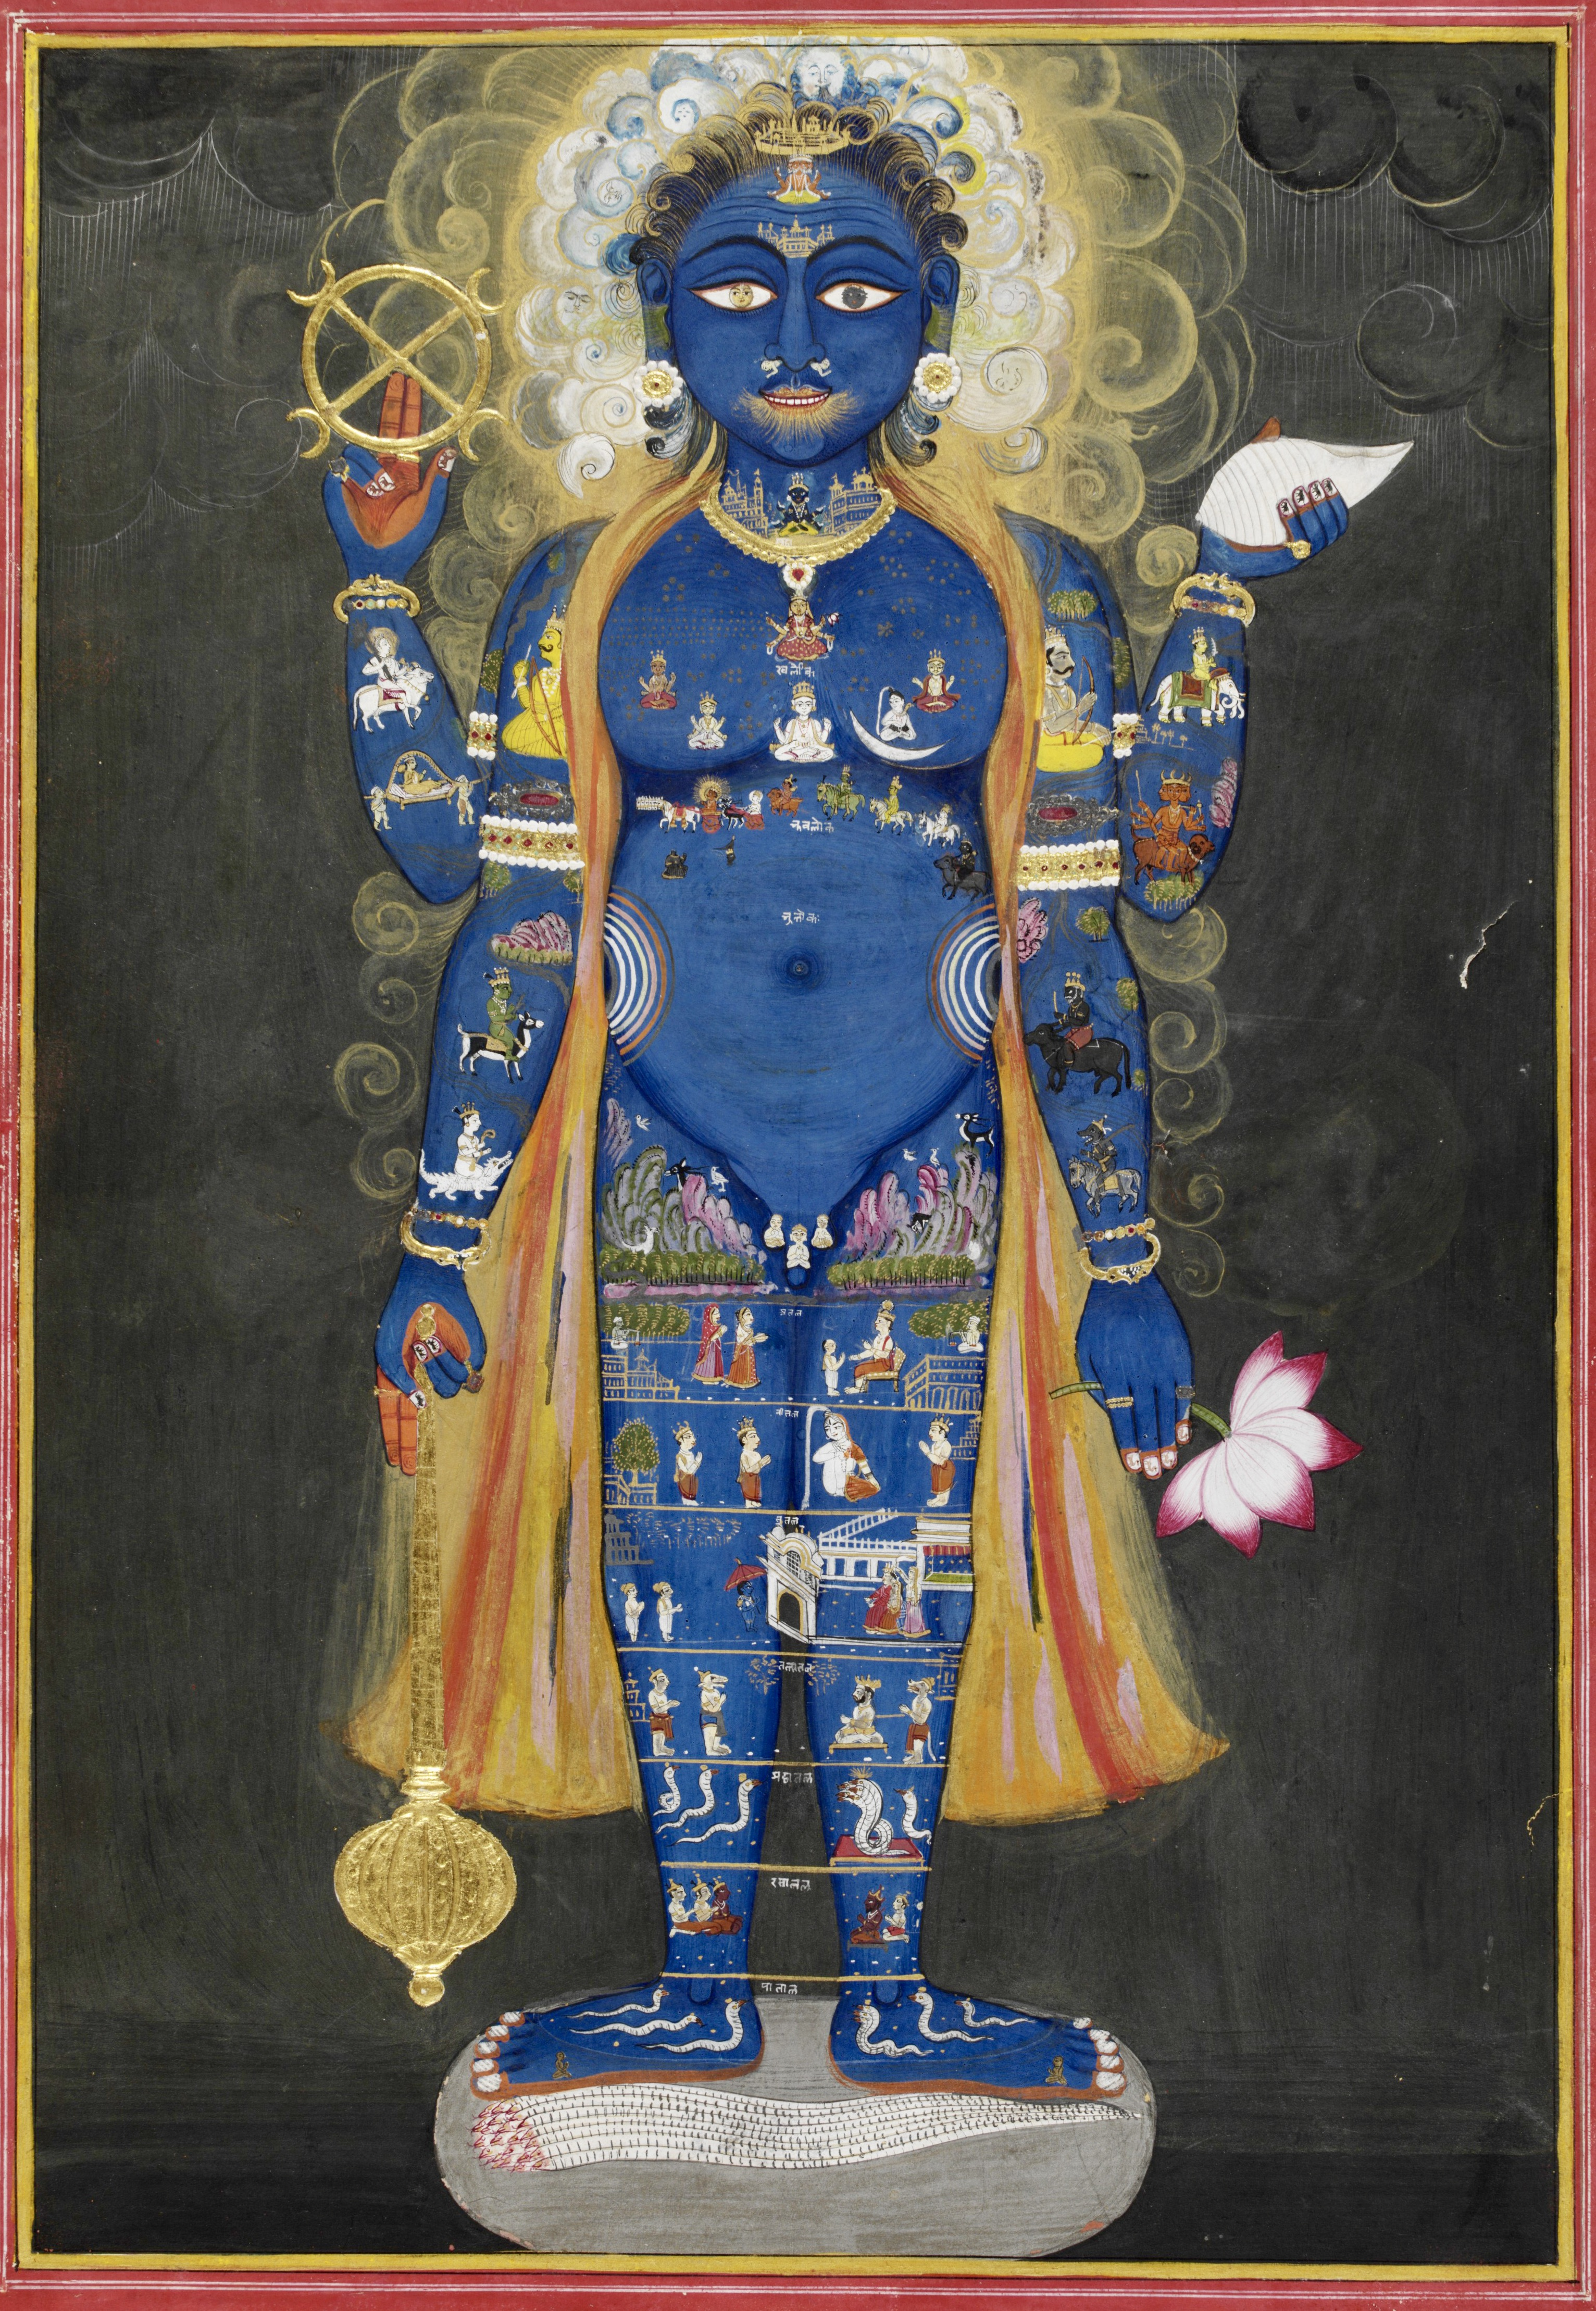
\includegraphics[width=1\textwidth]{pics/Vishnu_Vishvarupa_cropped.jpg}
	\caption{Viṣṇu Viśvarūpa, India, Rajasthan, Jaipur, ca. 1800–1820, Opaque watercolor and gold on paper, 38.5 × 28 cm, Victoria and Albert Museum, London, Given by Mrs. Gerald Clark.}
	\label{fig1}
      \end{figure}
\clearpage
  \begin{figure}[ht]
	\centering
  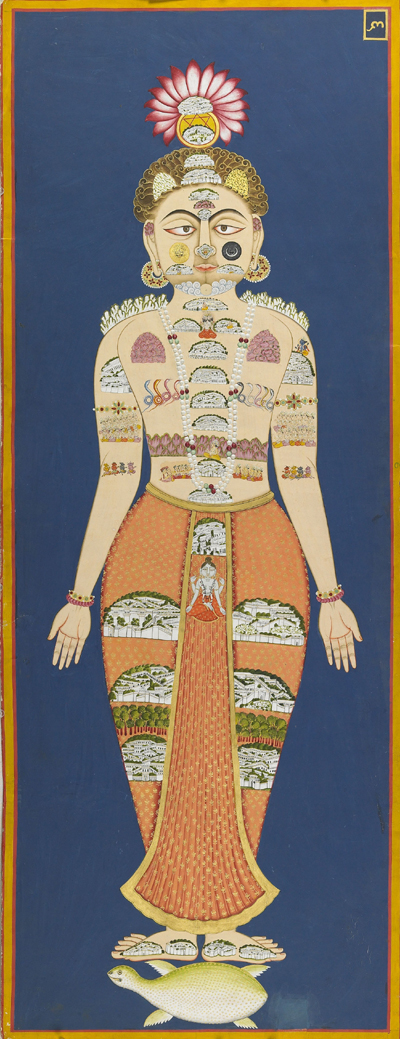
\includegraphics[width=0.5\textwidth]{pics/The_Equivalence_of_Self_and_Universe_(detail),_folio_6_from_the_Siddha_Siddhanta_Paddhati,_(Bulaki),_1824_(Samvat_1881);_122_x_46_cm._Mehrangarh_Museum_Trust..jpg}
	\caption{The Equivalence of Self and Universe (detail), folio 6 from the \textit{Siddhasiddhāntapaddhati} (Bulaki), India, Rajasthan, Jodhpur, 1824 (Samvat 1881), 122 x 46 cm, RJS 2378, Mehragarh Museum Trust.}
	\label{fig2}
      \end{figure}
      % \end{landscape}


\chapter{Bibliography}
 \label{sec:bibli}
   \clearpage
\newpage 
\thispagestyle{empty}
\quad  \addtocounter{page}{-1}

\printbibliography[heading=subbibintoc, title=Consulted Manuscripts, keyword=codex]

\printbibliography[heading=subbibintoc, title=Printed Editions, keyword=printsource]

\printbibliography[heading=subbibintoc, title=Secondary Literature, keyword=seclit]

\printbibliography[heading=subbibintoc, title=Online Sources, keyword=onlinesource]

\end{document}
